% This file was converted to LaTeX by Writer2LaTeX ver. 1.6.1
% see http://writer2latex.sourceforge.net for more info
\documentclass[a4paper,dvipdfmx]{jarticle}
\usepackage[latin1]{inputenc}
\usepackage{amsmath}
\usepackage{amssymb,amsfonts,textcomp}
\usepackage[T1]{fontenc}
\usepackage[english]{babel}
\usepackage{color}
\usepackage{array}
\usepackage{supertabular}
\usepackage{hhline}
\usepackage{hyperref}
\hypersetup{dvipdfmx, colorlinks=true, linkcolor=blue, citecolor=blue, filecolor=blue, urlcolor=blue, pdftitle=子どもIT未来塾 第5回, pdfauthor=, pdfsubject=, pdfkeywords=}
\usepackage[dvipdfmx]{graphicx}
\providecommand\textsubscript[1]{\ensuremath{{}_{\text{#1}}}}
\setcounter{secnumdepth}{3}
\renewcommand\thesection{\arabic{section}}
\renewcommand\thesubsection{\arabic{section}.\arabic{subsection}}
\renewcommand\thesubsubsection{\arabic{section}.\arabic{subsection}.\arabic{subsubsection}}
\makeatletter
\newcommand\arraybslash{\let\\\@arraycr}
\makeatother
% Page layout (geometry)
\setlength\voffset{-1in}
\setlength\hoffset{-1in}
\setlength\topmargin{2cm}
\setlength\oddsidemargin{2cm}
\setlength\textheight{24.770668cm}
\setlength\textwidth{17.006cm}
\setlength\footskip{26.144882pt}
\setlength\headheight{0cm}
\setlength\headsep{0cm}
% Footnote rule
\setlength{\skip\footins}{0.12cm}
\renewcommand\footnoterule{\vspace*{-0.018cm}\setlength\leftskip{0pt}\setlength\rightskip{0pt plus 1fil}\noindent\textcolor{black}{\rule{0.25\columnwidth}{0.018cm}}\vspace*{0.102cm}}
% Pages styles
\makeatletter
\newcommand\ps@Standard{
  \renewcommand\@oddhead{}
  \renewcommand\@evenhead{}
  \renewcommand\@oddfoot{2021年\hfill 子どもIT未来塾 第5回\hfill Page \thepage{}\ of ?}
  \renewcommand\@evenfoot{\@oddfoot}
  \renewcommand\thepage{\arabic{page}}
}
\newcommand\ps@FirstPage{
  \renewcommand\@oddhead{}
  \renewcommand\@evenhead{}
  \renewcommand\@oddfoot{}
  \renewcommand\@evenfoot{\@oddfoot}
  \renewcommand\thepage{\arabic{page}}
}
\makeatother
\pagestyle{Standard}
\setlength\tabcolsep{1mm}
\renewcommand\arraystretch{1.3}
% Non-floating captions
\makeatletter
\newcommand\captionof[1]{\def\@captype{#1}\caption}
\makeatother
\newcounter{qwertyc}
\renewcommand\theqwertyc{\arabic{qwertyc}}
\newcounter{qwertya}
\renewcommand\theqwertya{\arabic{qwertya}}
\newcounter{qwertyb}
\renewcommand\theqwertyb{\arabic{qwertyb}}
\newcounter{List}
\renewcommand\theList{\arabic{List}}
\newcounter{qwerty}
\renewcommand\theqwerty{\arabic{qwerty}}
\title{子どもIT未来塾 第5回}
\author{}
\date{2021-09-18}
\begin{document}
\clearpage\setcounter{page}{1}\pagestyle{Standard}
\thispagestyle{FirstPage}

\bigskip

\clearpage\section[\ センサーの基本]{%\rmfamily
\ センサーの基本}
%\begin{figure}

\begin{minipage}{17.369cm}
\clearpage\setcounter{page}{1}\pagestyle{Standard}
\thispagestyle{FirstPage}
{\centering\bfseries
子どもIT未来塾 第5回
\par}

{\centering\bfseries
Raspberry Piをリモコンにしてみよう
\par}

{\centering\bfseries
2021年
\par}


\bigskip

{\centering\bfseries
奥山祐市
\par}

{\centering\bfseries
小堺美咲
\par}

{\centering\bfseries
荒川麻衣子
\par}

{\centering\bfseries
新明洋平
\par}
\end{minipage}
%\end{figure}
\subsection[センサーってなんだろう?]{\rmfamily
センサーってなんだろう?}
{\mdseries
センサーは身の回りの世界の情報を調べ、コンピュータに伝えるためのものです。明るさや温度、湿度などを調べることができるセンサーボードは第3回の授業で扱いました。しかし、センサーにはまだまだたくさんの種類があり、出来ることがもっとたくさんあります。まず、車で使われているセンサーを見てみましょう。}



%\begin{figure}
\centering
\begin{minipage}{16.799cm}

\begin{minipage}{12.155cm}
{\upshape
 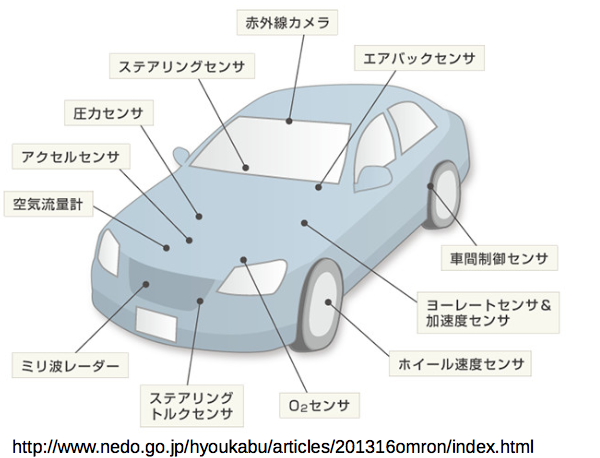
\includegraphics[width=12.155cm,height=8.851cm]{text05-img/text05-img001.png} %\newline
図 \stepcounter{qwerty}{\theqwerty}:
自動車に使われているセンサー(https://www.nedo.go.jp/hyoukabu/articles/201316omron/index.html)}
\end{minipage}\end{minipage}
%\end{figure}
\begin{flushleft}
\tablefirsthead{}
\tablehead{}
\tabletail{}
\tablelasttail{}
\begin{supertabular}{|m{7.42cm}|m{9.193cm}|}
\hline
\centering センサーの種類 &
\centering\arraybslash できること\\\hline
赤外線カメラ &
暗闇で物を見ることができる\\\hline
ステアリングセンサ &
ハンドルの回しぐあいによってタイヤの方向を決める\\\hline
圧力センサ &
圧力を調べる\\\hline
アクセルセンサ &
アクセルペダルの踏み具合を調べる\\\hline
ミリ波レーダー &
車の前に物があるかを調べる\\\hline
トルクセンサ &
ねじれの強さを調べる\\\hline
O\textsubscript{2}センサ &
燃料の働き具合を空気の酸素(O\textsubscript{2})量で調べる\\\hline
ホイール速度センサ &
タイヤの回転速度を調べる\\\hline
ヨーレートセンサ&加速度センサ &
車の速さを調べる\\\hline
車間制御センサ &
前の車との距離を調べる\\\hline
エアバックセンサ &
車の衝突を感知して瞬時にエアバッグを膨らませる\\\hline
\end{supertabular}
\end{flushleft}

\bigskip

このように、機械ではたくさんのセンサーが使われています。今日の授業では新しいセンサーをいくつか扱います。どのセンサーが何に使えそうか、何に使われていそうかを考えながら使ってみましょう。


\bigskip

{\bfseries
問題 5-\stepcounter{qwertya}{\theqwertya}}

センサーとはなんだろう。説明してみよう。

\begin{enumerate}
\item[] 
\bigskip

答え.                             
\end{enumerate}

\bigskip

{\bfseries
問題 5-\stepcounter{qwertya}{\theqwertya}}

車で使われているセンサーを3つ書いてみよう。

%\setcounter{saveenum}{\value{enumi}}
\begin{enumerate}
%\setcounter{enumi}{\value{saveenum}}
\item[] 
\bigskip
\end{enumerate}
\ \ 答え.                             


\bigskip

\subsection[]{\rmfamily }
\clearpage\subsection[アナログ信号とデジタル信号]{\rmfamily
アナログ信号とデジタル信号}
センサーには二種類あり、デジタル信号とアナログ信号と呼ばれる信号のどちらを使うかで分けられています。二つの信号には以下の図のような違いがあります。


\bigskip



%\begin{figure}
\centering
\begin{minipage}{9.243cm}

\begin{minipage}{8.601cm}
{\upshape
 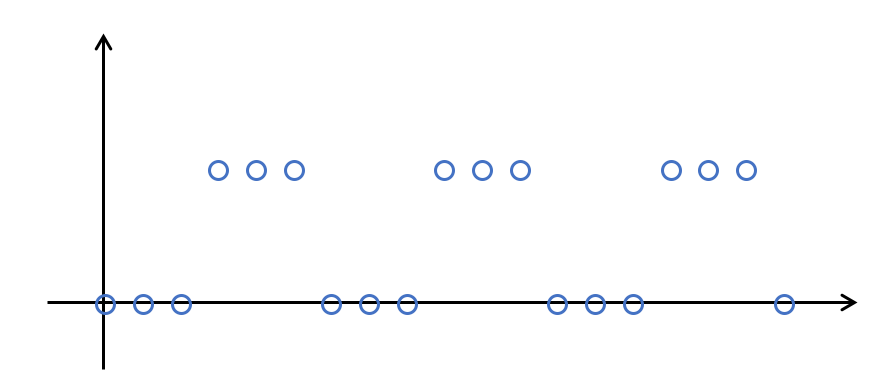
\includegraphics[width=8.601cm,height=3.701cm]{text05-img/text05-img002.png} \newline
図 {\refstepcounter{qwerty}\theqwerty\label{seq:ref1}}: デジタル信号の例}
\end{minipage}\begin{minipage}{2.31cm}
値
\end{minipage}\begin{minipage}{1.888cm}
値
\end{minipage}\end{minipage}
%\end{figure}
%\begin{figure}
\centering
\begin{minipage}{9.447cm}

\begin{minipage}{8.8cm}
{\upshape
 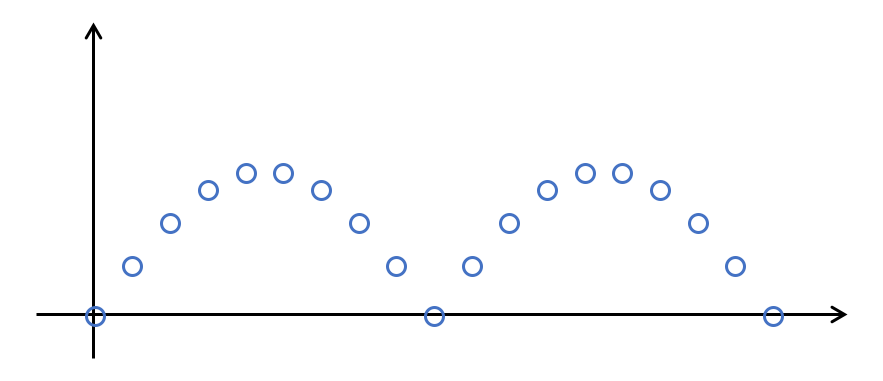
\includegraphics[width=8.8cm,height=3.791cm]{text05-img/text05-img003.png} \newline
図 {\refstepcounter{qwerty}\theqwerty\label{seq:ref2}}: アナログ信号の例}
\end{minipage}\begin{minipage}{2.31cm}
値
\end{minipage}\begin{minipage}{1.999cm}
時間


\bigskip
\end{minipage}\begin{minipage}{2.31cm}
時間


\bigskip
\end{minipage}\end{minipage}
%\end{figure}

\bigskip


\bigskip


\bigskip


\bigskip


\bigskip


\bigskip


\bigskip

?~\ref{seq:ref1}と?~\ref{seq:ref2}はコンピュータで使われている信号をグラフにしたものです。まず、二つのグラフを見比べてみましょう。授業で使用するセンサーのデジタル信号は、?~\ref{seq:ref1}のように0か1のみを表すことができます。一方授業で使用するアナログ信号は、?~\ref{seq:ref2}のように0〜1023の数字を表すことができます。デジタル信号はボタンが押されたか押されていないか、明かりがついたか消えたかなどのふた通りのものを表すときに使われ、アナログ信号は主に明るさや距離などの数を表すときに使われます。


\bigskip

\textbf{問題 5{}-\stepcounter{qwertya}{\theqwertya}}

{\mdseries
アナログ信号、デジタル信号の違いを書いてみましょう。}

\begin{enumerate}
\item[] 
\bigskip

答え.                             
\end{enumerate}
\clearpage\section[FaBoのブリックについて]{\rmfamily
FaBoのブリックについて}
\subsection[FaBoの使い方]{\rmfamily FaBoの使い方}
今日の授業ではFaBoのシールドとFaBoのブリックを使います。この二つは簡単にセンサーとRaspberry
Piとつなげるようにあらかじめ配線がされているものです。

\begin{center}
\tablefirsthead{}
\tablehead{}
\tabletail{}
\tablelasttail{}
\begin{supertabular}{|l|l|}
\hline
\multicolumn{1}{|c|}{\begin{minipage}{8.202cm}
\upshape \begin{minipage}{8.202cm}
\upshape  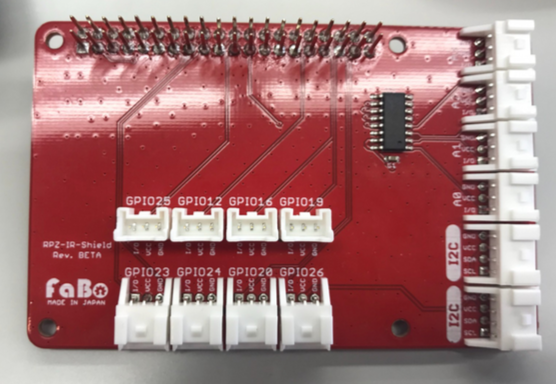
\includegraphics[width=8.202cm,height=5.867cm]{text05-img/text05-img004.png} \newline
図 \stepcounter{qwerty}{\theqwerty}: Faboのシールド\end{minipage}\end{minipage}} &
\multicolumn{1}{c|}{\centering
\begin{minipage}{5.819cm}
\upshape  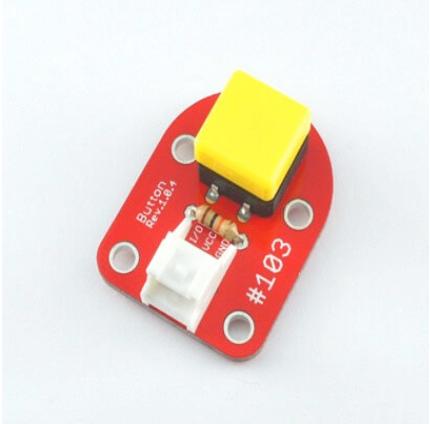
\includegraphics[width=5.819cm,height=5.738cm]{text05-img/text05-img005.png} \newline
図 \stepcounter{qwerty}{\theqwerty}: Faboのブリック\end{minipage}
}\\\hline
\end{supertabular}
\end{center}

\bigskip

豆電球が電池で動くように、ブリックはRaspberry
Piが電源となって動きます。本当ならばブリックとRaspberry
Piをプラスマイナス、ブリックの出力などを考えて繋がないといけません。しかし、FaBoのシールドとブリックは必要な配線がすでにされているため、自分でどう線を繋ぐかを考えなくても簡単に使えます。

それでは、さっそくFaBoをつかってみましょう。

{\color[rgb]{0.5019608,0.0,0.0}
注意!}

FaboのシールドをRaspberry
Piとつなげるときは、必ずRaspberry
Piをシャットダウンして電源を落としましょう。

\begin{enumerate}
\item \clearpage
Faboの電源を落とします。
\item FaBoのシールドをRaspberry
Piとつなげます。この時、なるべくシールドをまっすぐに押しこむようにしましょう。ピン(金属の棒の部分)を曲げないように注意してください。シールドにもトゲのある所があるのでケガをしないように注意しましょう。
\end{enumerate}


%\begin{figure}
\centering
\begin{minipage}{16.521cm}


\begin{minipage}{9.975cm}
{\upshape
 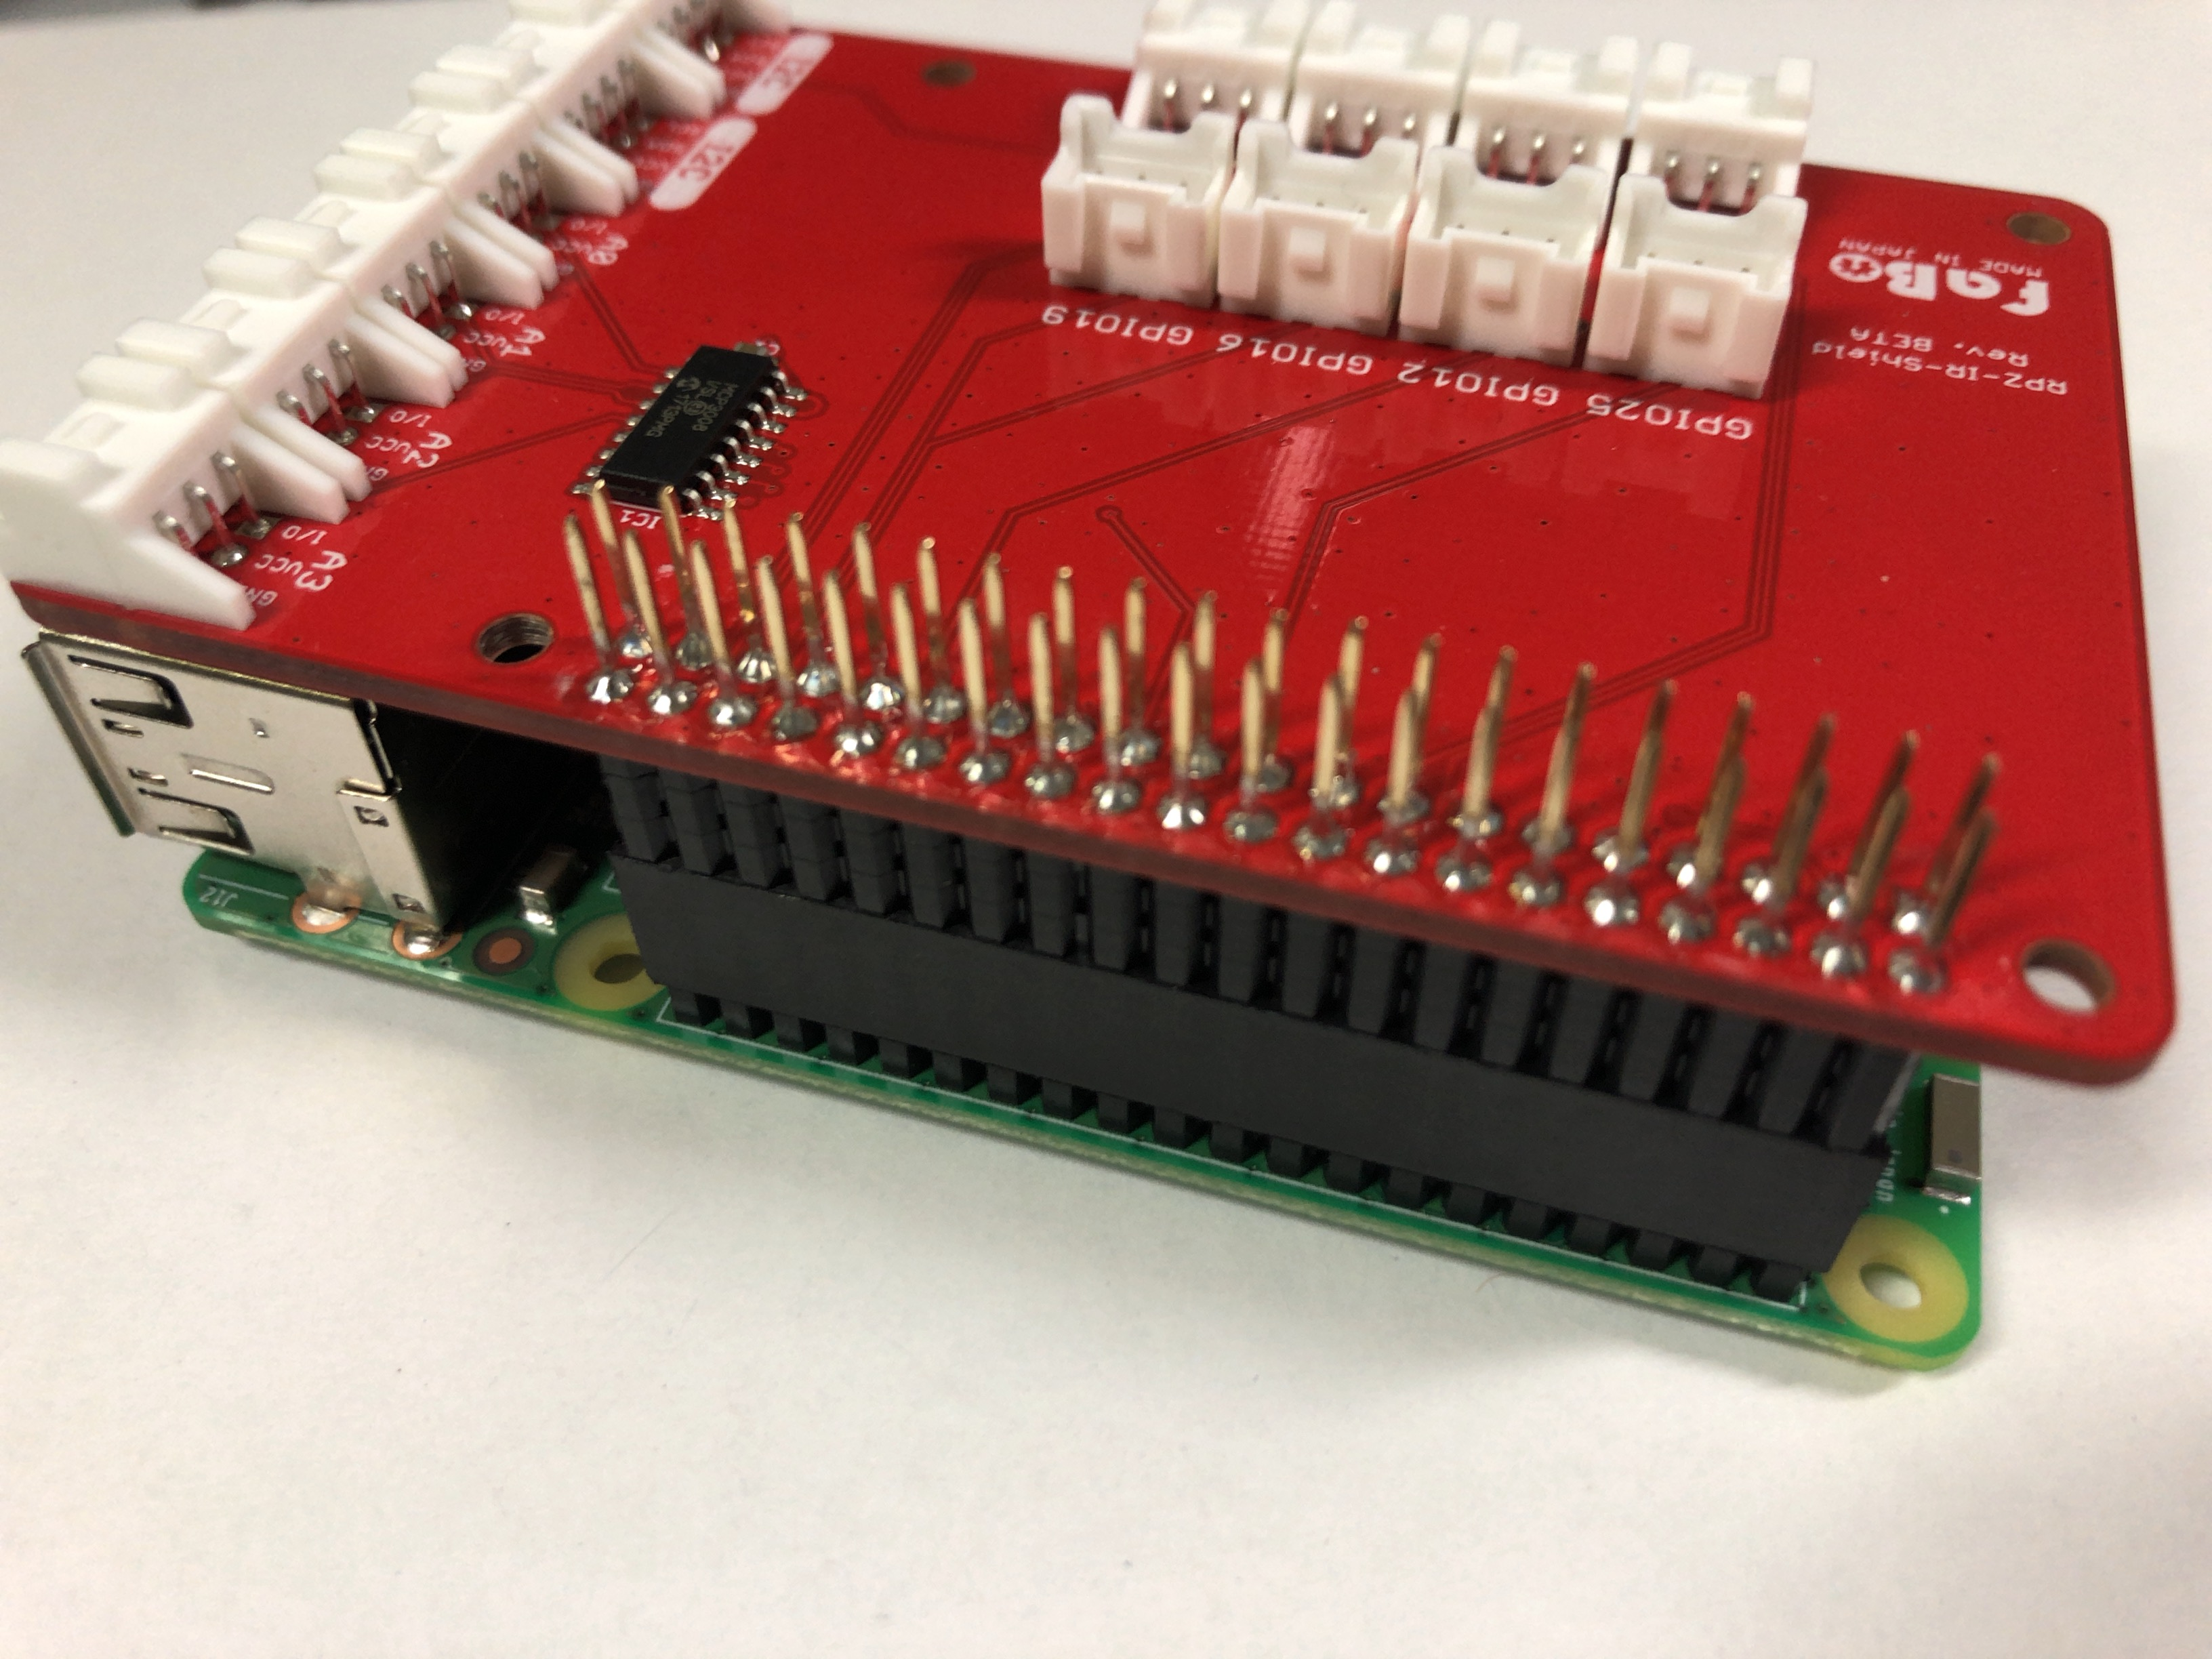
\includegraphics[width=8.966cm,height=5.969cm]{text05-img/text05-img006.jpg} \newline
図 \stepcounter{qwerty}{\theqwerty}: FaboのシールドとRaspberry
Piのせつぞく}
\end{minipage}
\bigskip
\end{minipage}
%\end{figure}
%\setcounter{saveenum}{\value{enumi}}
\begin{enumerate}
%\setcounter{enumi}{\value{saveenum}}
\item
LEDをケーブルとつなげましょう。奥までケーブルを押しこんでください。
\end{enumerate}


%\begin{figure}
\centering
\begin{minipage}{14.834cm}


\begin{minipage}{9.559cm}
{\upshape
 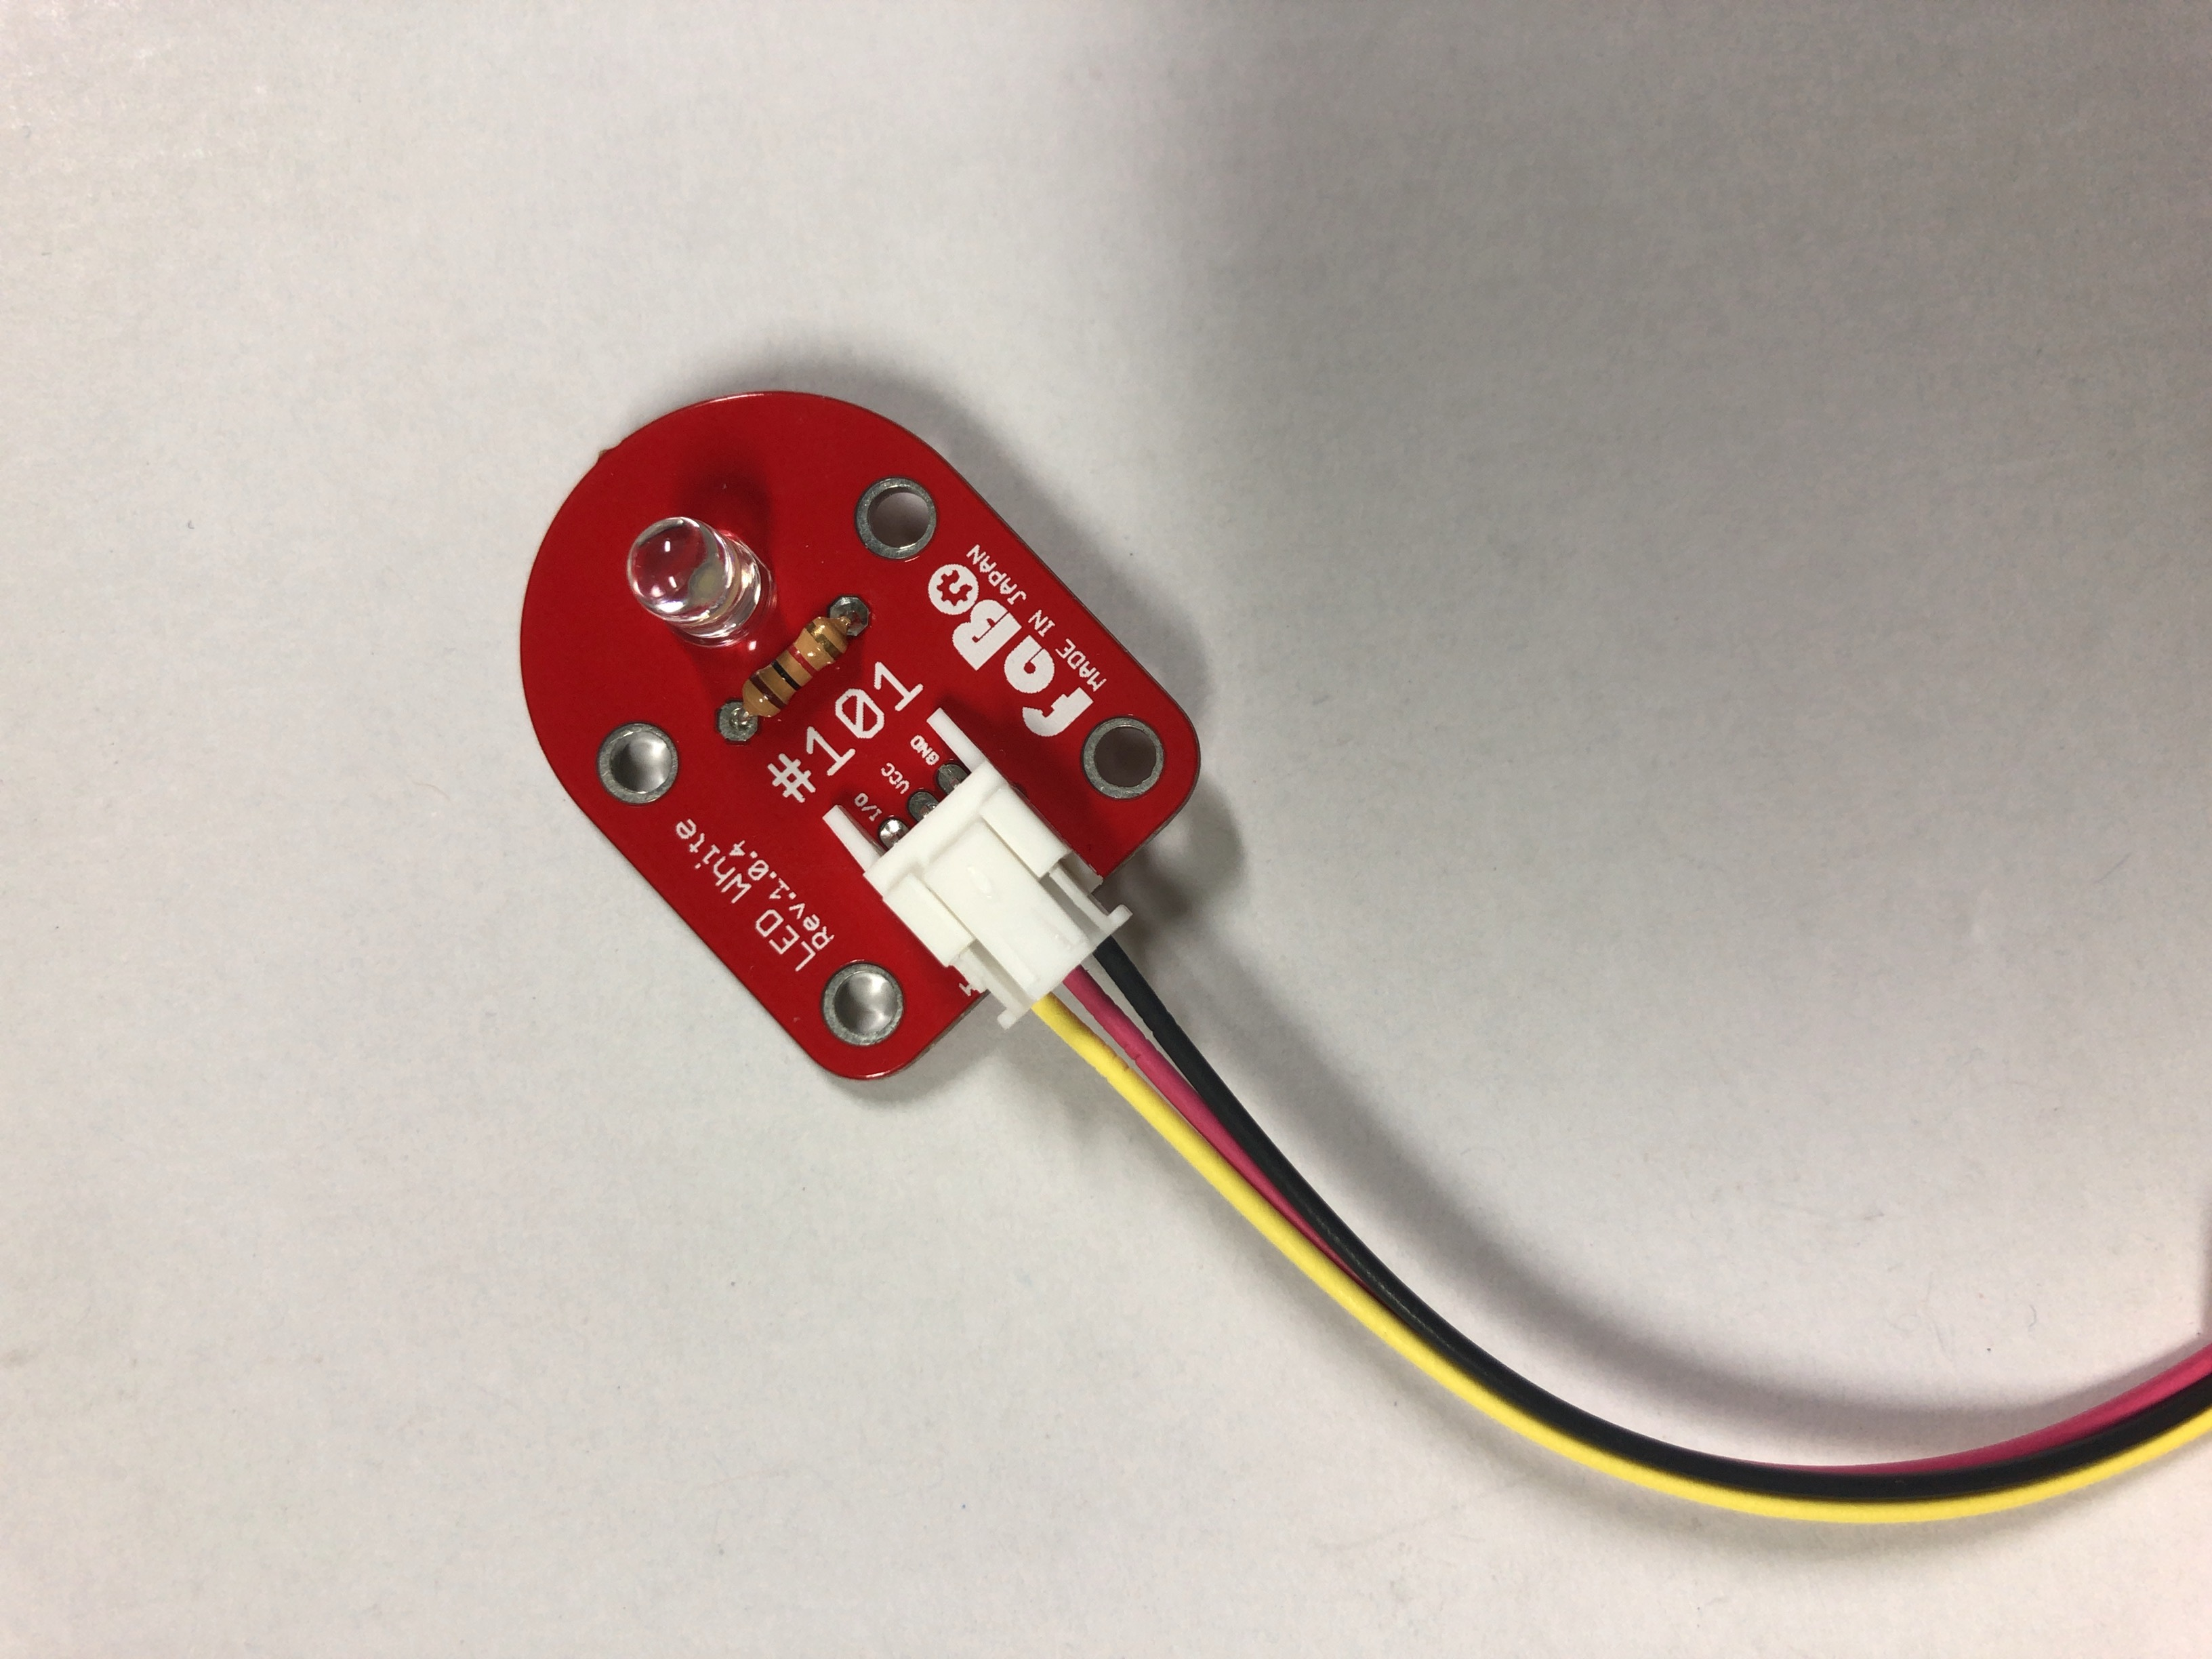
\includegraphics[width=9.559cm,height=5.787cm]{text05-img/text05-img007.jpg} \newline
図 \stepcounter{qwerty}{\theqwerty}:
Faboのブリックとケーブルのせつぞく}
\end{minipage}
\bigskip
\end{minipage}
%\end{figure}

\bigskip

%\setcounter{saveenum}{\value{enumi}}
\begin{enumerate}
%\setcounter{enumi}{\value{saveenum}}
\item \clearpage
シールドとケーブルをつなげましょう。今回はGPIO
23の所につなげます。このときも奥までケーブルを押しこんでください。\newline

%\begin{figure}
\centering
\begin{minipage}{15.669cm}


\begin{minipage}{9.237cm}
{\upshape
 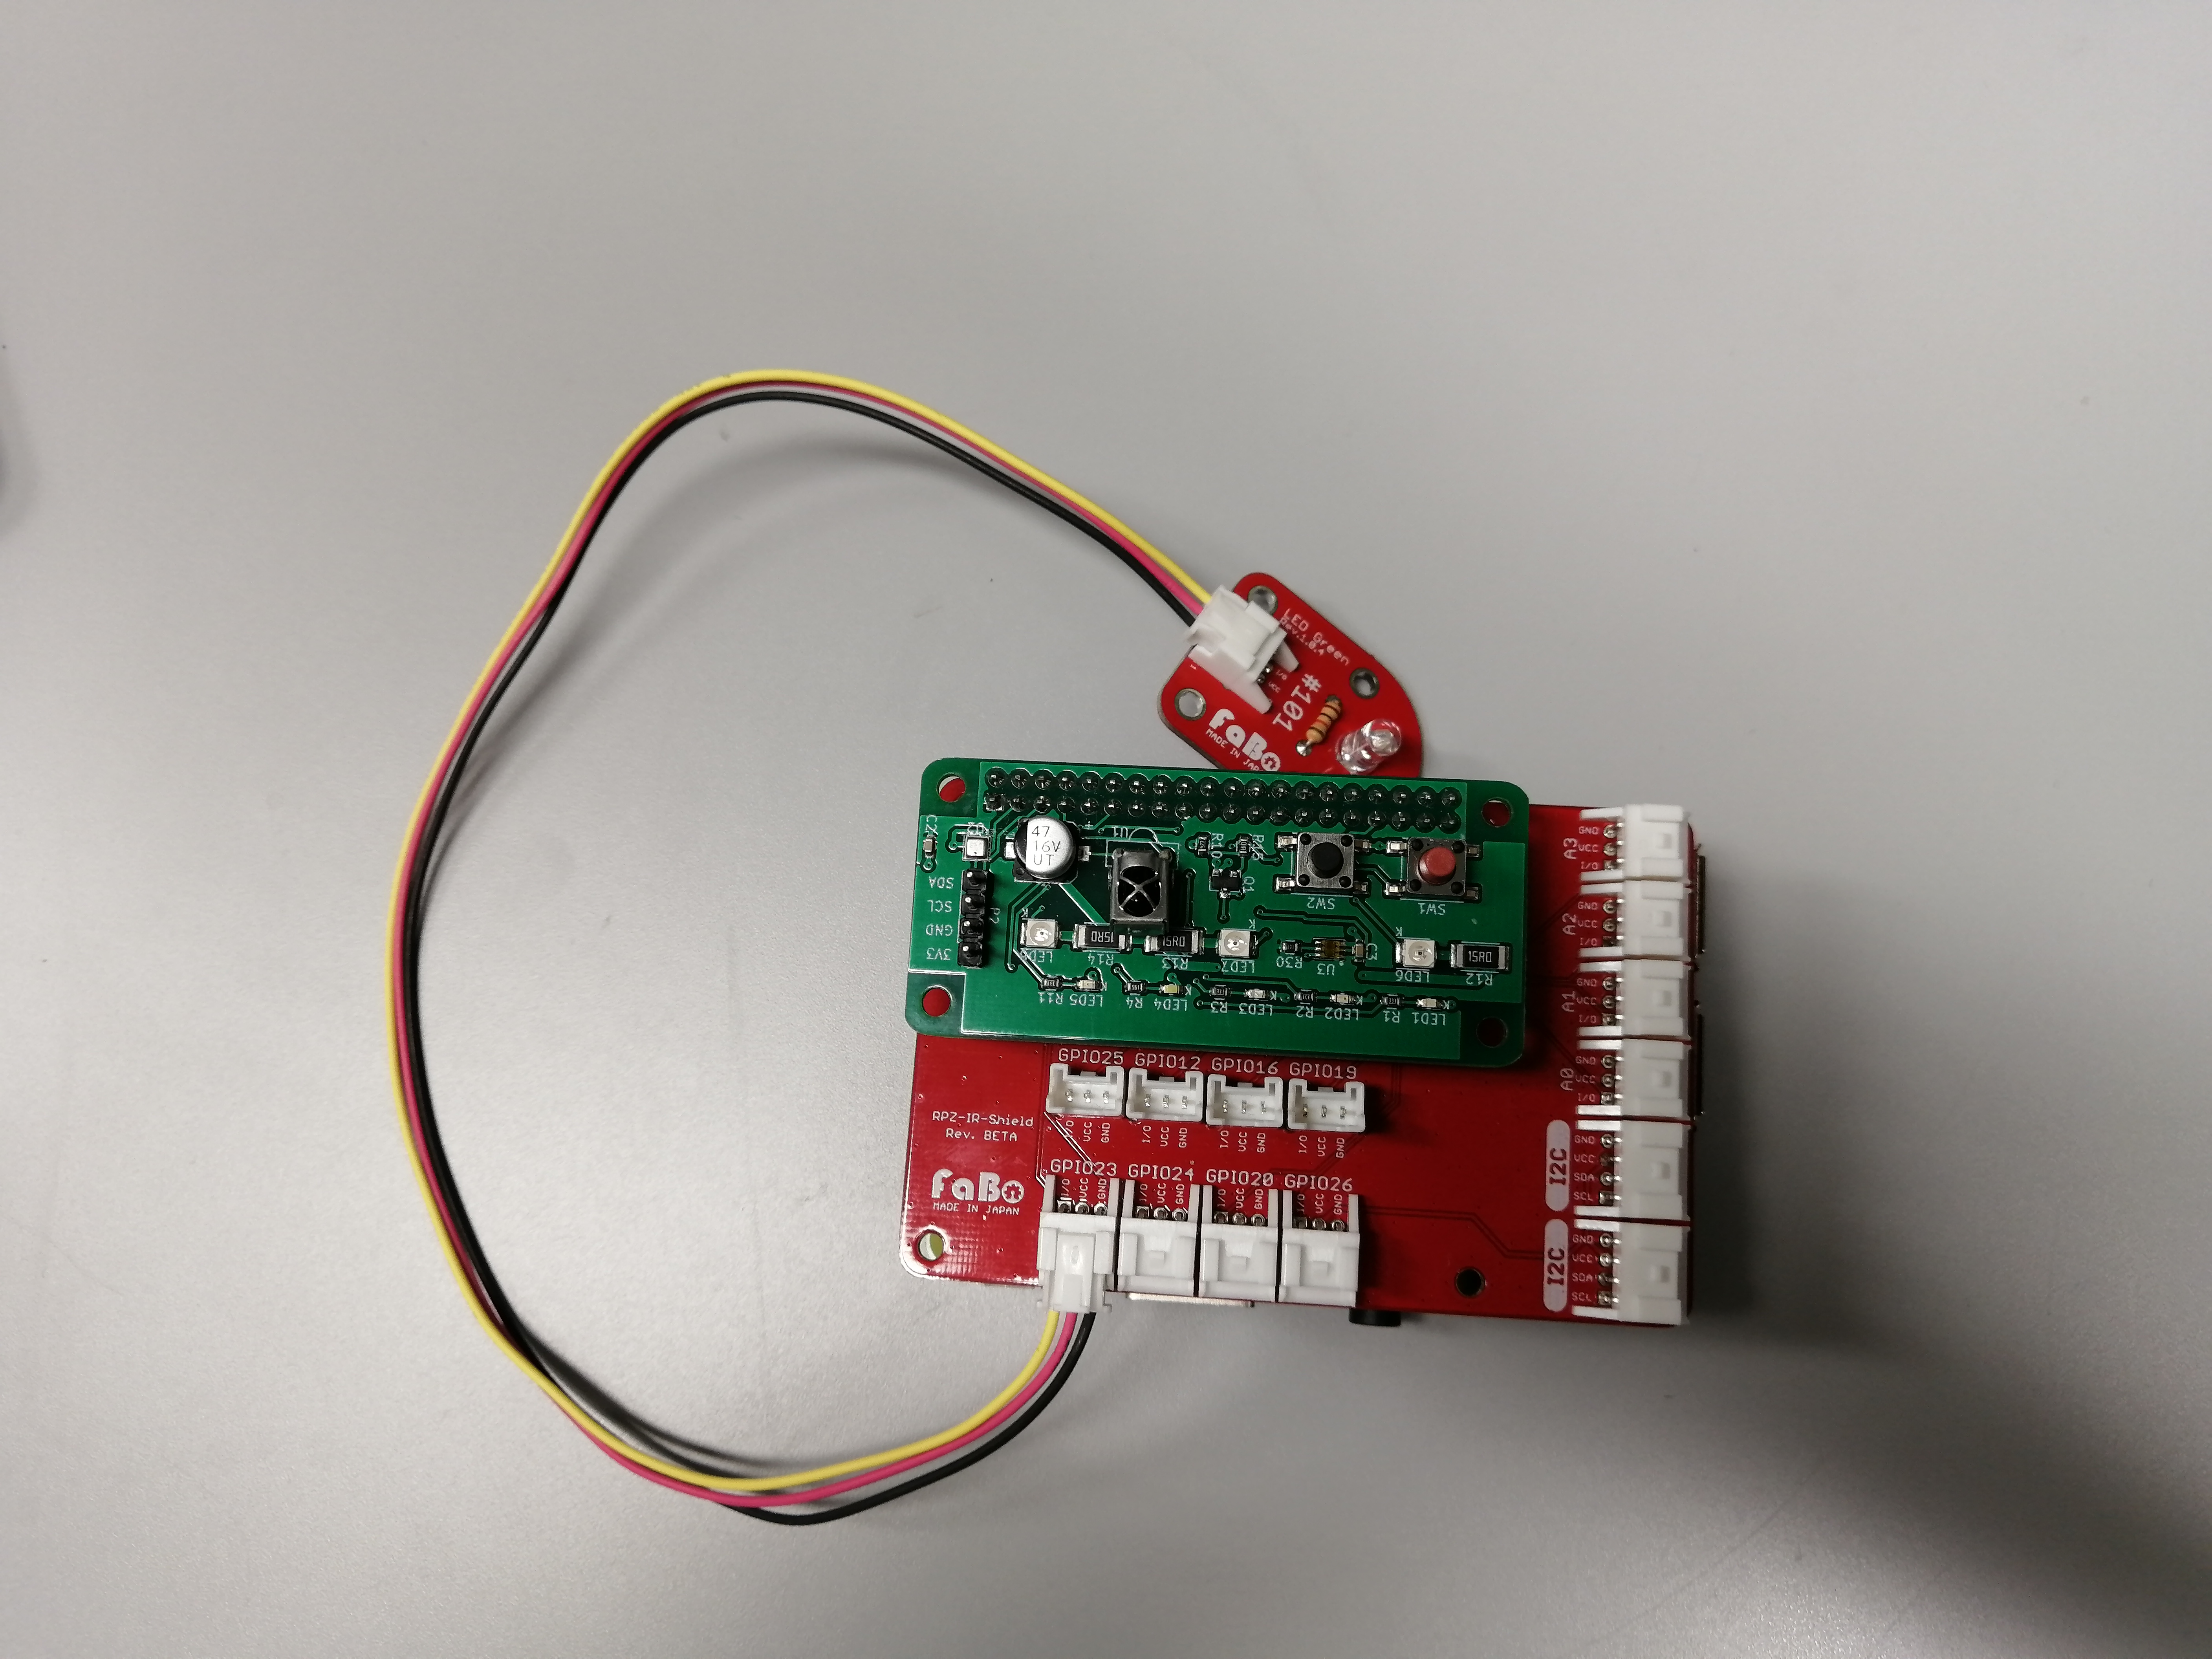
\includegraphics[width=9.237cm,height=5.408cm]{text05-img/text05-img008.jpg} \newline
図 \stepcounter{qwerty}{\theqwerty}:
Faboシールドとケーブルのせつぞく}
\end{minipage}
\bigskip
\end{minipage}
%\end{figure}
\item
ケーブルを外す時は、とがっているツメの部分を押して引きぬいてください。ぬけない時やわからない時は周りの先生に聞いてみましょう。
\end{enumerate}
\begin{center}
\tablefirsthead{}
\tablehead{}
\tabletail{}
\tablelasttail{}
\begin{supertabular}{m{8.302cm}m{8.304cm}}
\begin{minipage}{7.768cm}
{\upshape  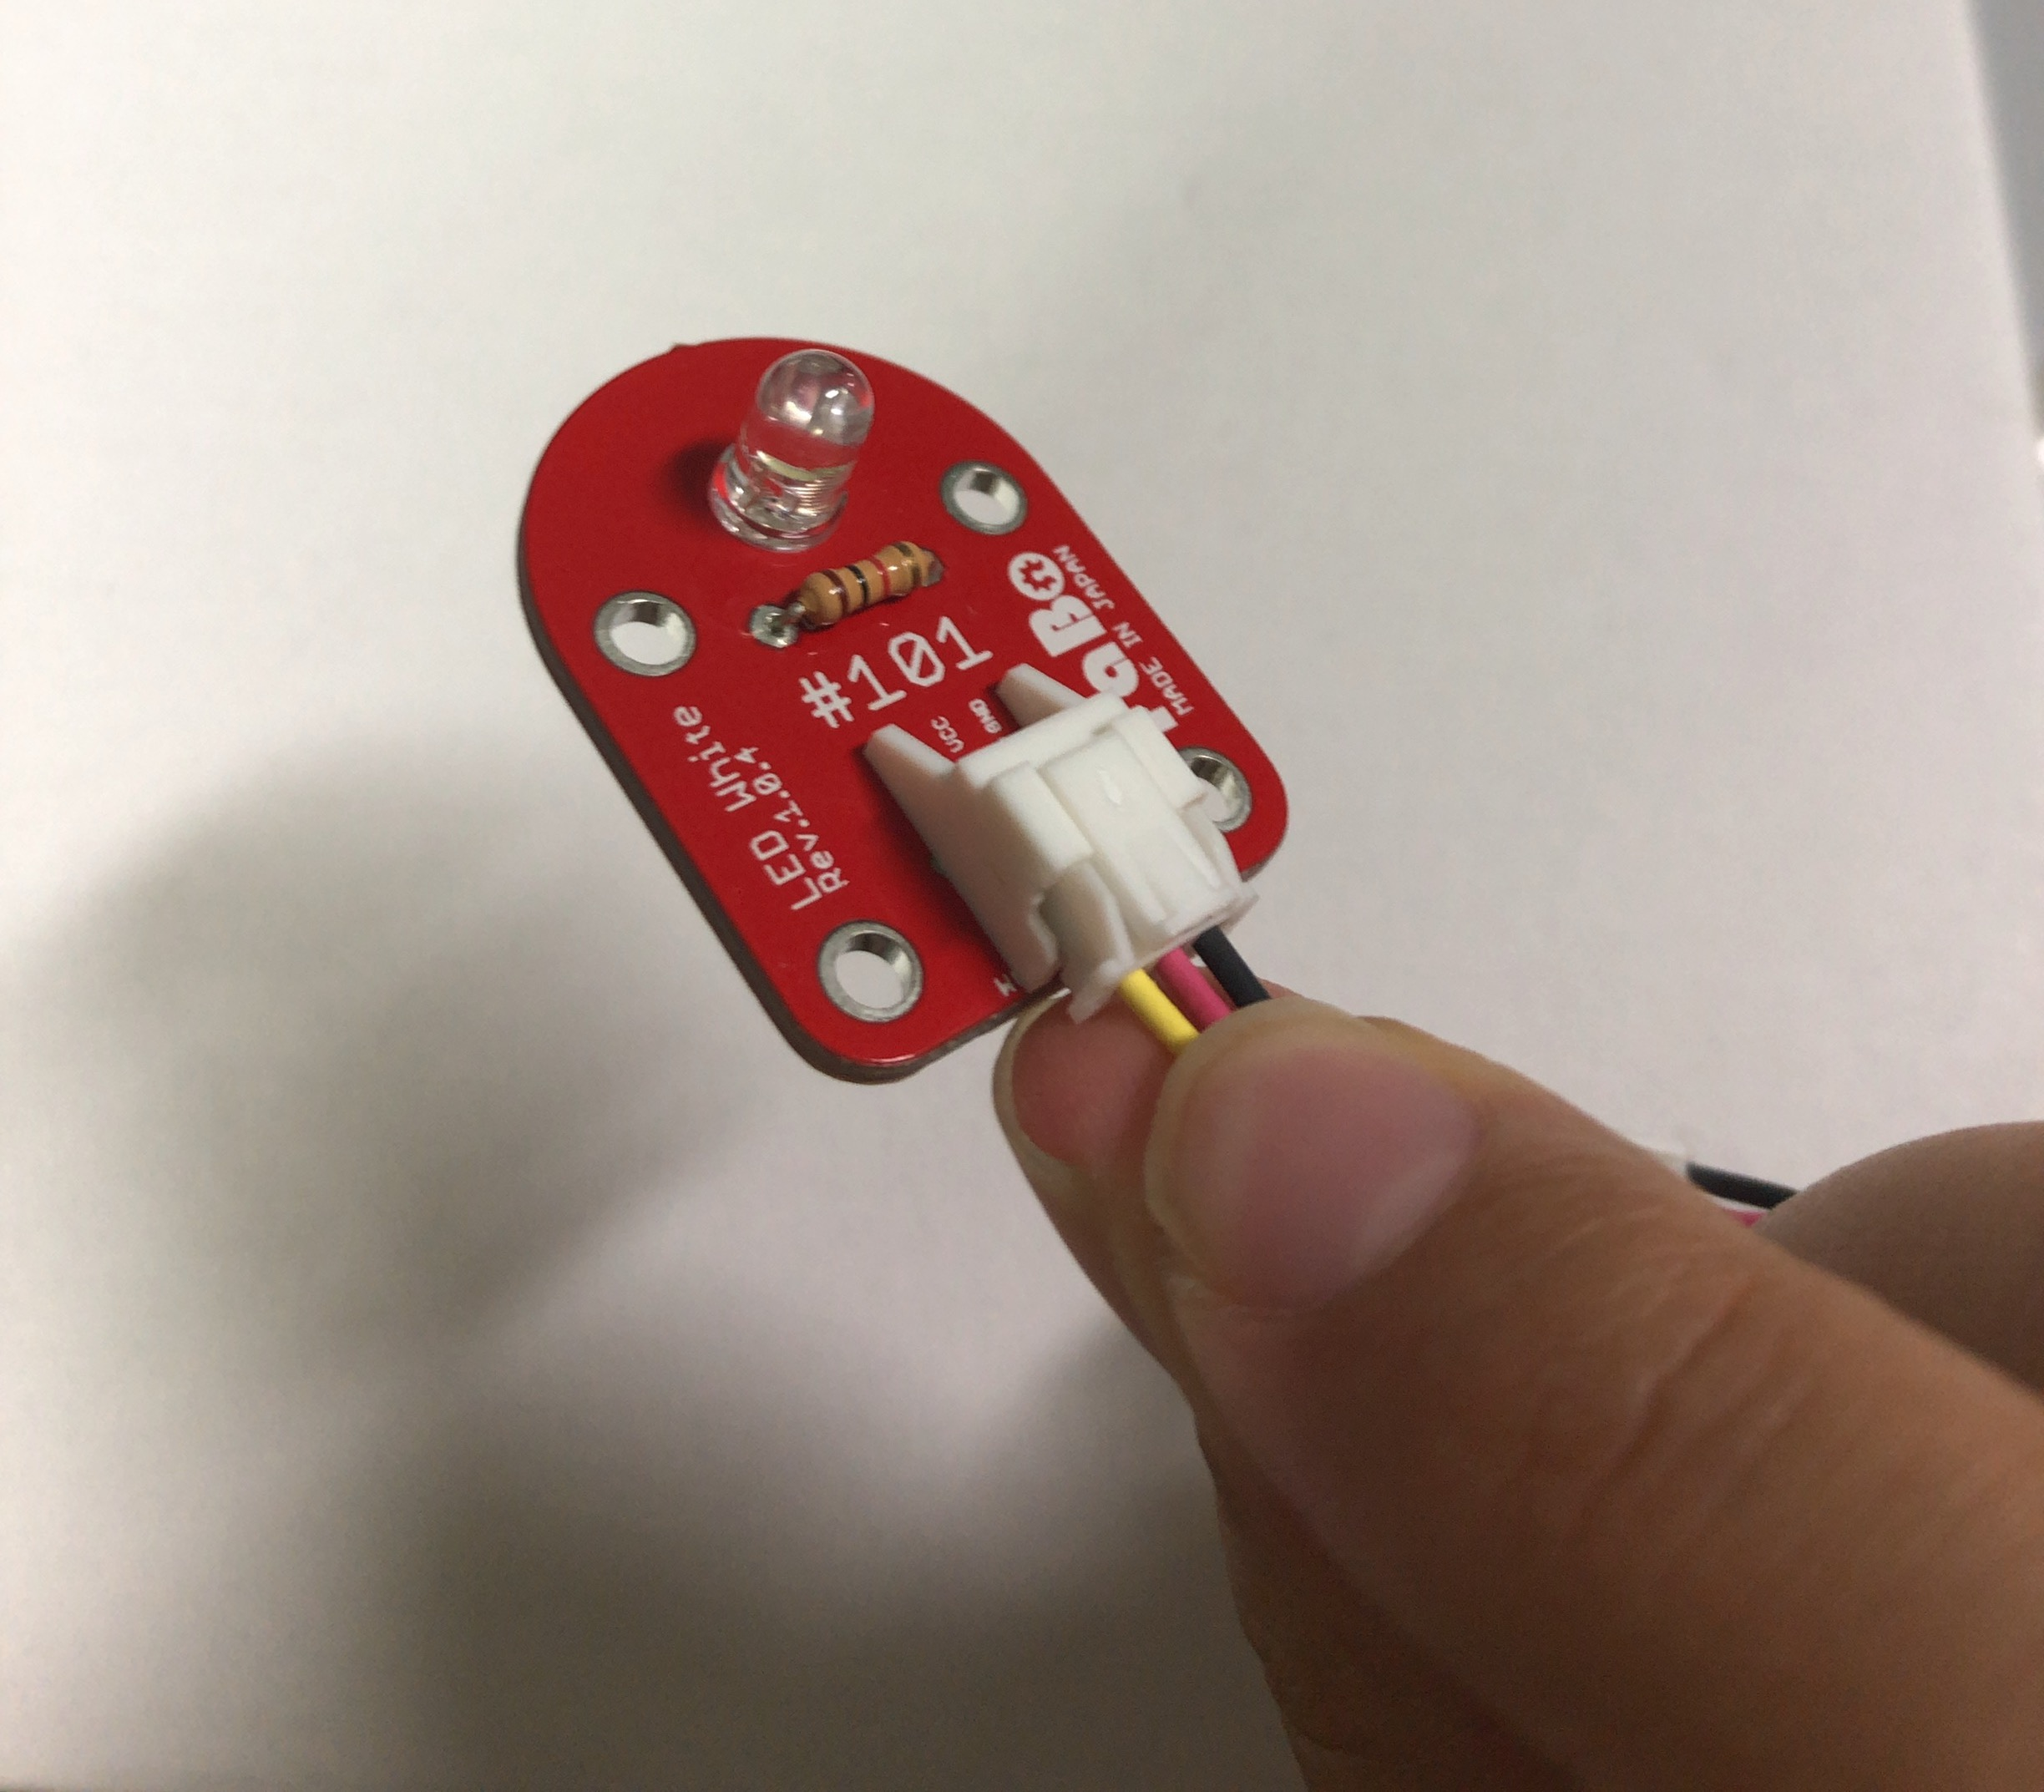
\includegraphics[width=7.768cm,height=5.68cm]{text05-img/text05-img009.jpg} \newline
図 \stepcounter{qwerty}{\theqwerty}: ケーブルのツメ}\end{minipage}
 &
\arraybslash 
\begin{minipage}{7.281cm}
{\upshape  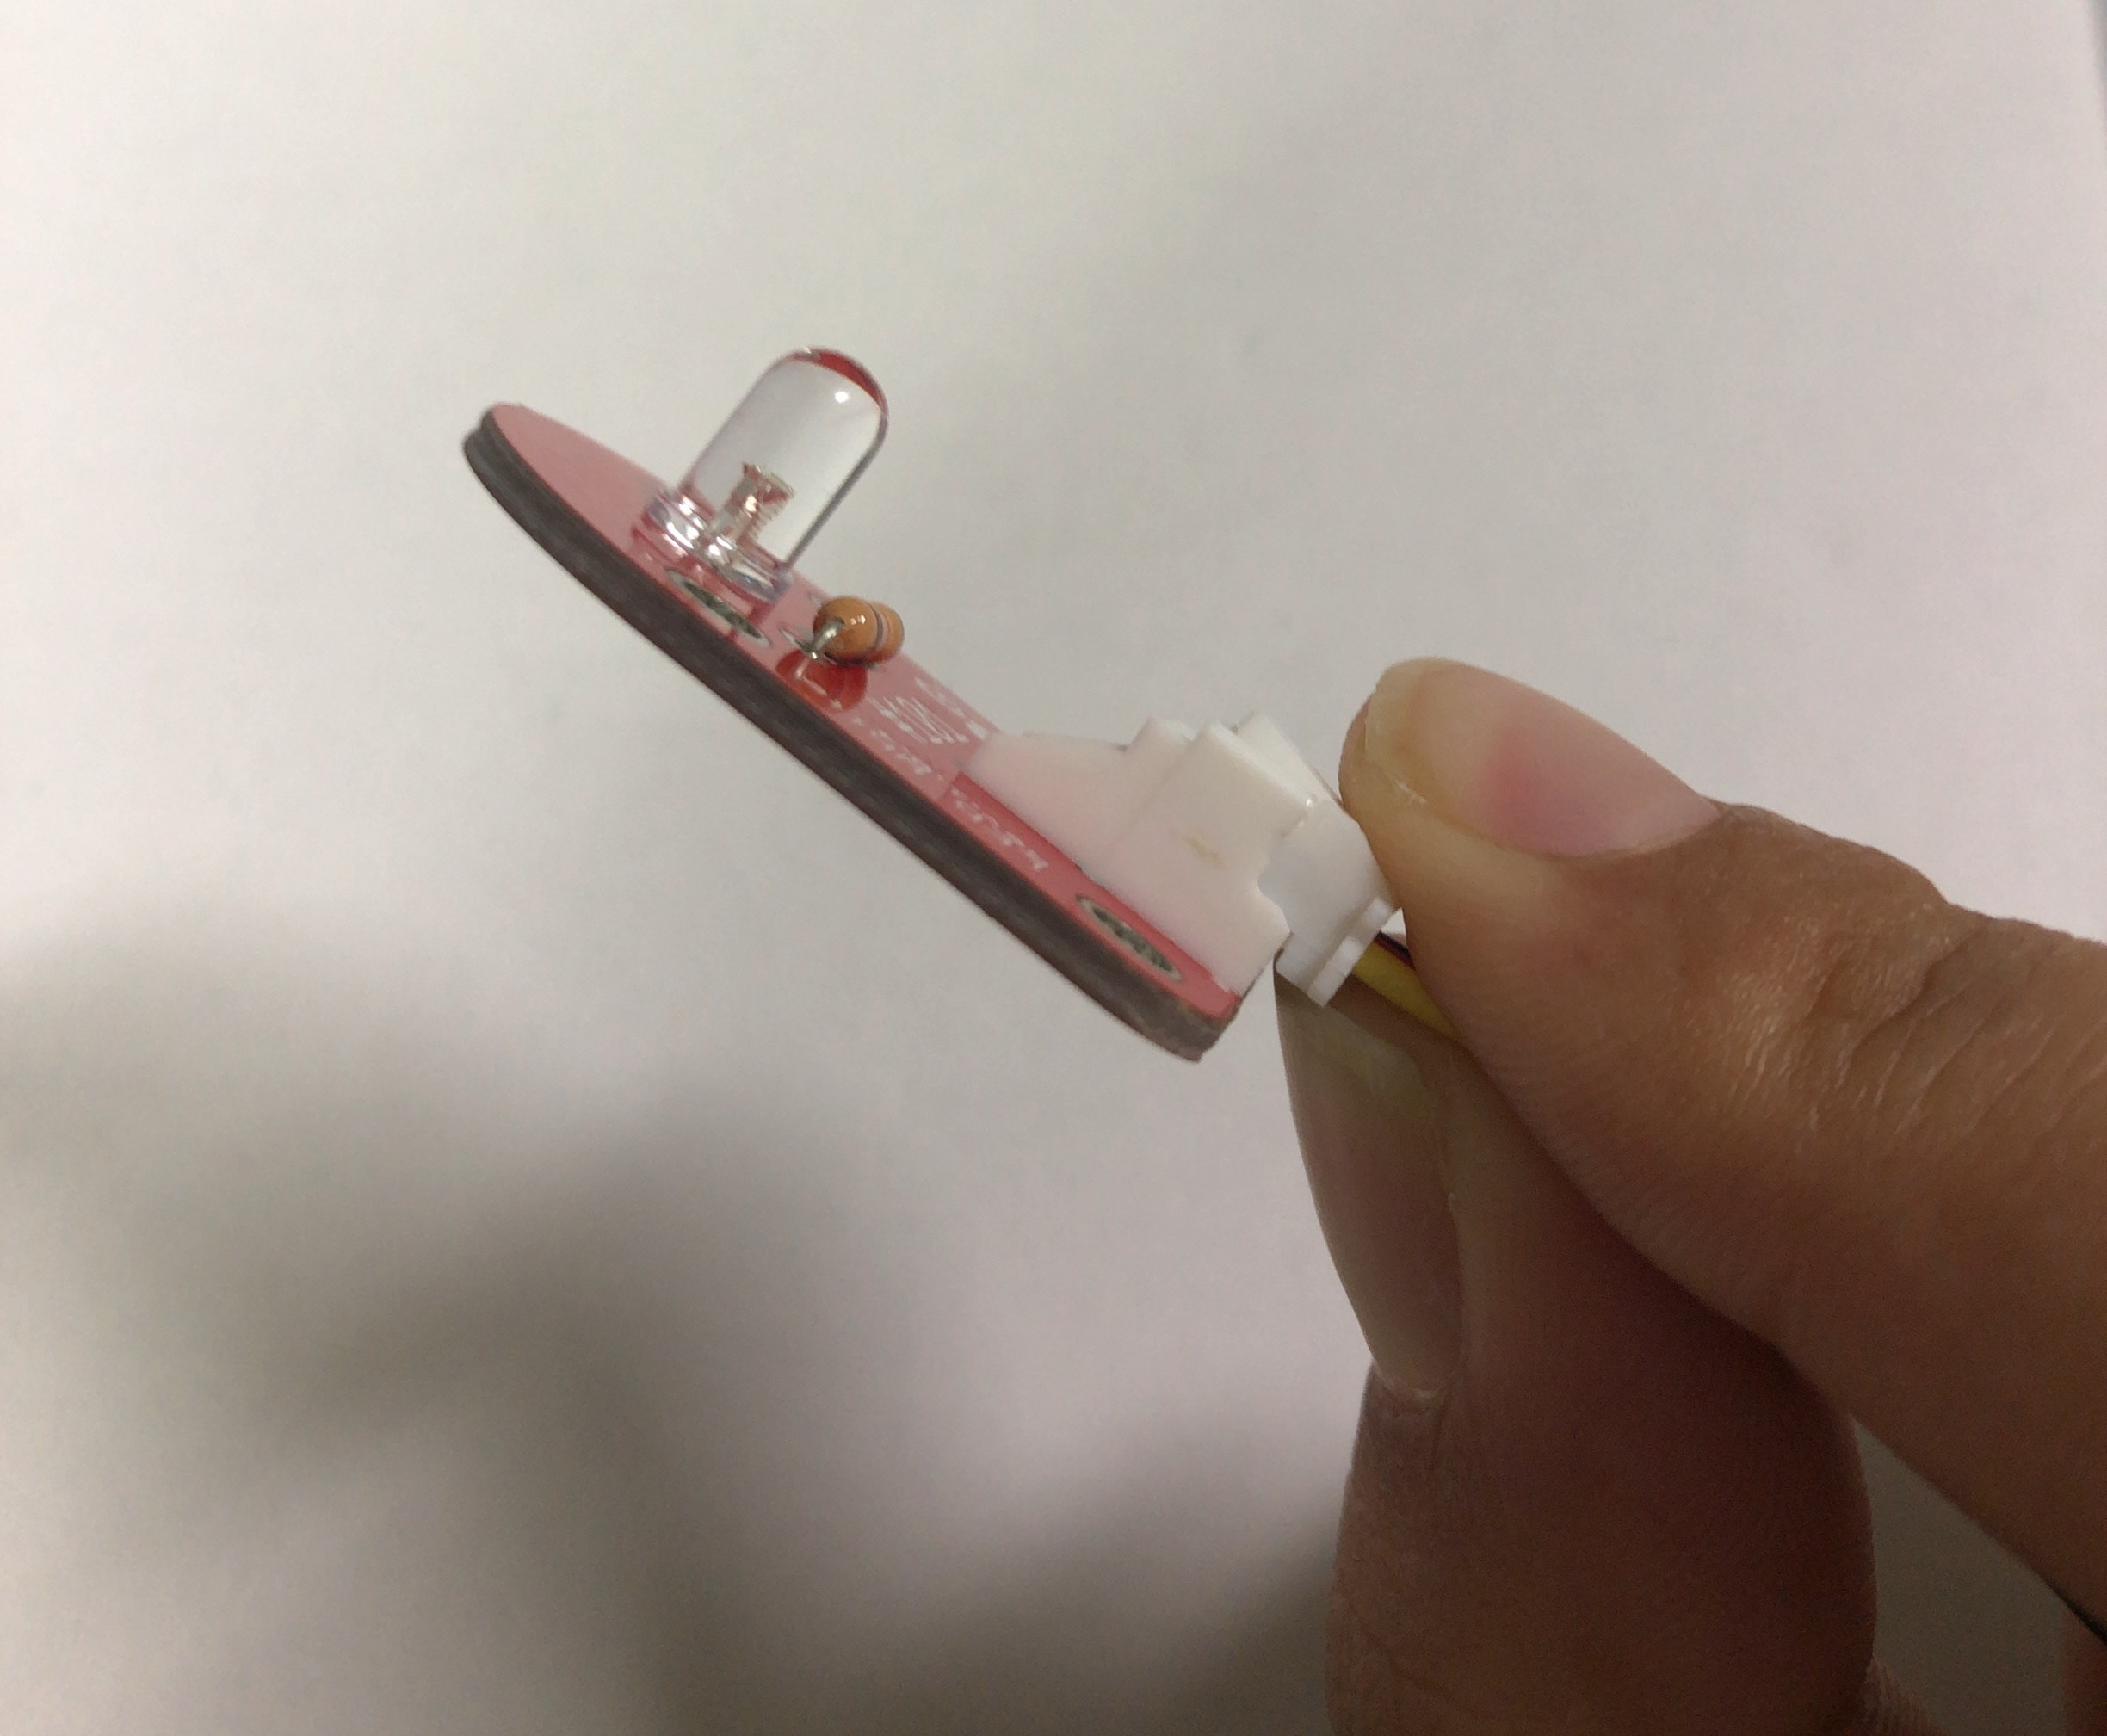
\includegraphics[width=7.281cm,height=5.997cm]{text05-img/text05-img010.jpg} \newline
図 \stepcounter{qwerty}{\theqwerty}:
ケーブルのツメの押し方}\end{minipage}
\\
\ 白い部分の下の方を押します。

~
 &
\ ツメの部分が少し浮いたら引きぬきましょう。抜けないときは無理に引っぱらず、周りの先生に聞きましょう。

~
\\
\end{supertabular}
\end{center}

\bigskip

{\bfseries
問題 5-\stepcounter{qwertya}{\theqwertya}}

Raspberry
PiとLEDを上記の手順を見ながらつなげてみましょう。


\bigskip

\clearpage\subsection[入力そうち、出力そうち]{\rmfamily
入力そうち、出力そうち}
入力そうちとはコンピュータに信号を送るためのものです。今回使う入力そうちはボタン、スイッチ、リミットスイッチ、傾斜(けいしゃ)センサー、照度(しょうど)センサー、距離(きょり)センサー、圧力(あつりょく)センサー、ボリュームがあります。逆に、出力そうちとはコンピュータから信号を受け取るためのものです。今回使う出力そうちはLED、振動子(しんどうし)、ゆうきELディスプレイがあります。


\bigskip

{\bfseries
問題 5-\stepcounter{qwertya}{\theqwertya}}

{\mdseries
入力そうち、出力そうちの違いを書きましょう。}

\begin{enumerate}
\item[] 
\bigskip
\end{enumerate}
\begin{enumerate}
\item[]
答え.                             


\bigskip
\end{enumerate}
\subsection[]{\rmfamily }
\clearpage\subsection[ピン番号、ケーブル]{\rmfamily
ピン番号、ケーブル}
FaBoのシールドにはブリックとRaspberry
Piを繋ぐためのピンがあります。ピンにはGPIO、A、I2Cがあります。下の表のように使い方が分けられているので、間違えないように気をつけましょう。

%\begin{figure}
\centering
\begin{minipage}{13.644cm}

\begin{minipage}{9.823cm}
 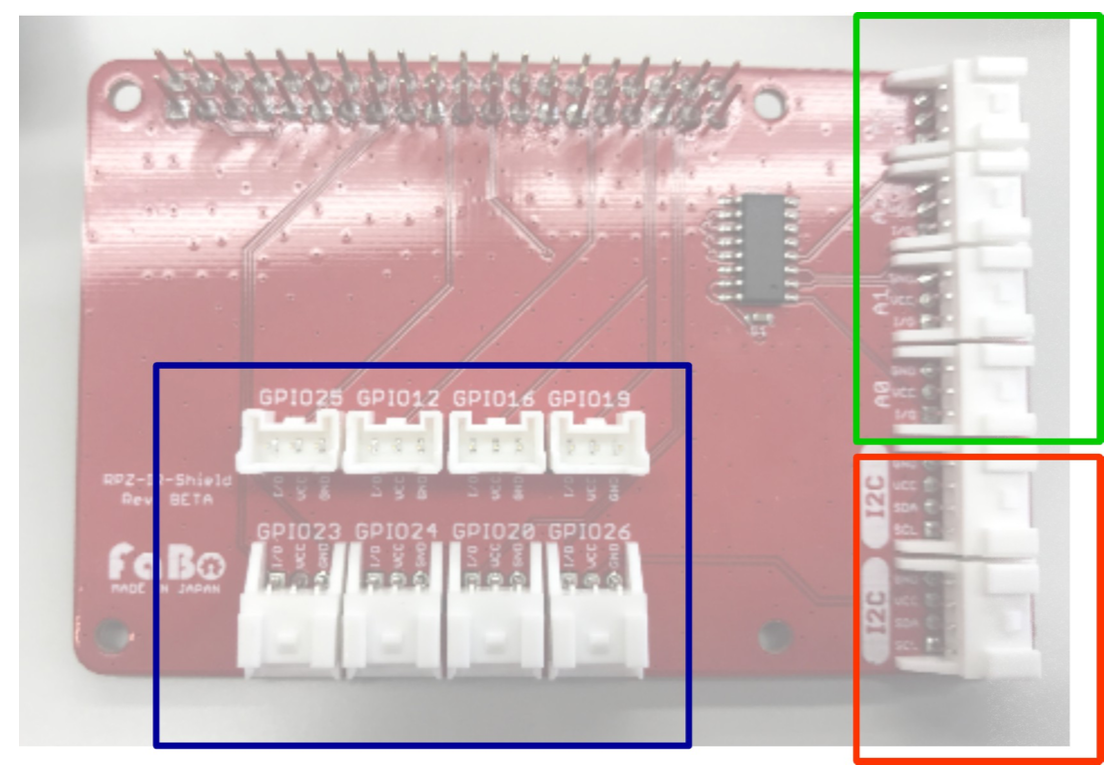
\includegraphics[width=9.823cm,height=6.036cm]{text05-img/text05-img011.png} \newline


図 \stepcounter{qwerty}{\theqwerty}: Faboシールドのピンはいち
\end{minipage}\begin{minipage}{3.019cm}
\textcolor[rgb]{0.8,0.0,0.0}{赤}:I2C
\end{minipage}\begin{minipage}{3.603cm}
\textcolor[rgb]{0.0,0.2,0.0}{緑}:A
\end{minipage}\end{minipage}
%\end{figure}


%\begin{figure}
\centering
\begin{minipage}{3.112cm}
\textcolor[rgb]{0.2,0.2,1.0}{青}:GPIO


\bigskip
\end{minipage}
%\end{figure}
\begin{center}
\tablefirsthead{}
\tablehead{}
\tabletail{}
\tablelasttail{}
\begin{supertabular}{|m{2.3009999cm}|m{14.304cm}|}
\hline
\centering GPIO 12 &
ボタンやスイッチなどのデジタル用のピン\\\hline
\centering GPIO 16 &
\\\hline
\centering GPIO 19 &
\\\hline
\centering GPIO 20 &
\\\hline
\centering GPIO 23 &
\\\hline
\centering GPIO 24 &
\\\hline
\centering GPIO 25 &
\\\hline
\centering GPIO 26 &
\\\hline
\centering A0 &
ボリュームや距離センサーなどのアナログ用のピン\\\hline
\centering A1 &
\\\hline
\centering A2 &
\\\hline
\centering A3 &
\\\hline
\centering I2C &
ゆうきELディスプレイのような特別な通信のためのピン\\\hline
\end{supertabular}
\end{center}

\bigskip

今まで使ってきたセンサーボードではGPIOの17,
18, 22,
24がLEDなど、あらかじめ番号が決められていました。しかしFaBoのGPIOはどの番号につなげても使えます。ただし、プログラムも番号に合わせて書く必要があります。


\bigskip

\clearpage
ケーブルは3ピンと4ピンの2種類があります。今回4ピンはゆうきELディスプレイで使います。



%\begin{figure}
\centering
\begin{minipage}{14.834cm}

\begin{minipage}{14.834cm}
{\upshape
 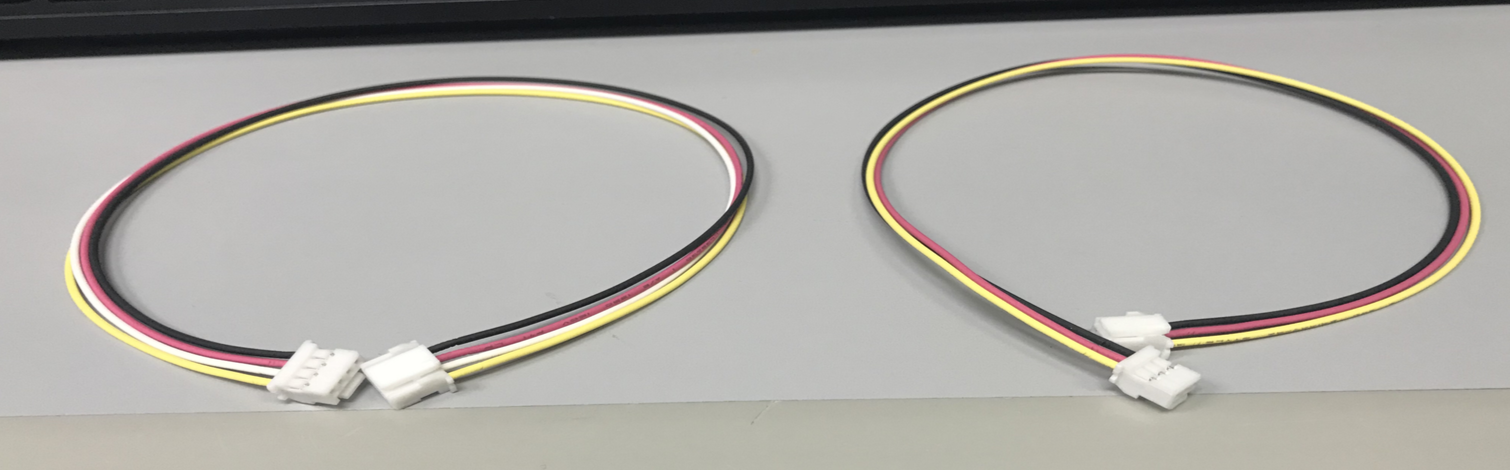
\includegraphics[width=14.834cm,height=4.616cm]{text05-img/text05-img012.png} \newline
図 \stepcounter{qwerty}{\theqwerty}:
4ピンケーブルと3ピンケーブル(全体)}
\end{minipage}\end{minipage}
%\end{figure}


%\begin{figure}
\centering
\begin{minipage}{14.811cm}


\begin{minipage}{6.9cm}
{\upshape
 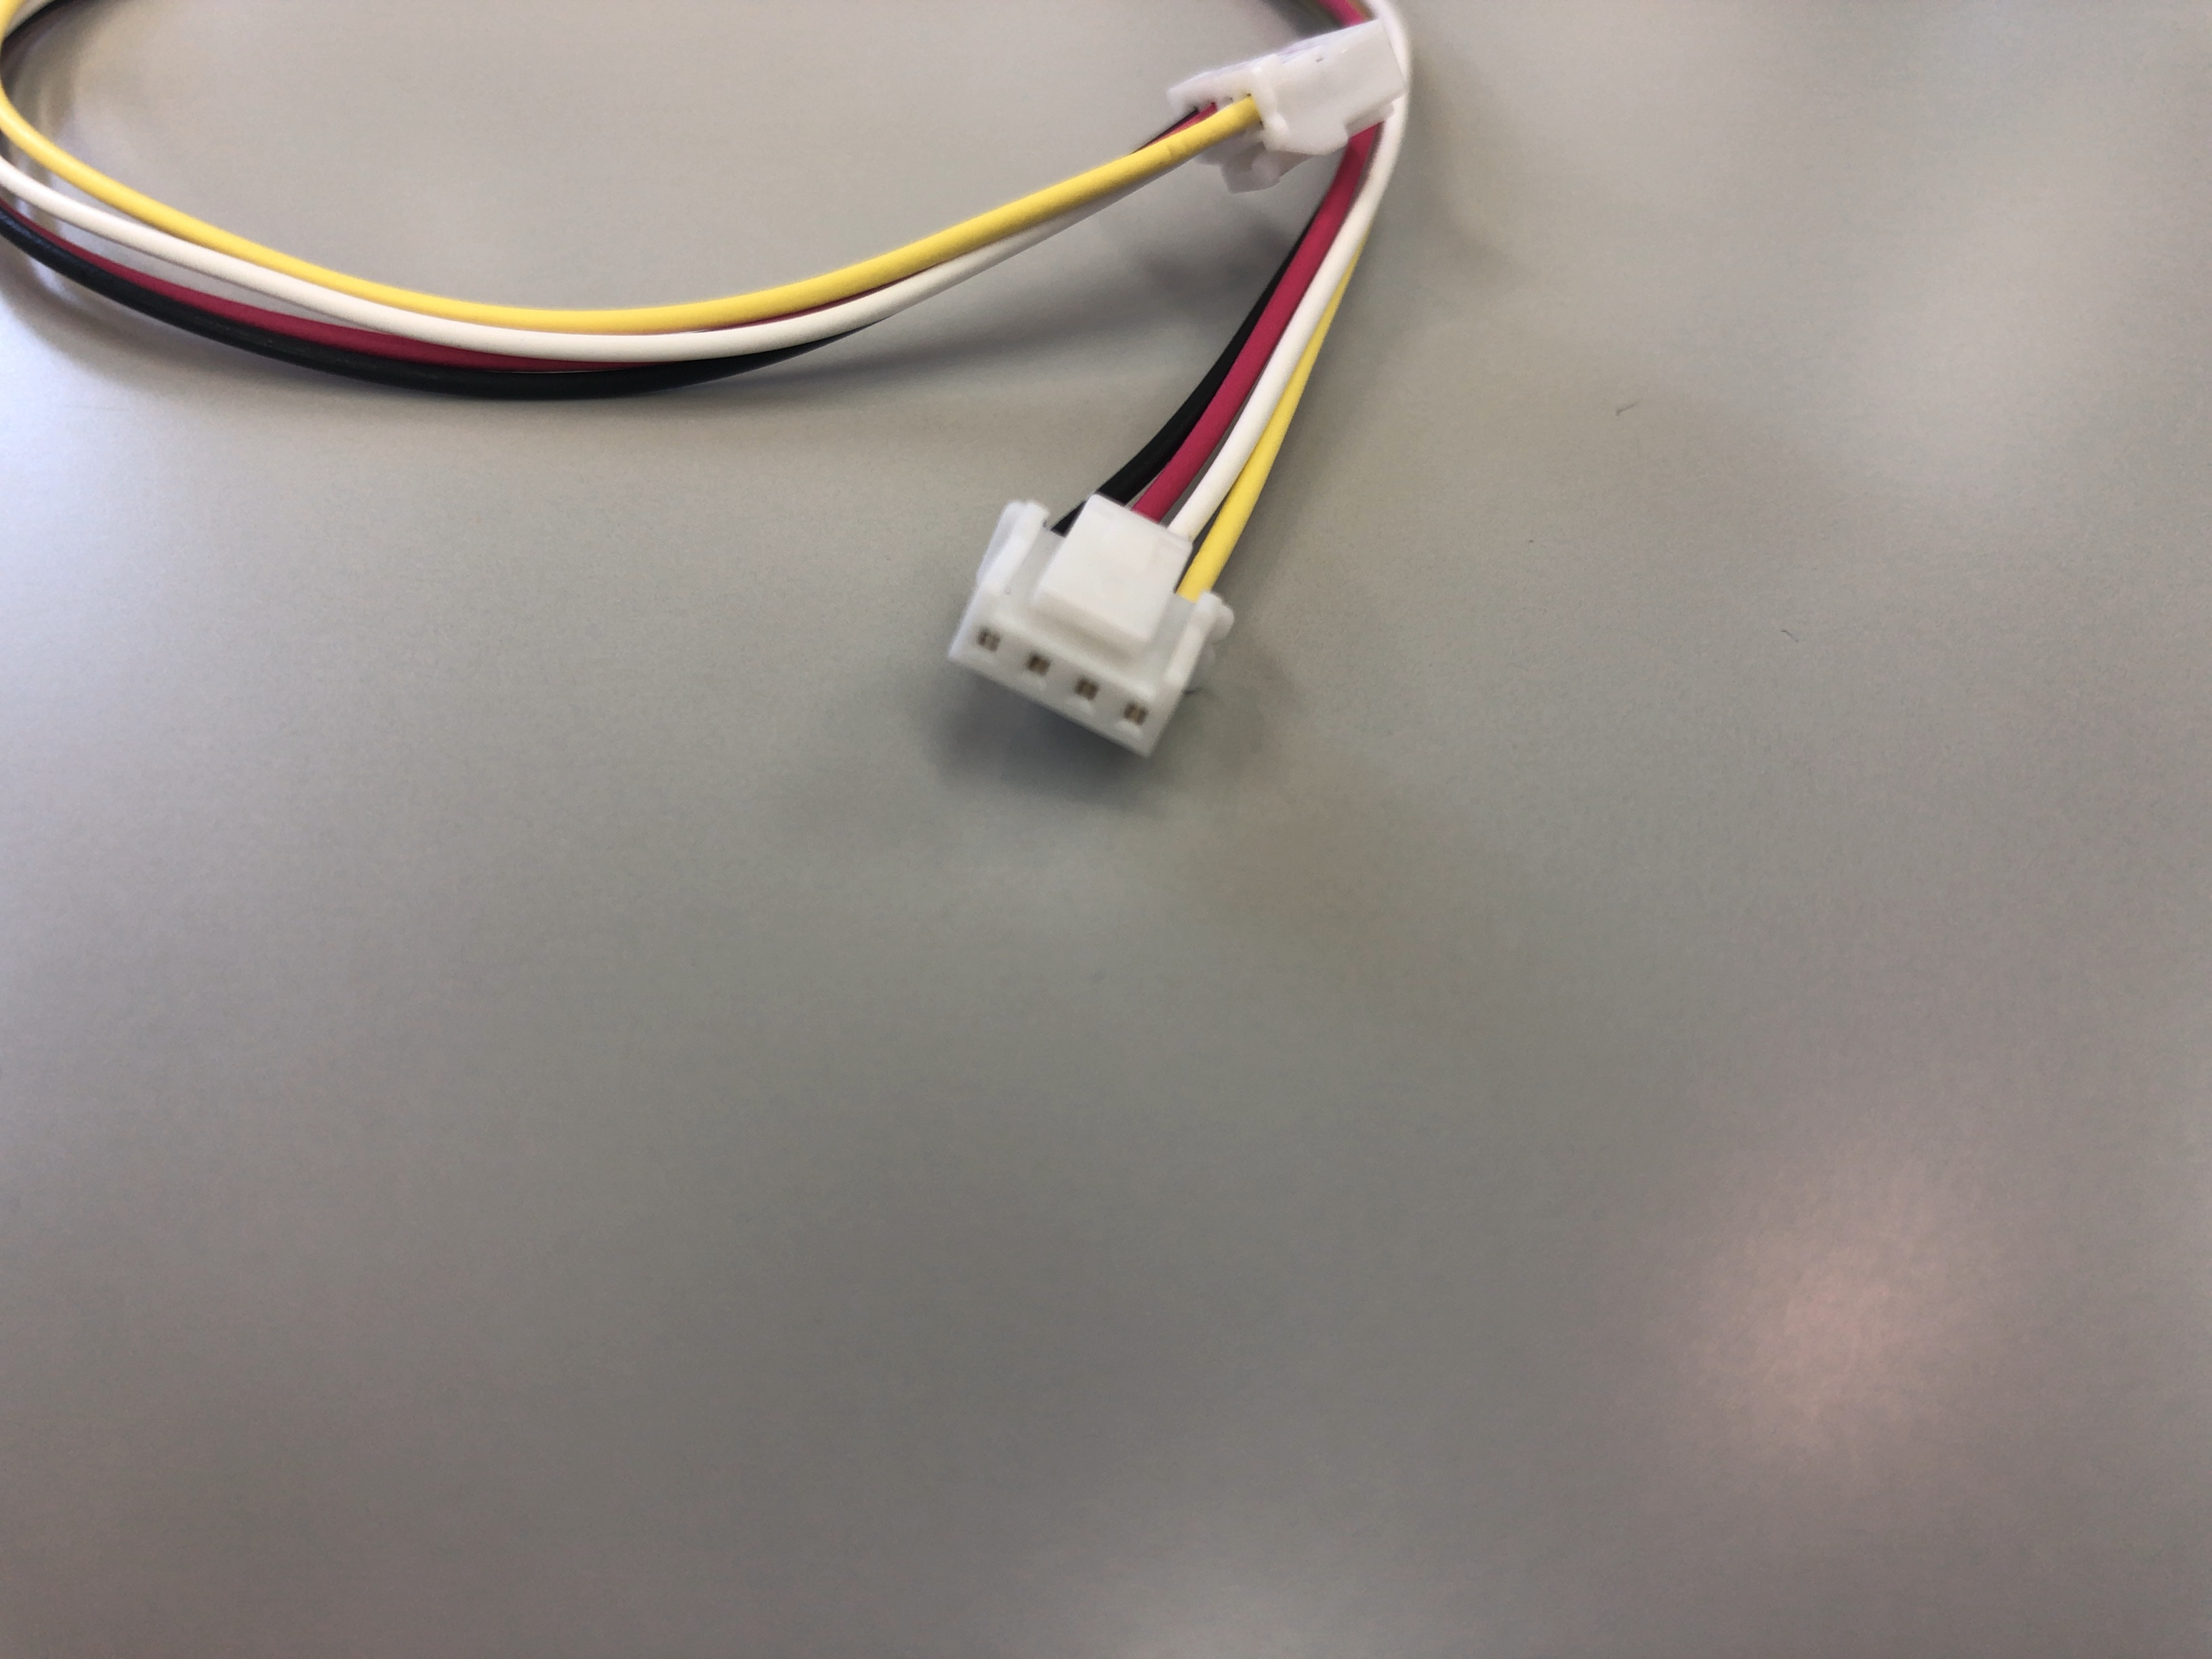
\includegraphics[width=6.9cm,height=5.175cm]{text05-img/text05-img013.jpg} \newline
図 \stepcounter{qwerty}{\theqwerty}:
3ピンケーブル(コネクタ)}
\end{minipage}\begin{minipage}{6.862cm}
{\upshape
 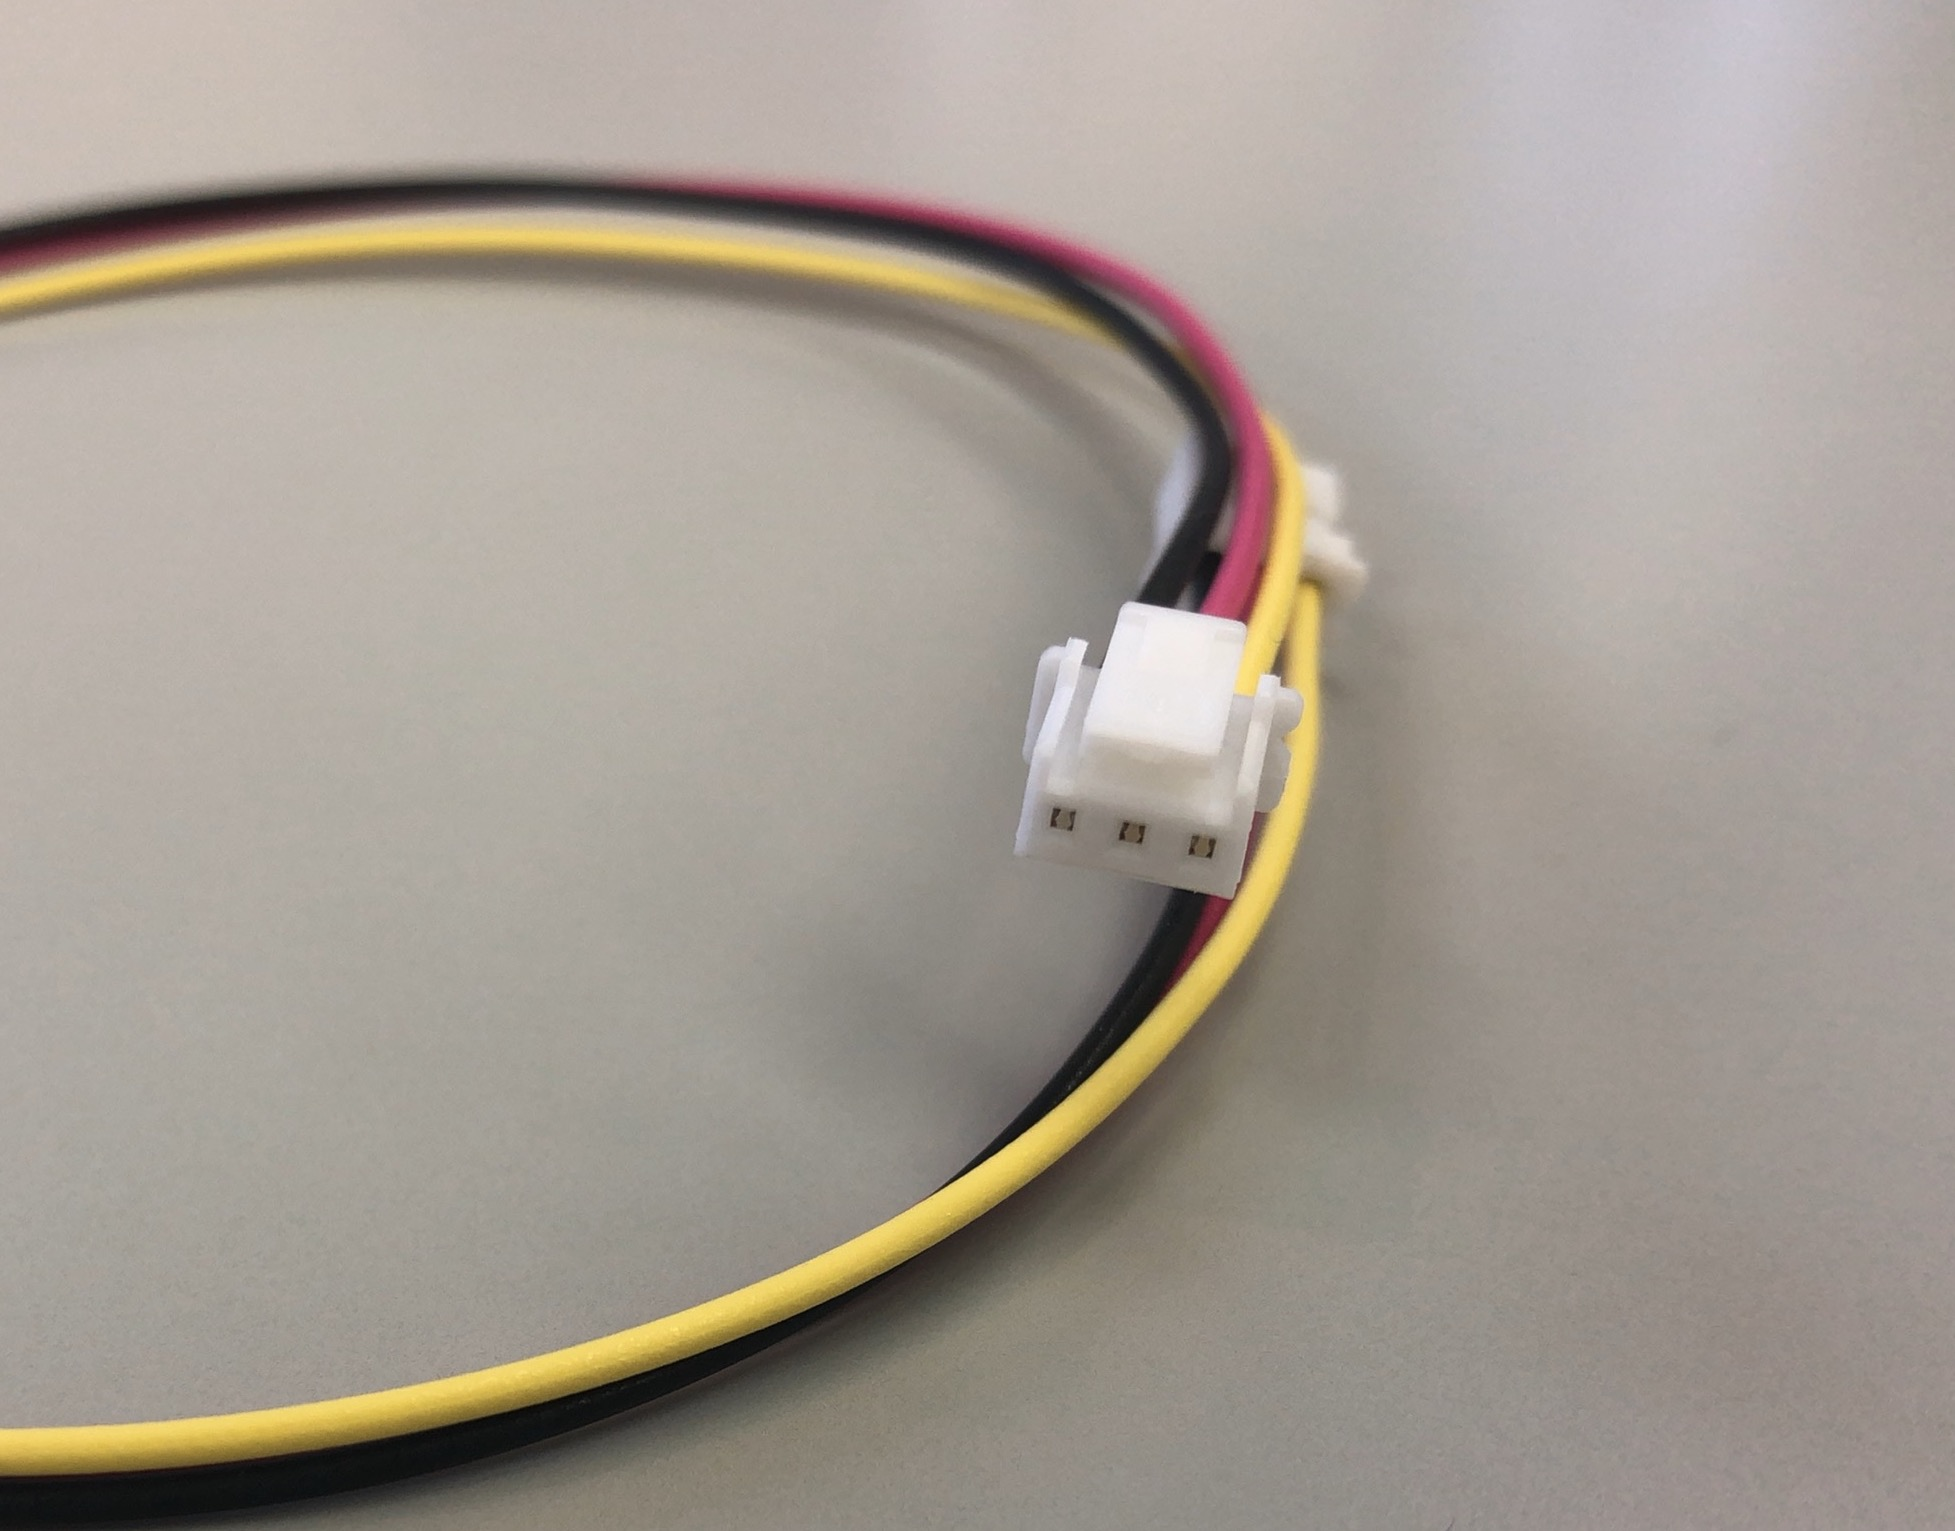
\includegraphics[width=6.569cm,height=5.145cm]{text05-img/text05-img014.jpg} \newline
図 \stepcounter{qwerty}{\theqwerty}:
3ピンケーブル(コネクタ)}
\end{minipage}
\bigskip


\bigskip


\bigskip


\bigskip


\bigskip


\bigskip
\end{minipage}
%\end{figure}
\clearpage\section[ブリックをつかってみよう]{\rmfamily
ブリックをつかってみよう}
\subsection[使うブリックについて]{\rmfamily
使うブリックについて}
子どもIT未来塾で使うブリックについて紹介します。ブリックには番号が書いてあるので、表で確認しながら間違えて使わないように注意しましょう。\ref{bkm:RefHeadingToc37441454936466}章のふろく:センサー紹介にはブリックについての詳しい説明が書いてあります。問題を解くときや自分で使ってみるときに参考にしましょう。


\bigskip

\begin{flushleft}
\tablefirsthead{}
\tablehead{}
\tabletail{}
\tablelasttail{}
\begin{supertabular}{|m{2.34cm}|m{2.658cm}|m{6.4090004cm}|m{3.672cm}|m{1.211cm}|}
\hline
{\mdseries 入出力} &
{\mdseries ブリック}

{\mdseries ブリック番号} &
{\mdseries 機能} &
{\mdseries 画像} &
{\mdseries 紹介ページ}\\\hline
{\mdseries デジタル出力そうち} &
{\mdseries LED}

{\mdseries \#101} &
\begin{itemize}
\item 順方向に電圧を加えると発光する
\item
プログラムでは値が1のとき光り、値が0のとき消える
\end{itemize}
 &
\centering
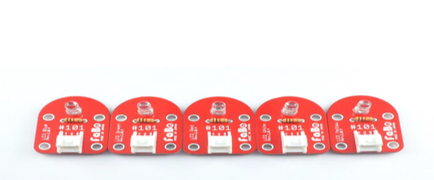
\includegraphics[width=3.699cm,height=2.092cm]{text05-img/text05-img015.png}
 &
{\mdseries \pageref{bkm:RefHeadingToc25509508239293}}\\\hline
 &
{\mdseries 振動子}

{\mdseries \#105} &
\begin{itemize}
\item 電圧が加わると振動する
\item
プログラムでは値が1のとき振動し、値が0のとき止まる
\end{itemize}
 &
\centering
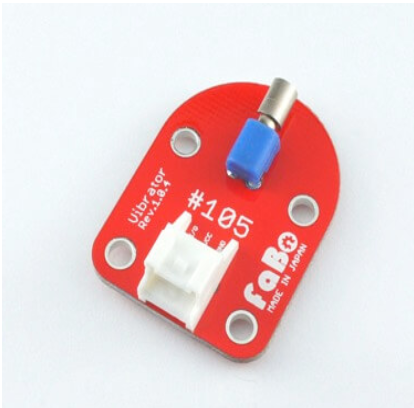
\includegraphics[width=2.616cm,height=2.577cm]{text05-img/text05-img016.png}
 &
{\mdseries \pageref{bkm:RefHeadingToc25513508239293}}\\\hline
{\mdseries デジタル入力そうち} &
{\mdseries ボタン}

{\mdseries \#103} &
\begin{itemize}
\item
押したり離したりしてONとOFFを切り替える。写真は黄色だが青や黒などの色もある。
\item
プログラムではボタンが押されている間1、ボタンが押されていないと0が入力される
\end{itemize}
 &
\centering
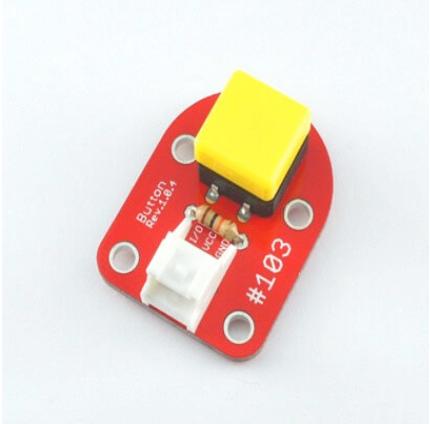
\includegraphics[width=2.411cm,height=2.378cm]{text05-img/text05-img005.png}
 &
{\mdseries \pageref{bkm:RefHeadingToc25515508239293}}\\\hline
 &
{\mdseries 傾斜センサー}

{\mdseries \#110} &
\begin{itemize}
\item
かたむいているかを調べることができる
\item
傾くと1,傾いていないと0の値が入力される
\end{itemize}
 &
{\mdseries    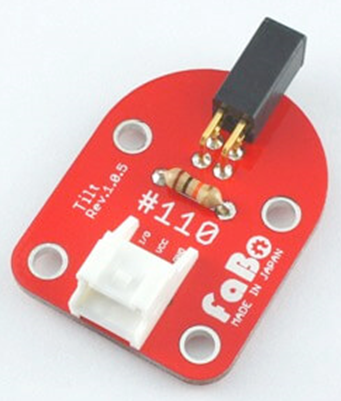
\includegraphics[width=2.491cm,height=2.233cm]{text05-img/text05-img017.png} } &
{\mdseries \pageref{bkm:RefHeadingToc25517508239293}}\\\hline
 &
{\mdseries スイッチ}

{\mdseries \#117} &
\begin{itemize}
\item
ボタンと似ているが、ONのまま、OFFのままにできる
\item
${\bullet}にスライドさせると$ON、${\circ}にスライドさせると$OFFになる
\item ONのときは1,OFFのときは0が入力される
\end{itemize}
 &
\centering
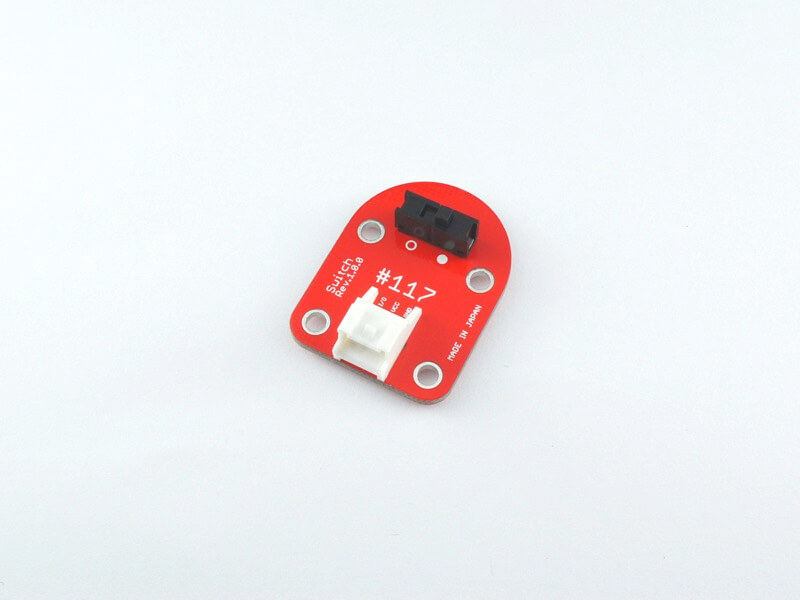
\includegraphics[width=2.394cm,height=2.31cm]{text05-img/text05-img018.jpg}
 &
{\mdseries \pageref{bkm:RefHeadingToc25519508239293}}\\\hline
 &
{\mdseries リミットスイッチ}

{\mdseries \#107} &
\begin{itemize}
\item
ボタンに似ている。銀の部分が押されているとON、押されていないとOFFになる
\item
スイッチはONのときは1,OFFのときは0が入力される
\end{itemize}
 &
\centering
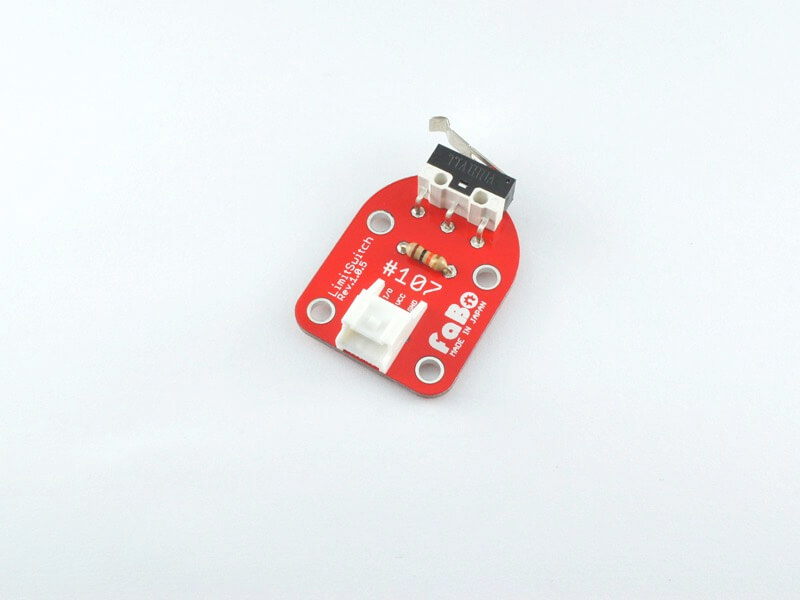
\includegraphics[width=2.426cm,height=2.8cm]{text05-img/text05-img019.jpg}
 &
{\mdseries \pageref{bkm:RefHeadingToc25709508239293}}\\\hline
{\mdseries アナログ入力そうち} &
{\mdseries 感圧センサー}

{\mdseries \#106} &
\begin{itemize}
\item
加えた力の大きさを調べることができる
\item
0〜1023の値が入力される。圧力が小さい時は値が大きく、圧力が大きい時は値が小さくなる。
\end{itemize}
 &
\centering
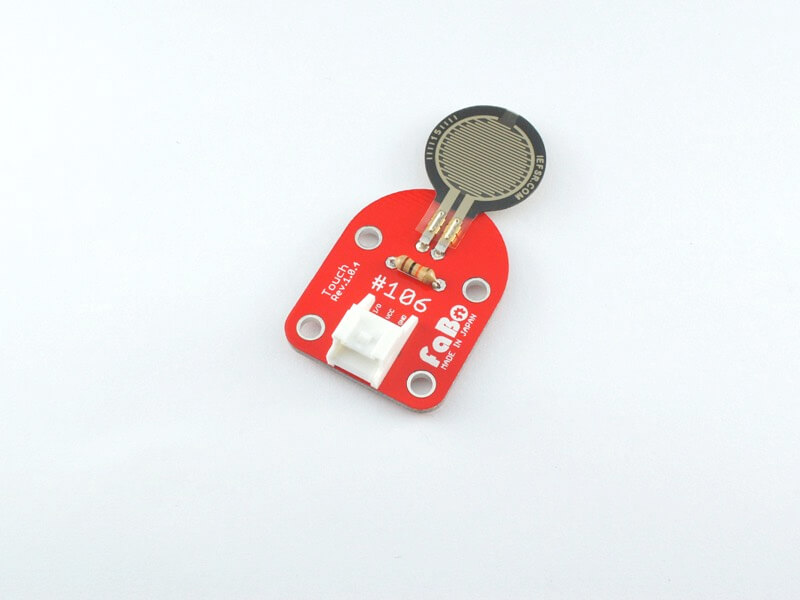
\includegraphics[width=2.92cm,height=2.627cm]{text05-img/text05-img020.jpg}
 &
{\mdseries \pageref{bkm:RefHeadingToc25711508239293}}\\\hline
 &
{\mdseries ボリューム}

{\mdseries \#104} &
\begin{itemize}
\item
じくをひねると電圧の大きさを変えることができる
\item
0〜1023の値が入力される。右に回すほど値が大きくなる。
\end{itemize}
 &
 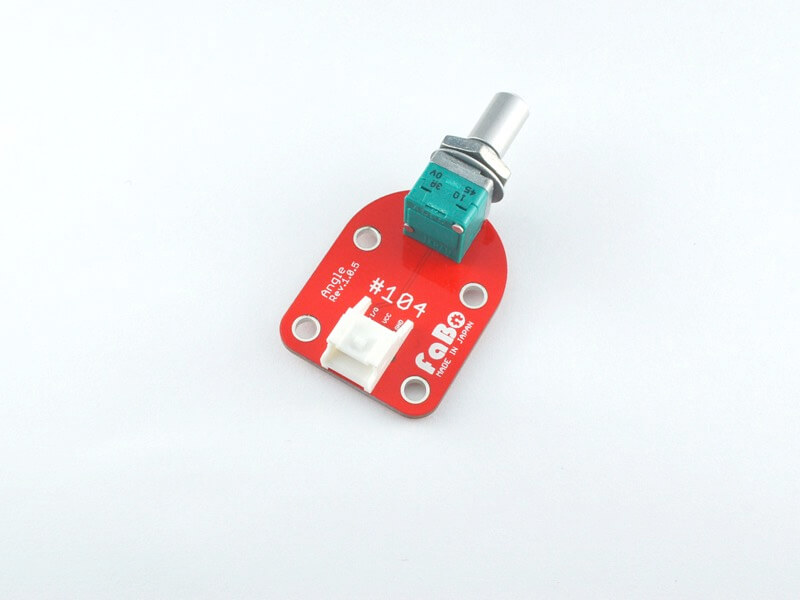
\includegraphics[width=6.858cm,height=5.131cm]{text05-img/text05-img021.jpg}  &
{\mdseries \pageref{bkm:RefHeadingToc25713508239293}}\\\hline
 &
{\mdseries 距離センサー}

{\mdseries \#116}

{\mdseries (番号は書いてありません)} &
\begin{itemize}
\item 距離を測ることができる
\item
0〜1023の値が入力される。距離に変換する必要がある。
\end{itemize}
 &
 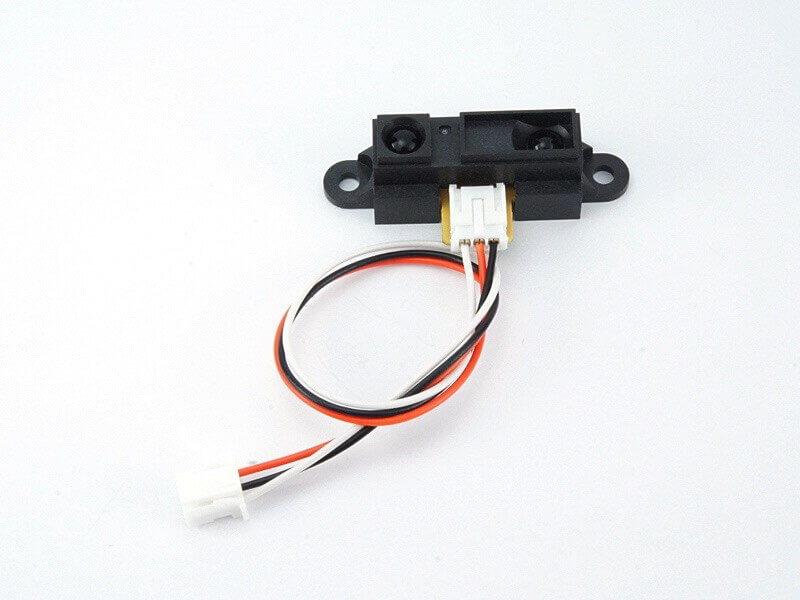
\includegraphics[width=3.678cm,height=2.736cm]{text05-img/text05-img022.jpg}  &
{\mdseries \pageref{bkm:RefHeadingToc5917367650265}}\\\hline
 &
{\mdseries 照度センサー}

{\mdseries \#109} &
\begin{itemize}
\item 明るさの変化を測ることができる
\item
0〜1023の値が入力される。暗いほど値が大きくなる。
\end{itemize}
 &
\centering
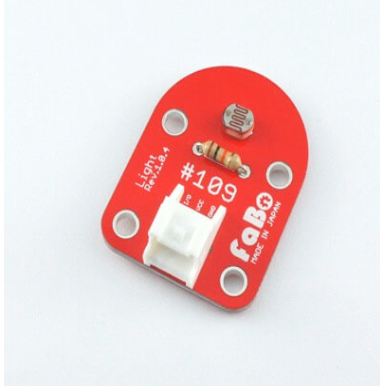
\includegraphics[width=2.399cm,height=2.425cm]{text05-img/text05-img023.png}
 &
{\mdseries \pageref{bkm:RefHeadingToc25715508239293}}\\\hline
{\mdseries その他} &
{\mdseries ゆうきELディスプレイ}

{\mdseries \#214} &
\begin{itemize}
\item
文字を画面に表示させることができる(アルファベットと記号のみ)
\item oled ``文字''で表示する
\end{itemize}
~
 &
\centering
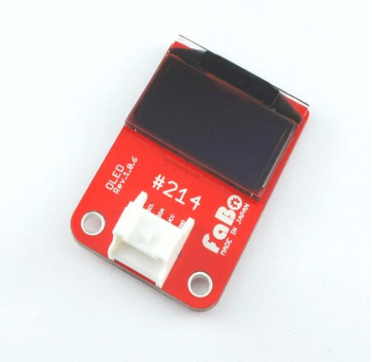
\includegraphics[width=2.886cm,height=2.808cm]{text05-img/text05-img024.png}
 &
{\mdseries \pageref{bkm:RefHeadingToc25717508239293}}\\\hline
\end{supertabular}
\end{flushleft}

\bigskip

\clearpage
\bigskip

\subsection{デジタル出力そうちを使ってみよう}
デジタル出力そうちをHSPで使ってみましょう。GPIO23にLED(\#101)をつけてください。HSPスクリプトエディタで/home/pi/ome/05/digout.hspを開いて、実行してみましょう。

{\centering
\begin{minipage}{2.404cm}
\begin{minipage}{2.404cm}
{\upshape
 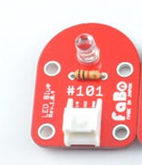
\includegraphics[width=2.404cm,height=2.794cm]{text05-img/text05-img025.png} \newline
図 \stepcounter{qwerty}{\theqwerty}: LED}
\end{minipage}
\end{minipage}   \begin{minipage}{10.442cm}
\begin{minipage}{12.938cm}
{\upshape
 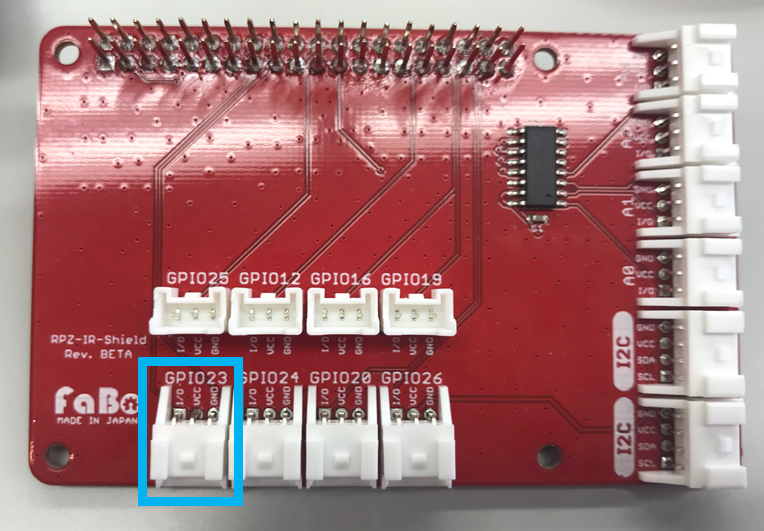
\includegraphics[width=12.938cm,height=8.992cm]{text05-img/text05-img026.png} \newline
図 \stepcounter{qwerty}{\theqwerty}: GPIO23}
\end{minipage}
\end{minipage}
\par}

GPIO12,GPIO16,GPIO19,GPIO20,GPIO24,GPIO25,GPIO26はデジタル入出力そうち用のピンです。センサーボードで使ったgpio命令で使うことができます。\texttt{\textbf{gpio
GPIOピン番号,値}}でブリックを動かしたり、止めたりできます。

%\begin{figure}
\centering
\begin{minipage}{\textwidth}
{\ttfamily\bfseries
\#include {\textquotedbl}hsp3dish.as{\textquotedbl}}

\begin{minipage}{17.006cm}
{\ttfamily\bfseries
\ \ gpio 23,1\ \ \textcolor[rgb]{0.0,0.0,0.6}{;GPIO23のセンサーを動かす}}

{\ttfamily\bfseries
\ \ wait 100}

{\ttfamily\bfseries
\ \ gpio 23,0\ \ \textcolor[rgb]{0.0,0.0,0.6}{;GPIO23のセンサーを止める}}
\end{minipage}\begin{minipage}{16.501cm}
{\ttfamily\bfseries
[Warning: Draw object ignored][Warning: Draw object ignored]\ \ redraw 0}

{\ttfamily\bfseries
\ \ font {\textquotedbl}{\textquotedbl},20}

{\ttfamily\bfseries
\ \ pos 20,20}

{\ttfamily\bfseries
\ \ mes
{\textquotedbl}センサーが動いたり止まったりします{\textquotedbl}}

{\ttfamily\bfseries
\ \ redraw 1}
\end{minipage}{\ttfamily\bfseries
\#include {\textquotedbl}rpz-gpio.as{\textquotedbl}}


\bigskip

{\ttfamily\bfseries
*main}

{\ttfamily\bfseries
\ \ wait 100}

{\ttfamily\bfseries
\ \ goto *main}

{\mdseries
リスト \stepcounter{List}{\theList}: digout.hsp}
\end{minipage}
%\end{figure}
%\begin{figure}
\centering
\begin{minipage}{\textwidth}
{\ttfamily\bfseries
\#include {\textquotedbl}hsp3dish.as{\textquotedbl}}

\begin{minipage}{17.006cm}
{\ttfamily\bfseries
\ \ gpio 23,1\ \ \textcolor[rgb]{0.0,0.0,0.6}{;GPIO23のブリックを動かす}}

{\ttfamily\bfseries
\ \ wait 100}

{\ttfamily\bfseries
\ \ gpio 23,0\ \ \textcolor[rgb]{0.0,0.0,0.6}{;GPIO23のブリックを止める}}
\end{minipage}\begin{minipage}{16.501cm}
{\ttfamily\bfseries
[Warning: Draw object ignored][Warning: Draw object ignored]\ \ redraw 0}

{\ttfamily\bfseries
\ \ font {\textquotedbl}{\textquotedbl},20}

{\ttfamily\bfseries
\ \ pos 20,20}

{\ttfamily\bfseries
\ \ mes
{\textquotedbl}センサーが動いたり止まったりします{\textquotedbl}}

{\ttfamily\bfseries
\ \ redraw 1}
\end{minipage}{\ttfamily\bfseries
\#include {\textquotedbl}rpz-gpio.as{\textquotedbl}}


\bigskip

{\ttfamily\bfseries
*main}

{\ttfamily\bfseries
\ \ wait 100}

{\ttfamily\bfseries
\ \ goto *main}

{\mdseries
リスト \stepcounter{List}{\theList}: digout.hsp}
\end{minipage}
%\end{figure}
{\mdseries
digout.hspはデジタル出力そうち用のプログラムです。LEDや振動子に使うことができます。}


\bigskip

\texttt{\textbf{gpio
GPIOピン番号,0}}でブリックを動かします。\newline
\texttt{\textbf{gpio
GPIOピン番号,1}}でブリックを止めます。


\bigskip

{\bfseries
問題 5-\stepcounter{qwertya}{\theqwertya}}

digout.hspのgpio 23,1をgpio 25,1に。gpio 23,0をgpio
25,0に変えましょう。LEDをGPIO25につけて、プログラムを実行しましょう。\newline


{\bfseries
問題 5-\stepcounter{qwertya}{\theqwertya}}

{\mdseries
LEDを振動子(\#105)に変えて、digout.hspを実行しましょう。\newline
}


\bigskip

\clearpage\subsection{デジタル入力そうちを使ってみよう}
デジタル入力そうちをHSPで使ってみましょう。GPIO24にボタン(\#103)をつけてください。HSPスクリプトエディタで/home/pi/ome/05/digin.hspを開いて実行してみましょう。

{\centering
\begin{minipage}{2.845cm}
\begin{minipage}{2.845cm}
{\upshape
 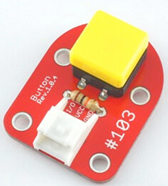
\includegraphics[width=2.845cm,height=3.149cm]{text05-img/text05-img027.png} \newline
図 \stepcounter{qwerty}{\theqwerty}: ボタン}
\end{minipage}
\end{minipage}   \begin{minipage}{10.112cm}
\begin{minipage}{12.938cm}
{\upshape
 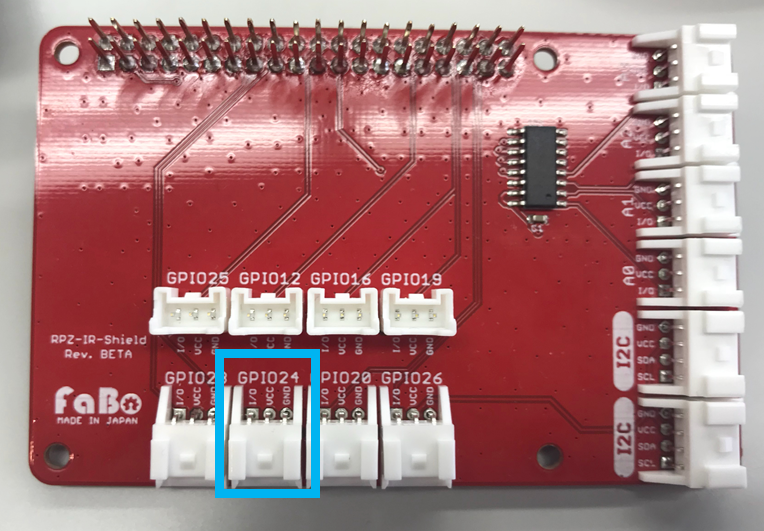
\includegraphics[width=12.938cm,height=8.992cm]{text05-img/text05-img028.png} \newline
図 \stepcounter{qwerty}{\theqwerty}: GPIO24}
\end{minipage}
\end{minipage}
\par}



%\begin{figure}
\centering
\begin{minipage}{17.006cm}
{\ttfamily\bfseries
\#include {\textquotedbl}hsp3dish.as{\textquotedbl}\newline
\#include {\textquotedbl}rpz-gpio.as{\textquotedbl}\newline
\newline
*main\newline
 }

\begin{minipage}{16.48cm}
{\ttfamily\bfseries
*digital\_off\newline
\ \ gpio 17, 0\newline
\ \ wait 10\newline
\ \ goto *main }
\end{minipage}\begin{minipage}{16.501cm}
{\ttfamily\bfseries
[Warning: Draw object ignored]*digital\_on\newline
\ \ gpio 17, 1\newline
\ \ wait 10\newline
\ \ goto *main}
\end{minipage}\begin{minipage}{16.538cm}
{\ttfamily\bfseries
\ \ if gpioin(24)=1 : goto
*digital\_on\ \ \textcolor[rgb]{0.0,0.0,0.6}{;GPIO24の値が1のとき*digital\_onを実行する}\newline
\ \ goto *digital\_off}
\end{minipage}\begin{minipage}{16.485cm}
{\ttfamily\bfseries
[Warning: Draw object ignored][Warning: Draw object ignored]\ \ redraw 0\newline
\ \ pos 30,30\newline
\ \ mes
{\textquotedbl}デジタル入力そうちでLEDを光らせよう{\textquotedbl}\newline
\ \ redraw 1}
\end{minipage}{\mdseries
リスト \stepcounter{List}{\theList}: digin.hsp}
\end{minipage}
%\end{figure}

\bigskip


\bigskip

[Warning: Draw object ignored]


\bigskip


\bigskip


\bigskip


\bigskip


\bigskip


\bigskip

\clearpage
digin.hspはデジタル入力用のプログラムです。ボタン、スイッチ、リミットスイッチ、傾斜センサーに使うことができます。

\texttt{\textbf{gpioin(GPIO番号)}}でデジタル入力を受け取ることができます。

{\ttfamily\bfseries
if gpioin(24)=1 : goto
*digital\_onでデジタル入力があったとき*digital\_onに移動します。*digital\_onでは
gpio 17,
1でLEDを光らせています。デジタル入力がないときは
goto *digital\_offで*digital\_offに移動します。*digital\_offでは gpio
17, 0でLEDを消しています。}


\bigskip

\textbf{問題 5{}-\stepcounter{qwertya}{\theqwertya}}

ボタン(\#103)をGPIO24につなげて上記のプログラムdigin.hspを実行してみましょう。\newline


\textbf{問題 5{}-\stepcounter{qwertya}{\theqwertya}}

スイッチ(\#117)をGPIO24につなげてdigin.hspを実行してみましょう\newline


\textbf{問題 5{}-\stepcounter{qwertya}{\theqwertya}}

リミットスイッチ(\#107)をGPIO24につなげてdigin.hspを実行してみましょう\newline


\textbf{問題 5{}-\stepcounter{qwertya}{\theqwertya}}

傾斜センサー(\#110)をGPIO24につなげてdigin.hspを実行してみましょう\newline


\textbf{問題 5{}-\stepcounter{qwertya}{\theqwertya}}

ボタンをつなげるピンを変えてみましょう。GPIO20にボタン(\#103)をつけましょう。\newline
gpioin(24)をgpioin(20)に変えましょう。digin.hspを実行してみましょう。\newline


\textbf{チャレンジ問題 5-\stepcounter{qwertyb}{\theqwertyb}}

時間があまったら挑戦してみましょう。\newline
ボタン(\#103)をGPIO26、LED(\#101)をGPIO20につなげます。ボタンを押している間LEDが光るようにdigin.hspを書きかえましょう。\newline


\textbf{チャレンジ問題 5-\stepcounter{qwertyb}{\theqwertyb}}

時間があまったら挑戦してみましょう。\newline
ボタンを押して、LEDのONとOFFが切りかわるように、digin.hspを書きかえましょう。\newline


\clearpage\subsection{アナログ入力そうちを使ってみよう}
アナログ入力そうちをHSPで使ってみましょう。アナログ入力そうちをA0につなげてください。

{\centering \begin{minipage}{8.851cm}
{\upshape
 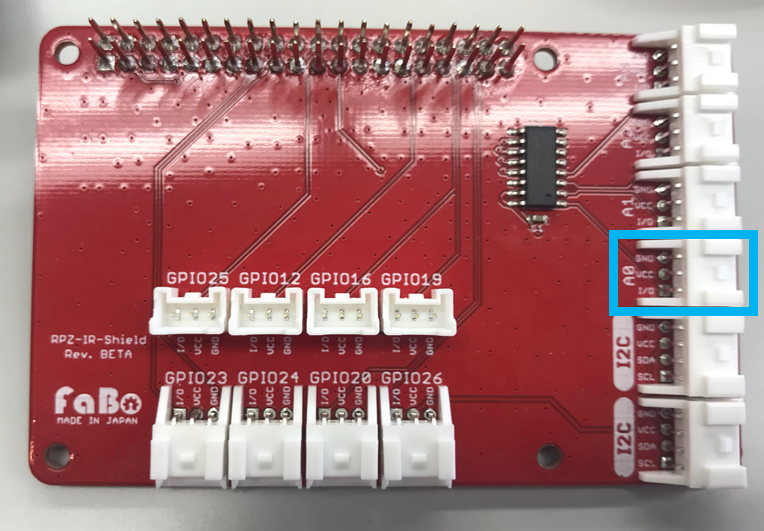
\includegraphics[width=8.851cm,height=6.075cm]{text05-img/text05-img029.png} \newline
図 \stepcounter{qwerty}{\theqwerty}: アナログ入力A0}
\end{minipage}\par}
{\mdseries
HSPスクリプトエディタで/home/pi/ome/05/anain.hspを開いて実行してみましょう。}

anain.hspはアナログ入力そうち用のプログラムです。アナログ入力にはA0,A1,A2,A3のピンを使います。感圧センサー、ボリューム、距離センサー、照度センサーを使うことができます。

%\begin{figure}
\centering
\begin{minipage}{17.006cm}
{\ttfamily\bfseries
\#include {\textquotedbl}hsp3dish.as{\textquotedbl}}

{\ttfamily\bfseries
\#include {\textquotedbl}rpz-gpio.as{\textquotedbl}}


\bigskip

{\ttfamily\bfseries
spiopen 0\ \ \textcolor[rgb]{0.0,0.0,0.6}{;SPIチャンネルを開く}}


\bigskip

{\ttfamily\bfseries
*main}

{\ttfamily\bfseries
\ \ data =
spiget(0,0)\ \ \textcolor[rgb]{0.0,0.0,0.6}{;SPIを使ってデータを受け取る}}

{\ttfamily\bfseries
\ \ res = {\textquotedbl}結果 : {\textquotedbl}+data+{\textquotedbl}{\textbackslash}n{\textquotedbl}}


\bigskip

{\ttfamily\bfseries
\ \ redraw 0}

{\ttfamily\bfseries
\ \ pos 20,20}

{\ttfamily\bfseries
\ \ font {\textquotedbl}{\textquotedbl},30}

{\ttfamily\bfseries
\ \ mes res}

{\ttfamily\bfseries
\ \ redraw 1}


\bigskip

{\ttfamily\bfseries
\ \ wait 10}

{\ttfamily\bfseries
\ \ goto *main}


\bigskip

{\ttfamily\bfseries
spiclose 0\ \ \textcolor[rgb]{0.0,0.0,0.6}{;SPIチャンネルを閉じる}}

{\mdseries
リスト \stepcounter{List}{\theList}: anain.hsp}
\end{minipage}
%\end{figure}

\bigskip

\clearpage
アナログ入力そうちから入力を受け取るときにSPI(Serial
Peripheral
Interface)という方法を使っています。\texttt{\textbf{spiopen
0}}命令を使ってラズベリーパイとアナログ入力そうちをつなげます。\texttt{\textbf{spiclose
0}}命令を使ってラズベリーパイとアナログ入力そうちのつながりを切ります。

アナログ入力は\texttt{\textbf{spiget(ピン番号,0)}}で値を受け取ります。ピン番号はブリックがつながっている番号です。入力される値は0〜1023までの数字になります。詳しいアナログ入力そうちの使い方は\pageref{bkm:RefHeadingToc4569508239293}ページから見てみましょう。


\bigskip

{\bfseries
問題 5-\stepcounter{qwertya}{\theqwertya}}

{\mdseries
感圧センサー(\#106)をA0につなげて上記のanain.hspを実行してみましょう。感圧センサーにさわる強さによって、画面の数字が変わります。}


\bigskip

{\bfseries
問題 5-\stepcounter{qwertya}{\theqwertya}}

{\mdseries
ボリューム(\#104)をA0につなげてanain.hspを実行してみましょう。ボリュームを動かすと、画面の数字が変わります。\newline
}

{\bfseries
問題 5-\stepcounter{qwertya}{\theqwertya}}

{\mdseries
照度センサー(\#109)をA0につなげてanain.hspを実行してみましょう。明るさによって、画面の数字が変わります。\newline
}

{\bfseries
問題 5-\stepcounter{qwertya}{\theqwertya}}

{\mdseries
\texttt{\textbf{spiget(0,0)}}を\texttt{\textbf{spiget(1,0)}}に変えましょう。A1にアナログ入力そうちをつなぎましょう。anain.hspを実行してみましょう。\newline
}

\clearpage\subsection{距離センサーを使ってみよう}
{\mdseries
距離センサーをHSPで使ってみましょう。距離センサー(番号は書いてありません。\pageref{bkm:RefHeadingToc5917367650265}ページを参考にしてください)をA0につなげましょう。HSPスクリプトエディタ/home/pi/ome/05/kyori.hspを開いて実行してください。}

{\centering
\begin{minipage}{3.861cm}
{\upshape
\begin{minipage}{3.861cm}
{\upshape
 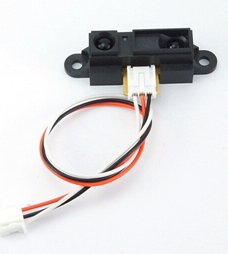
\includegraphics[width=3.861cm,height=4.3cm]{text05-img/text05-img030.png} \newline
図 \stepcounter{qwerty}{\theqwerty}: 距離センサー}
\end{minipage}\  }
\end{minipage}  \begin{minipage}{7.601cm}
\begin{minipage}{7.601cm}
{\upshape
 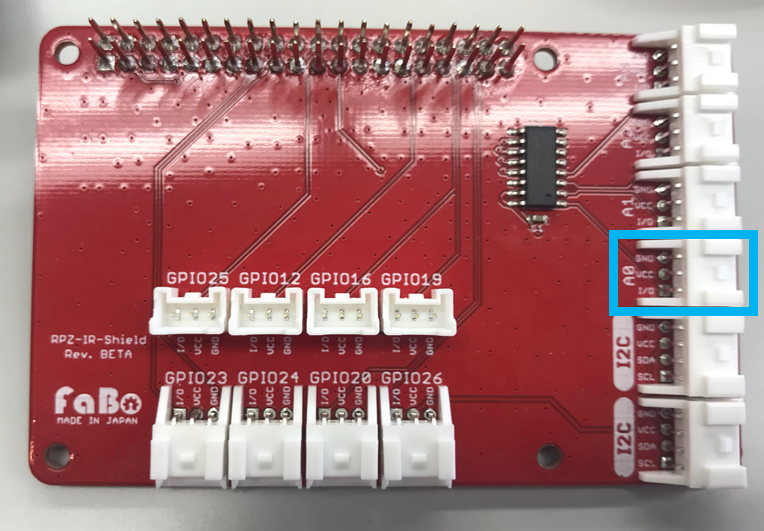
\includegraphics[width=7.601cm,height=4.549cm]{text05-img/text05-img029.png} \newline
図 \stepcounter{qwerty}{\theqwerty}: A0}
\end{minipage}
\end{minipage}
\par}

データはspigetを使って受け取ることができます。値は0〜1023になります。これでは距離がわからないので、受け取った値を距離に変換する必要があります。変換するための式は\pageref{bkm:RefHeadingToc5917367650265}ページに書いてあります。今回は入力はdataという変数にしているので、式のxをdataにします。\textcolor{black}{kyori
=
-1*(data*5000/1023)/36+845/9で入力を距離に変換し、kyori変数に代入しています。単位はcmです。}

%\begin{figure}
\centering
\begin{minipage}{17.006cm}
{\ttfamily\bfseries
\#include {\textquotedbl}hsp3dish.as{\textquotedbl}}

{\ttfamily\bfseries
\#include {\textquotedbl}rpz-gpio.as{\textquotedbl}}


\bigskip

{\ttfamily\bfseries
spiopen 0}


\bigskip

{\ttfamily\bfseries
*main}


\bigskip

{\ttfamily\bfseries
\ \ data =
spiget(0,0)\ \ \textcolor[rgb]{0.0,0.0,0.6}{;SPIを使ってデータを受け取る}}

{\ttfamily\bfseries
\ \ \textcolor{black}{kyori = -1*(data*5000/1023)/36+845/9}\textcolor[rgb]{0.0,0.0,0.6}{ ;
dataを距離に変換しています}}

{\ttfamily\bfseries
\ \ res = {\textquotedbl}距離 : {\textquotedbl}+kyori}


\bigskip

{\ttfamily\bfseries
\ \ redraw 0}

{\ttfamily\bfseries
\ \ font {\textquotedbl}{\textquotedbl},20}

{\ttfamily\bfseries
\ \ pos 30,30}

{\ttfamily\bfseries
\ \ mes res}

{\ttfamily\bfseries
\ \ redraw 1}


\bigskip

{\ttfamily\bfseries
\ \ wait 100}

{\ttfamily\bfseries
\ \ goto *main}


\bigskip

{\ttfamily\bfseries
spiclose 0}

{\mdseries
リスト \stepcounter{List}{\theList}: kyori.hsp}
\end{minipage}
%\end{figure}
{\bfseries
\textcolor{black}{問題 5-\stepcounter{qwertya}{\theqwertya}}}

\textcolor{black}{距離センサー(番号は書いてありません。\pageref{bkm:RefHeadingToc5917367650265}ページを参考にしてください)をA0につなげ}\textcolor{black}{てkyori.hspを実行してみましょう。距離はだいたい5〜80cmです。\newline
}

\clearpage\subsection{ゆうきELディスプレイを使ってみよう}
{\mdseries
ゆうきELディスプレイをHSPで使ってみましょう。I2CにゆうきELディスプレイ(\#214)をつないでみましょう。HSPスクリプトエディタで/home/pi/ome/05/oled.hspを開いて実行してください。}

{\centering
\begin{minipage}{4.283cm}
\begin{minipage}{4.283cm}
{\upshape
 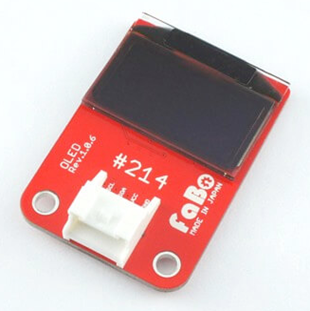
\includegraphics[width=4.283cm,height=4.135cm]{text05-img/text05-img031.png} \newline
図 \stepcounter{qwerty}{\theqwerty}: ゆうきELディスプレイ}
\end{minipage}
\end{minipage}   \begin{minipage}{6.959cm}
\begin{minipage}{6.959cm}
{\upshape
 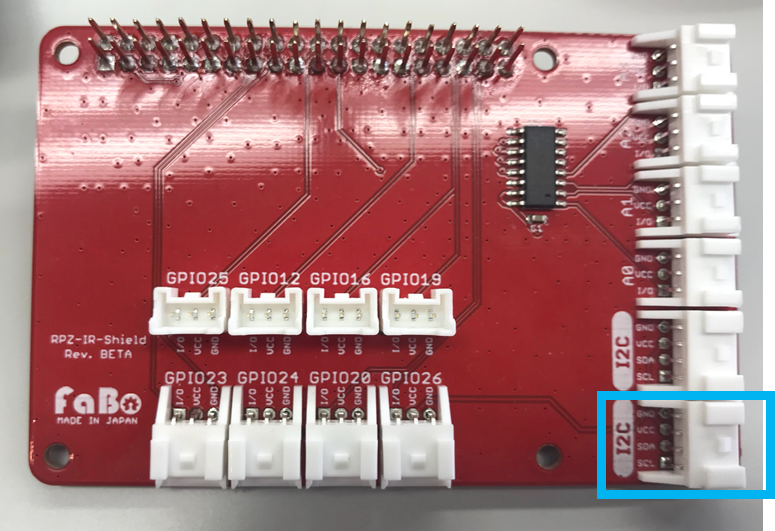
\includegraphics[width=6.959cm,height=4.755cm]{text05-img/text05-img032.png} \newline
図 \stepcounter{qwerty}{\theqwerty}: I2C}
\end{minipage}
\end{minipage}
\par}

ゆうきELディスプレイに文字を表示するにはoled命令を使います。\newline
\texttt{\textbf{oled ``表示したい文字''}}\newline
と使います。日本語は打つことができません。英語か記号を表示することができます。,(カンマ)を使って、改行することができます。

%\begin{figure}
\centering
\begin{minipage}{17.006cm}
{\ttfamily\bfseries
\#include {\textquotedbl}hsp3dish.as{\textquotedbl}}

{\ttfamily\bfseries
\#include {\textquotedbl}rpz-gpio.as{\textquotedbl}}


\bigskip

{\ttfamily\bfseries
redraw 0}

{\ttfamily\bfseries
font {\textquotedbl}{\textquotedbl},20}

{\ttfamily\bfseries
pos 20,20}

{\ttfamily\bfseries
mes
{\textquotedbl}有機ELディスプレイを見てね{\textbackslash}nカンマ(,)で改行するよ{\textquotedbl}}

{\ttfamily\bfseries
redraw 1}


\bigskip

{\ttfamily\bfseries
oled {\textquotedbl}Good Morning,Good Bye,Good Afternoon{\textquotedbl}\newline
\textcolor[rgb]{0.0,0.0,0.6}{;ELディスプレイに}}

{\ttfamily\bfseries\color[rgb]{0.0,0.0,0.6}
;Good Morning}

{\ttfamily\bfseries\color[rgb]{0.0,0.0,0.6}
;Good Bye\newline
;Good Afternoon\newline
;と表示します。}


\bigskip

{\ttfamily\bfseries
wait 100}

{\mdseries
リスト \stepcounter{List}{\theList}: oled.hsp}
\end{minipage}
%\end{figure}

\bigskip

{\bfseries
問題 5-\stepcounter{qwertya}{\theqwertya}}

自分の名前(アルファベット)をゆうきELディスプレイ(\#214)に表示してみましょう


\bigskip

{\bfseries
問題 5-\stepcounter{qwertya}{\theqwertya}}

自分の名前の下に、隣の人の名前(アルファベット)をゆうきELディスプレイ(\#214)に表示してみましょう。


\bigskip

\subsection{ボリュームを使って画像を動かしてみよう}
A0にボリューム(\#104)をつなげてみましょう。HSPスクリプトエディタで/home/pi/ome/05/angle.hspを開いて実行してください。

画像を使うためにはcelload命令を使います。

%\begin{figure}
\centering
\begin{minipage}{17.006cm}
{\ttfamily\bfseries
\#include {\textquotedbl}hsp3dish.as{\textquotedbl}}

{\ttfamily\bfseries
\#include {\textquotedbl}rpz-gpio.as{\textquotedbl}}


\bigskip

{\ttfamily\bfseries
celload({\textquotedbl}hyou.png{\textquotedbl}),2\ \ \textcolor[rgb]{0.0,0.0,0.6}{;hyou.pngを読み込む}}

{\ttfamily\bfseries
p = 50}


\bigskip

{\ttfamily\bfseries
spiopen 0}


\bigskip

{\ttfamily\bfseries
*main}

{\ttfamily\bfseries
\ \ data = spiget(0,0)\ \ \textcolor[rgb]{0.0,0.0,0.6}{;データを受け取る}}

{\ttfamily\bfseries
\ \ p = rasp\_map(data, 0, 1023, 0,
440)\ \ \ \ \textcolor[rgb]{0.0,0.0,0.6}{;値を0〜440に変換する}}


\bigskip

{\ttfamily\bfseries
\ \ redraw 0}

{\ttfamily\bfseries
\ \ pos 20,20}

{\ttfamily\bfseries
\ \ mes data}

{\ttfamily\bfseries
\ \ mes p}

{\ttfamily\bfseries
\ \ pos 0,0\ \ \textcolor[rgb]{0.0,0.0,0.6}{;画像の位置を決める}}

{\ttfamily\bfseries
\ \ celput 2\ \ \textcolor[rgb]{0.0,0.0,0.6}{;画像2を置く}}

{\ttfamily\bfseries
\ \ redraw 1}


\bigskip

{\ttfamily\bfseries
\ \ wait 10\ \ }

{\ttfamily\bfseries
\ \ goto *main}


\bigskip

{\ttfamily\bfseries
spiclose 0}

{\mdseries
リスト \stepcounter{List}{\theList}: angle.hsp}
\end{minipage}
%\end{figure}
{\bfseries
celload (``画像の名前''),画像の番号}

で画像を読み込むことができます。読み込んだ画像は\textbf{celput
画像の番号}で表示することができます。画像や文字の位置は\texttt{\textbf{pos}}命令を使って決めることができます。pos命令で画像の位置がどう変わるのか、
図 24:
画面と位置のかんけいを見てみましょう。


\bigskip


\bigskip

\clearpage\begin{minipage}{16.282cm}
{\upshape
 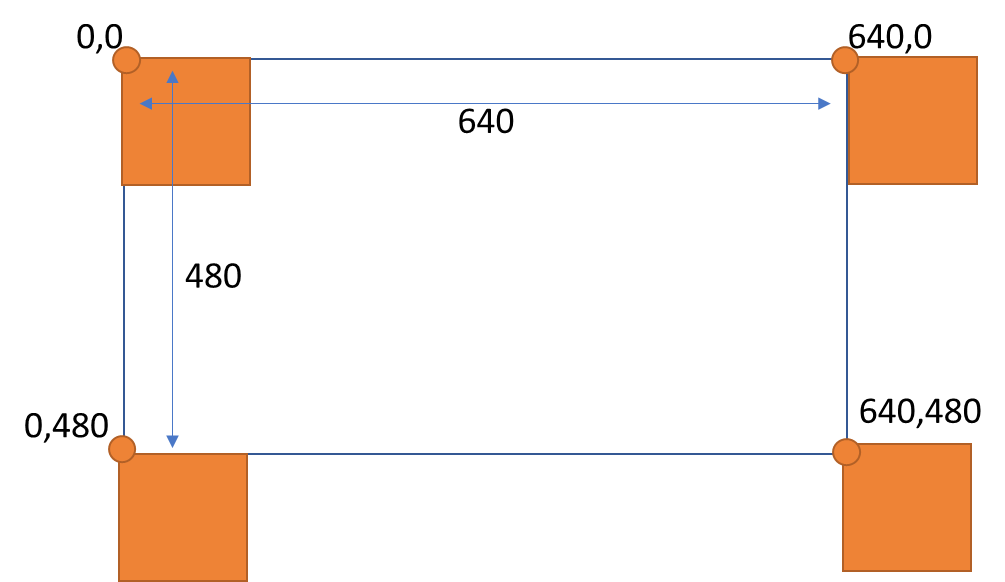
\includegraphics[width=17.006cm,height=9.848cm]{text05-img/text05-img033.png} \newline
図 {\refstepcounter{qwerty}\theqwerty\label{seq:ref23}}:
画面と位置のかんけい}
\end{minipage}


\bigskip

みなさんが使っているHSPでは画面の横のサイズは640、縦のサイズは480で表示されています。青い四角が画面、オレンジの四角が画像だと思ってください。画像や文字の位置は\texttt{\textbf{pos
横の位置,縦の位置}}を使って決めます。横の位置は一番左からどれくらい離れているか、縦の位置は一番上からどれくらい離れているかで決まります。例えば左上は0,0と書くことができます。右下は640,480と書くことができます。一番右上に画像を表示したいとき、640,0と書いてしまうと画像がディスプレイからはみ出てしまいます。pos命令では画像の左上の点をどこに置くか指定しているからです。画像をディスプレイの中にいれたいときは、画像のサイズ分だけposで指定する位置を左にずらさないといけません。


\bigskip

{\bfseries
問題 5-\stepcounter{qwertya}{\theqwertya}}

ボリューム(\#104)をA0につなげて/home/pi/ome/05/block3\_angle.hspを実行してみましょう。ボリューム(\#104)を使ってブロック崩しを遊ぶことができます。


\bigskip

{\bfseries
問題 5-\stepcounter{qwertya}{\theqwertya}}

angle.hspの \texttt{\textbf{pos 0,0}}\texttt{
}の数字を変えて、右上に画像を表示しましょう。\newline
(だいたいで良いです)


\bigskip

{\bfseries
問題 5-\stepcounter{qwertya}{\theqwertya}}

angle.hspの \texttt{\textbf{pos 0,0}}\texttt{
}の数字を変えて、真ん中に画像を表示しましょう。\newline
(だいたいで良いです)


\bigskip

{\bfseries
問題 5-\stepcounter{qwertya}{\theqwertya}}

angle.hspの \texttt{\textbf{pos 0,0}}\texttt{
}の数字を変えて、左下に画像を表示しましょう。\newline
(だいたいで良いです)


\bigskip

{\bfseries
問題 5-\stepcounter{qwertya}{\theqwertya}}

angle.hspの \texttt{\textbf{pos 0,0}}\texttt{
}の数字を変えて、右下に画像を表示しましょう。\newline
(だいたいで良いです)


\bigskip

{\bfseries
問題 5-{\refstepcounter{qwertya}\theqwertya\label{seq:ref24}}}

ボリュームを使って画像を横に動かしてみましょう。\newline
angle.hspの\texttt{\textbf{pos 0,0}}を\texttt{\textbf{pos
p,0}}に変えて実行してください。


\bigskip

{\bfseries
チャレンジ問題 5-\stepcounter{qwertyb}{\theqwertyb}}

??~\ref{seq:ref24}では、ボリュームの値を大きくすると、ヒョウが右に動きます。ボリュームの入力は\textbf{data
= spiget(0,0)}で受け取り、\textbf{p = rasp\_map(data, 0, 1023, 0,
440)}で値を0〜440に変換します。ボリュームの値で画像を右に動かすには、変数を使います。pには0〜440の値が入るため、pos命令で横をpにすればボリュームの値で右に動かすことができます。

時間があったら挑戦してみましょう。\newline
ボリュームの値を大きくしていくと、画像が右から左に動くようにプログラムを変えましょう。


\bigskip

{\bfseries
チャレンジ問題 5-\stepcounter{qwertyb}{\theqwertyb}}

時間があったら挑戦してみましょう。\newline
ボリュームの値で画像が縦に動くようにプログラムを変えましょう。\newline


\clearpage\subsection{LEDの明るさを変える}
{\mdseries
HSPスクリプトエディタで/home/pi/ome/05/pwm.hspを開いて実行してください。}

[Warning: Draw object
ignored]緑色のLEDは明るさが弱く、白色のLEDは明るさが強くなっています。LEDを光らせるためには1、消すためには0を使います。1秒や2秒ごとに1と0を切りかえると、LEDが点いたり消えたりするのが人間でもわかります。けれどプログラムがもっと高速に1と0を切りかえると、人間にはわからずLEDがずっと光っているように見えます。それを利用して、一定時間の間のLEDの消灯時間の比率で明るさに強弱をつけることができます。

%\begin{figure}
\centering
\begin{minipage}{17.006cm}
{\ttfamily\bfseries
\#include {\textquotedbl}hsp3dish.as{\textquotedbl}}

\begin{minipage}{17.006cm}
{\ttfamily\bfseries
repeat 200}

{\ttfamily\bfseries
if cnt {\textless} 10 : gpio 17,1 : else : gpio 17,0}

{\ttfamily\bfseries
if cnt {\textless} 50 : gpio 18,1 : else : gpio 18,0}

{\ttfamily\bfseries
if cnt {\textless} 100 : gpio 22,1 : else : gpio 22,0}

{\ttfamily\bfseries
loop}
\end{minipage}{\ttfamily\bfseries
\#include {\textquotedbl}rpz-gpio.as{\textquotedbl}}


\bigskip

{\ttfamily\bfseries
redraw 0}

{\ttfamily\bfseries
redraw 1}


\bigskip

{\ttfamily\bfseries
repeat}

{\ttfamily\bfseries
gpio 27,1}

{\ttfamily\bfseries
await 1}

{\ttfamily\bfseries
loop}


\bigskip

{\ttfamily\bfseries
gpio 17,0}

{\ttfamily\bfseries
gpio 18,0}

{\ttfamily\bfseries
gpio 22,0}

{\ttfamily\bfseries
gpio 27,0}

{\ttfamily\bfseries
stop}

{\mdseries
リスト \stepcounter{List}{\theList}: pwm.hsp}
\end{minipage}
%\end{figure}
\begin{minipage}{16.854cm}
%\newline

\begin{minipage}{14.63cm}
{\upshape
 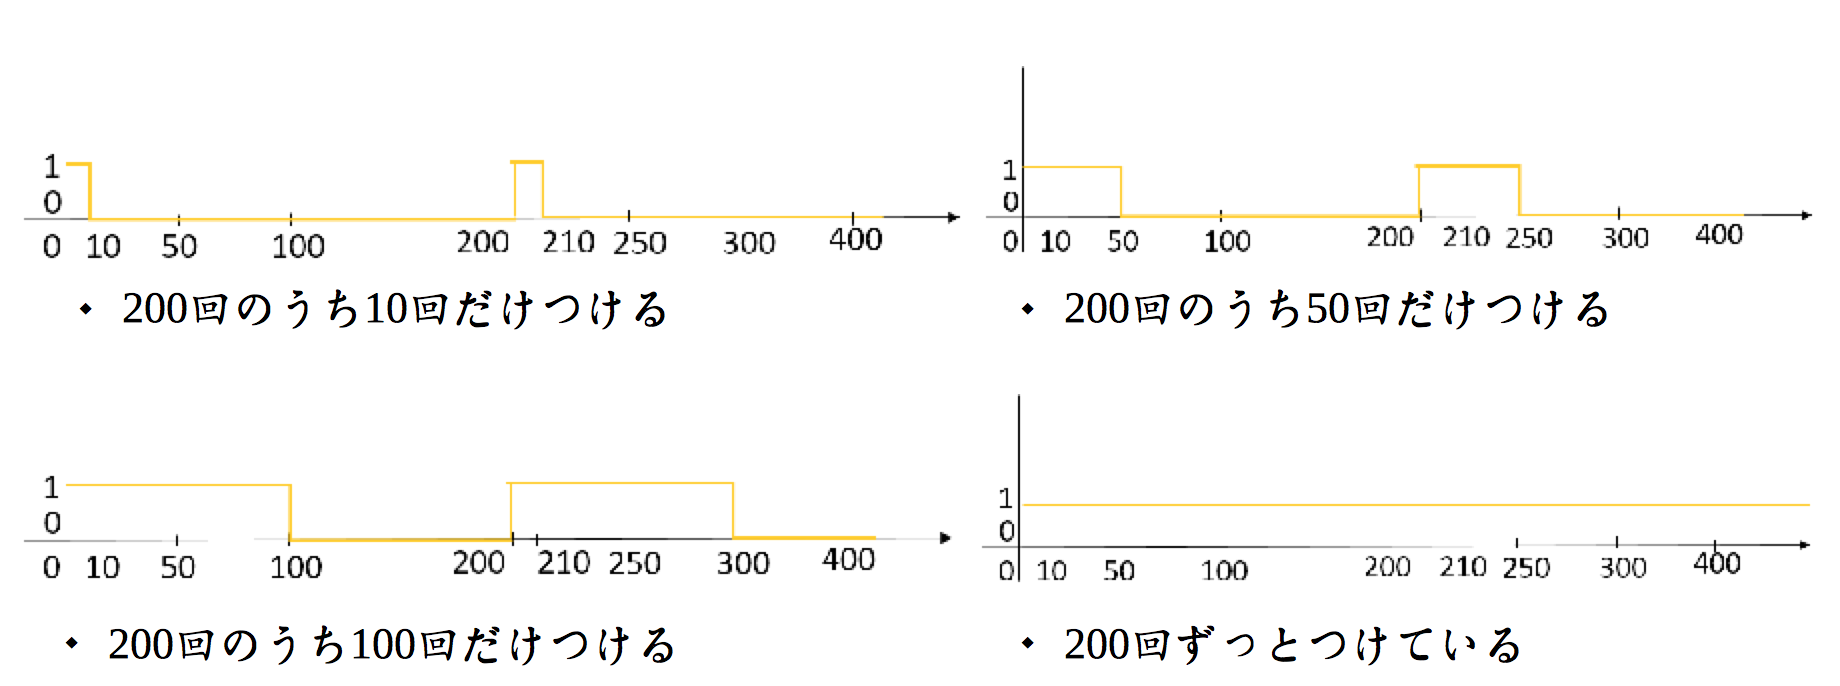
\includegraphics[width=14.63cm,height=5.454cm]{text05-img/text05-img034.png} \newline
図 \stepcounter{qwerty}{\theqwerty}: PWM}
\end{minipage}\end{minipage}

青線で囲まれた部分を見てみましょう。repeat
200で3つのif文を200回繰り返しています。GPIO17はカウントが10より小さいときだけLEDをつけます。200回のうち10回しかつけていないので、光が弱くなっています。GPIO22はカウントが100回より小さいときLEDをつけます。200のうち100回もLEDをつけているので、LEDはGPIO17より強くなっています。

\clearpage\section{赤外線}
\subsection[赤外線ってなんだろう?]{\rmfamily
赤外線ってなんだろう?}
\begin{minipage}{14.923cm}
{\upshape
 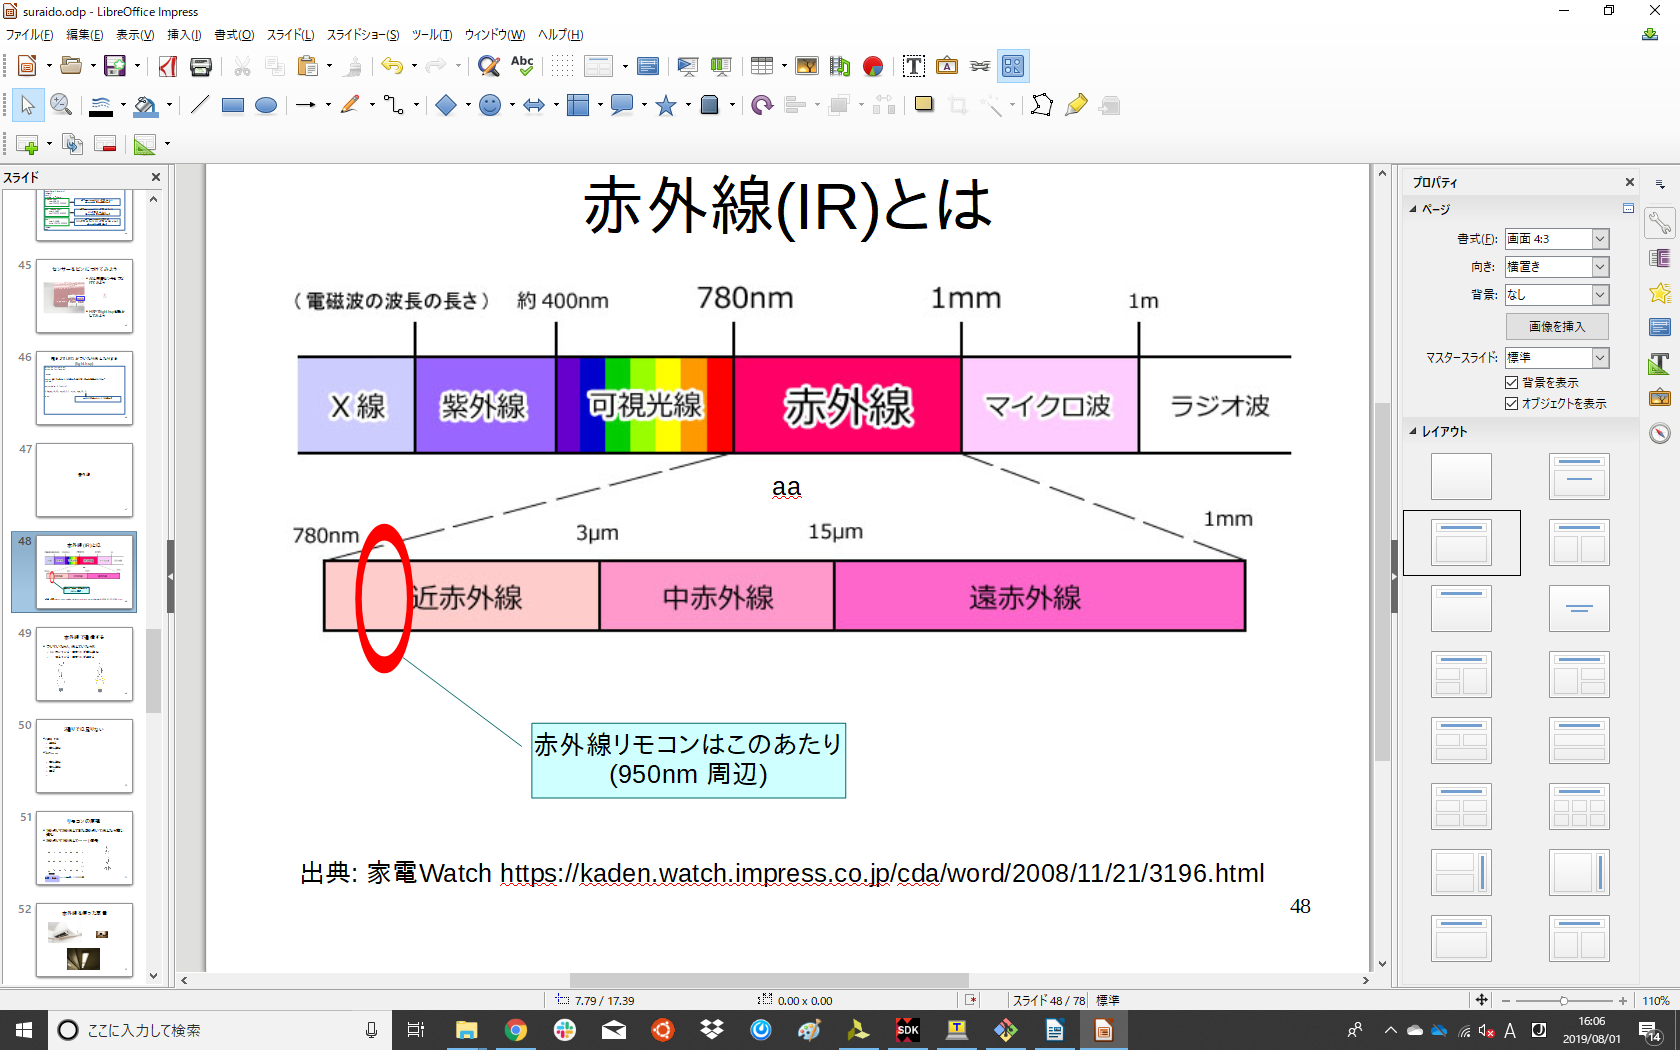
\includegraphics[width=14.923cm,height=8.98cm]{text05-img/text05-img035.png} \newline
図 \stepcounter{qwerty}{\theqwerty}: 電磁波。出典: 家電 Watch
https://kaden.watch.impress.co.jp/cda/word/2008/11/21/3196.html}
\end{minipage}

 物質や生物はそれぞれ電磁波を発しています。X線、紫外線、光、マイクロ波などは電磁波の一種です。電磁波は波であり、どれだけ振動しているかで種類をわけることができます。わたしたちは可視光線と呼ばれる光が目に入ることで、色などを目で感知することができます。マイクロ波は電子レンジに使われています。マイクロ波によって物質を振動させることで、物質の温度をあげています。

 赤外線は人の目には見えません。けれどすべての物体が赤外線を発しています。特に温度の高いものは赤外線を強く発しています。Raspberry
Piは発熱しながら動いています。Raspberry
Piに触れなくても、手を近づけるだけで熱を感じるのは、赤外線がRaspberry
Piから発せられていて、その赤外線を手で感知しているからです。

 赤外線を使って信号を送ったり、受け取ったりすることもできます。例えば赤外線が送られているときは電気をつける、赤外線が送られていないときは電気を消すことができます。しかし送られているかどうかだけではつける、消すしかできません。ロボットのように歩く、止まる、右に曲がる、左に曲がるなど多くの動きを制御したいときは、信号を組み合わせて送ります。

  図 27:
赤外線で信号を送る方法を見てみましょう。電球が点いているときは赤外線を送り、電球が消えていないときは赤外線を送っていないという意味です。例えば1/1000000秒の間隔で赤外線を送ります。つけたり消したりを組み合わせて、いろいろなパターンを作ることができます。そのパターンによって制御を決めています。送る、送らない、送らない、送らない、送る、送る、送らないと信号が来たときは''歩く{}''と制御します。

%\begin{figure}
\centering
\begin{minipage}{12.367cm}
{\upshape
 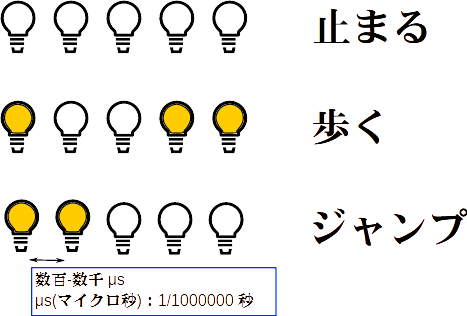
\includegraphics[width=12.367cm,height=8.373cm]{text05-img/text05-img036.png} \newline
図 {\refstepcounter{qwerty}\theqwerty\label{seq:ref26}}:
赤外線で信号を送る方法}
\end{minipage}
%\end{figure}
\subsection[赤外線をつかった家電]{\rmfamily
赤外線をつかった家電}
 もっと身近なもので考えてみましょう。赤外線を使った家電はなにがあるでしょうか?

\begin{center}
\tablefirsthead{}
\tablehead{}
\tabletail{}
\tablelasttail{}
\begin{supertabular}{|l|l|l|}
\hline
\multicolumn{1}{|c|}{
\begin{minipage}{4.165cm}
\upshape  
\includegraphics[width=4.165cm,height=4.165cm]{text05-img/text05-img037.png} \newline
図 \stepcounter{qwerty}{\theqwerty}: テレビ\end{minipage}
} & \multicolumn{1}{c|}{
\begin{minipage}{4.576cm}
\upshape  
\includegraphics[width=4.576cm,height=4.576cm]{text05-img/text05-img038.png} \newline
図 \stepcounter{qwerty}{\theqwerty}: エアコン\end{minipage}
} & 
\begin{minipage}{4.387cm}
\upshape  
\includegraphics[width=4.387cm,height=4.387cm]{text05-img/text05-img039.png} \newline
図 \stepcounter{qwerty}{\theqwerty}: せんぷう機\end{minipage}
\\\hline
\end{supertabular}
\end{center}

\bigskip

 テレビ、エアコン、せんぷう機などはリモコンを使って動作を制御しています。ボタンを押せば電源が点いたり、風量や音量を調節できます。これは赤外線を使って家電を制御しています。電源を入れるときはリモコンから電源を入れるための赤外線信号が送られます。家電はそれを受け取り、信号で決められた動作をします。

\clearpage\subsection[Raspberry Piをリモコンにしよう]{\rmfamily Raspberry
Piをリモコンにしよう}
 Raspberry
Piにも赤外線を送ったり、受け取ることができるセンサーがついています。これを使って何ができるでしょうか?Raspberry
Piをリモコンにして家電を制御することができます。

\begin{itemize}
\item
リモコンをひとつにまとめることができる
\item
外出先から家電を操作することができる
\item
音声を使って家電を操作することができる
\end{itemize}
 Raspberry
Piをリモコンにするためには、リモコンの真似をすることが必要です。リモコンから赤外線の信号をセンサーボードの赤外線受信ユニットで受け取ります。コマンドを使って信号をテキストに変換します。変換された信号を赤外線センサーから家電に送信することで、リモコンと同じ信号を家電に送ることができます。


\bigskip



%\begin{figure}
\centering
\begin{minipage}{17.006cm}
{\upshape
 
\includegraphics[width=17.006cm,height=9.368cm]{text05-img/text05-img040.png} \newline
図 \stepcounter{qwerty}{\theqwerty}: Raspberry
Piをリモコンにする手順}
\begin{minipage}{3.731cm}
信号をテキストにする
\end{minipage}\end{minipage}
%\end{figure}

\bigskip

\clearpage{\bfseries
問題
5-\stepcounter{qwertya}{\theqwertya} リモコンの信号をコピーしてみよう}

ターミナルを開いて、コマンドを入力しましょう。

\begin{enumerate}
\item
リモコンの信号を受け取り、ファイルに記録します。

\begin{enumerate}
\item /home/pi/ome/05に移動します。

\texttt{\textbf{cd /home/pi/ome/05}}
\item
違う信号を受け取らないように、赤外線受信を止めます。\newline
\texttt{\textbf{sudo service lircd stop}}
\item
赤外線を受信し、onoff.txtに記録します。コマンドを実行してから、赤外線受信ユニットに向かって、リモコンのボタンを押しましょう。記録が終わったらCtrl+c(Ctrlキーを押しながらcを押す)で終了します。\newline
\texttt{\textbf{mode2 -d /dev/lirc0 {\textbar} tee onoff.txt}}
\item
記録した信号を、送信用に変換します。\newline
\texttt{\textbf{convert\_pattern onoff.txt {\textgreater} onoff.pattern}}
\item
設定ファイルを作ります。\texttt{\textbf{/home/pi/ome/05/template.lircd.conf}}を元に作ります。まずはこのテンプレートを\textbf{05.lircd.conf}という名前でコピーします。そのあと、leafpadで開きましょう。\newline
\texttt{\textbf{cp template.lircd.conf 05.lircd.conf\newline
leafpad 05.lircd.conf}}\newline
リスト 8:
template.lircd.confの赤字の部分を書き換えます。\newline
		\begin{enumerate}
			\item
リモコンの名前を決めます。使う家電の名前(fan,
robot, TV...)にしましょう。\newline
			\item
信号の名前を決めます。動作(digital\_onoff,walk...)の名前にしましょう。\newline
			\item
``ここに信号をペーストする''と書いてある行を消します。onoff.patternに書かれた信号をコピーして貼り付けます。leafpadを使ってonoff.patternを表示しましょう。
		\end{enumerate}
\texttt{\textbf{leafpad onoff.pattern}}\newline
onoff.patternに書かれた信号は、たとえば「1207 588
447 838 447 823 475 812
1218」のような文字列です。ただし、ここに書くことができる数字の数は255以下にしないといけないことに注意してください。書き換えた後に数を数えて、255個以下であることを確認しましょう。\newline
書き換えたら、保存しましょう
(名前が05.lircd.confになっていることを確認しましょう)。
\end{enumerate}
\end{enumerate}


%\begin{figure}
\centering
\begin{minipage}{17.006cm}
[Warning: Draw object ignored][Warning: Draw object ignored][Warning: Draw object ignored]begin remote


\bigskip

\ \ \ \ \ \ \ \ name \textcolor[rgb]{1.0,0.2,0.2}{fan}

\ \ \ \ \ \ \ \ flags RAW\_CODES

\ \ \ \ \ \ \ \ eps 30

\ \ \ \ \ \ \ \ aeps 100


\bigskip

\ \ \ \ \ \ \ \ gap 200000

\ \ \ \ \ \ \ \ toggle\_bit\_mask 0x0


\bigskip

\ \ \ \ \ \ \ \ begin raw\_codes

\ \ \ \ \ \ \ \ name \textcolor[rgb]{1.0,0.2,0.2}{onoff}

\textcolor[rgb]{0.5019608,0.5019608,0.5019608}{\ \ }\textcolor[rgb]{1.0,0.2,0.2}{ここに信号をペーストする}

\ \ \ \ \ \ \ \ end raw\_codes


\bigskip

end remote

{\mdseries
リスト {\refstepcounter{List}\theList\label{seq:refList8}}: template.lircd.conf}
\end{minipage}
%\end{figure}
%\setcounter{saveenum}{\value{enumi}}
\begin{enumerate}
%\setcounter{enumi}{\value{saveenum}}
\item \clearpage
ファイルに記録された信号を、赤外線LEDから送信する。

%\setcounter{saveenum}{\value{enumii}}
\begin{enumerate}
%\setcounter{enumii}{\value{saveenum}}
\item 設定ファイルをコピーします。\newline
sudo cp 05.lircd.conf /etc/lirc/lircd.conf.d/
\item
設定ファイルを再読み込みします。\newline
sudo service lircd restart
\item
赤外線を送ります。fanは設定ファイルに書いたリモコンの名前、onoffは設定ファイルに書いた信号の名前に変えましょう。\newline
irsend SEND\_ONCE \textcolor[rgb]{1.0,0.2,0.2}{fan} \textcolor[rgb]{1.0,0.2,0.2}{onoff}
\end{enumerate}
\end{enumerate}

\bigskip

\subsection[]{[Warning: Draw object ignored]}
%\begin{figure}
\centering
\begin{minipage}{17.006cm}
{\upshape
 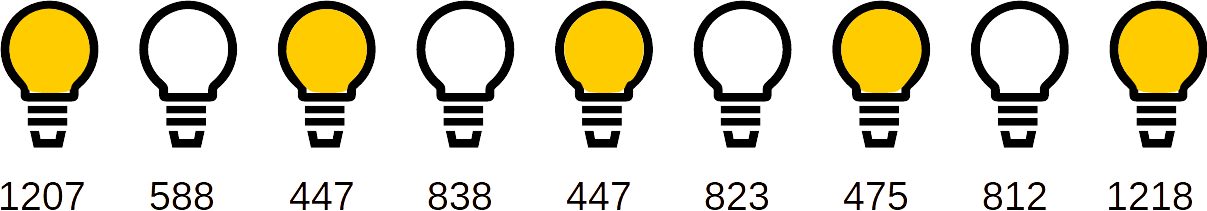
\includegraphics[width=17.006cm,height=2.972cm]{text05-img/text05-img041.png} \newline
図 \stepcounter{qwerty}{\theqwerty}:
信号のイメージ 数字にある時間で点灯/消灯が切り替わる}
\end{minipage}
%\end{figure}
\clearpage\subsection[\ HSPを使って赤外線を出力するプログラムを作ってみよう]{\ HSPを使って赤外線を出力するプログラムを作ってみよう}
HSPスクリプトエディタで/home/pi/ome/05/ir.hspを開いてみましょう。\newline
HSPではexec命令を使ってターミナルで使うコマンドを実行することができます。

{\ttfamily\bfseries
exec {\textquotedbl}irsend SEND\_ONCE fan onoff{\textquotedbl}}

exec
``コマンド''と使います。コマンドは先ほどターミナルで実行したirsend
SEND\_ONCE \textcolor[rgb]{1.0,0.2,0.2}{fan}
\textcolor[rgb]{1.0,0.2,0.2}{onoff}\textcolor{black}{です。}\textcolor[rgb]{1.0,0.2,0.2}{fan}\textcolor{black}{はリモコンの名前、}\textcolor[rgb]{1.0,0.2,0.2}{onoff}\textcolor{black}{は信号の名前でしたね。}\textcolor[rgb]{1.0,0.2,0.2}{fan}\textcolor{black}{と}\textcolor[rgb]{1.0,0.2,0.2}{onoff}\textcolor{black}{は自分で設定ファイルに書いた名前に変えましょう。}



%\begin{figure}
\centering
\begin{minipage}{17.006cm}
{\ttfamily\bfseries
\#include {\textquotedbl}hsp3dish.as{\textquotedbl}}

{\ttfamily\bfseries
\#include {\textquotedbl}rpz-gpio.as{\textquotedbl}}


\bigskip

{\ttfamily\bfseries
BUTTON\_PIN = 24}

{\ttfamily\bfseries
prev = 0}

{\ttfamily\bfseries
status=0}


\bigskip

{\ttfamily\bfseries
*main}

{\ttfamily\bfseries
\ \ \ \ \ \ \ \ gpmes
{\textquotedbl}ボタンPUSHで赤外線照射!{\textquotedbl}}

{\ttfamily\bfseries
\ \ \ \ \ \ \ \ goto *edge}


\bigskip

{\ttfamily\bfseries
*edge}

{\ttfamily\bfseries
\ \ \ \ \ \ \ \ current = gpioin(BUTTON\_PIN)}

{\ttfamily\bfseries
\ \ \ \ \ \ \ \ if (prev=0) \& (current=1)
\{\ \ \ \ \ \ \textcolor[rgb]{0.2,0.2,1.0}{;ボタンが押されたら}}

{\ttfamily\bfseries
\ \ \ \ \ \ \ \ \ \ \ \ \ \ \ \ exec {\textquotedbl}irsend SEND\_ONCE \textcolor[rgb]{1.0,0.2,0.2}{fan}
\textcolor[rgb]{1.0,0.2,0.2}{onoff}{\textquotedbl}\ \ \textcolor[rgb]{0.2,0.2,1.0}{;irsendコマンドを実行する}}

{\ttfamily\bfseries
\ \ \ \ \ \ \ \ \}}

{\ttfamily\bfseries
\ \ \ \ \ \ \ \ prev = current}

{\ttfamily\bfseries
\ \ \ \ \ \ \ \ update 1}

{\ttfamily\bfseries
\ \ \ \ \ \ \ \ goto *edge}


\bigskip

{\mdseries
リスト \stepcounter{List}{\theList}: ir.hsp}
\end{minipage}
%\end{figure}
{\bfseries
問題 5-\stepcounter{qwertya}{\theqwertya}}

\begin{enumerate}
\item
ボタンをGPIO24につなげ、自分でコピーした赤外線を出力してみましょう。\newline
\textcolor[rgb]{1.0,0.2,0.2}{fan}\textcolor{black}{と}\textcolor[rgb]{1.0,0.2,0.2}{onoff}\textcolor{black}{は自分で設定ファイルに書いた名前に変えましょう。\newline
}
\end{enumerate}
\subsection{赤外線送受信のまとめ}
\begin{enumerate}
\item sudo service lircd stop
\item mode2 -d /dev/lirc0{\textbar} tee ファイル名1.txt
\item convert\_pattern ファイル名1.txt {\textgreater}
ファイル名2.pattern
\item
template.lircd.confを書きかえてファイル名3.lircd.confを作成
\item sudo cp ファイル名3.lircd.conf /etc/lirc/lircd.conf.d/
\item sudo service lircd restart
\item irsend SEND\_ONCE {\textless}リモコンの名前{\textgreater}
{\textless}信号の名前{\textgreater}
\end{enumerate}
\subsection{おまけ:信号を2つ以上登録する}
複数の動作を制御したい場合は、動作ごとに信号を登録する必要があります。template.lircd.confの中の``begin
raw\_codes'' と ``end raw\_codes''の間にname
{\textless}名前{\textgreater}と信号を並べることで複数の信号を登録することができます。ただし、信号をあらわす数字の数は255個以下でないといけないと書きましたが、これはファイルひとつにある信号を全て合わせたものであることに注意してください。この場合、onoffに記述される数字の数と、powerに記述される数字の数の和が255以下でなければなりません。

[Warning: Draw object ignored]

%\begin{figure}
\centering
\begin{minipage}{17.006cm}
begin remote

\ \ name fan

\ \ flags RAW\_CODES

\ \ eps 30

\ \ aeps 100


\bigskip

\ \ gap 200000

\ \ toggle\_bit\_mask 0x0


\bigskip

\ \ begin raw\_codes


\bigskip

\ \ \ \ \ \ name onoff

\ \ \ \ \ \ 1207 588 447 838 447 823 475 812 1218{\dots}


\bigskip

\ \ \ \ \ \ \textcolor[rgb]{1.0,0.2,0.2}{name power}

{\color[rgb]{1.0,0.2,0.2}
\ \ \ \ \ \ 1364 363 752 743 372 836 164 614 ...}


\bigskip

\ \ end raw\_codes


\bigskip

end remote


\bigskip


\bigskip


\bigskip


\bigskip

{\mdseries
リスト \stepcounter{List}{\theList}:
2つの信号を登録するときのtemplate.lircd.comf}
\end{minipage}
%\end{figure}
\subsection{宿題}
自分の家にある家電をRaspberry
Piで制御してみましょう。エアコン、扇風機、テレビなど赤外線を使って操作する家電を選びましょう。

\clearpage\section{ふろく:センサー紹介}
\label{bkm:RefHeadingToc37441454936466}\subsection[デジタル出力そうち]{\rmfamily
デジタル出力そうち}
\subsubsection[\ LED]{\ LED}
\label{bkm:RefHeadingToc25509508239293}
\bigskip

\begin{flushleft}
\tablefirsthead{}
\tablehead{}
\tabletail{}
\tablelasttail{}
\begin{supertabular}{|m{4.2450004cm}|m{6.6260004cm}|}
\hline
\centering 名称 &
\centering\arraybslash LED(えるいーでぃー)\\\hline
\centering 接続箇所 &
\centering\arraybslash デジタルコネクタ (3pin)\\\hline
\centering 機能概要 &
\centering\arraybslash LEDを点灯させる\\\hline
\end{supertabular}
\end{flushleft}

\bigskip

\begin{flushleft}
\tablefirsthead{}
\tablehead{}
\tabletail{}
\tablelasttail{}
\begin{supertabular}{|m{3.769cm}|m{12.844cm}|}
\hline
\centering サンプルコードの場所 &
\centering\arraybslash ome/05/digout.hsp\\\hline
\centering raspiへの入力 &
\centering\arraybslash なし\\\hline
\centering raspiへの入力方法 &
\centering\arraybslash なし\\\hline
\centering raspiからの出力 &
\centering\arraybslash
値が1の時点灯、値が0の時消灯\\\hline
\centering raspiからの出力方法 &
\centering\arraybslash gpio GPIO番号, パラメータ\\\hline
\end{supertabular}
\end{flushleft}

\bigskip


\bigskip

\begin{flushleft}
\tablefirsthead{}
\tablehead{}
\tabletail{}
\tablelasttail{}
\begin{supertabular}{|m{3.769cm}|m{12.844cm}|}
\hline
\centering 使い道 &
\centering\arraybslash 照明、信号機、車のライト\\\hline
\centering 注意事項 &
\centering\arraybslash なし\\\hline
\centering 補足 &
\centering\arraybslash
プラスとマイナスの電流がLEDチップ内で衝突するエネルギーを利用して発光します。LEDの光の色はLEDチップに含まれている半導体の種類で決まっています\\\hline
\end{supertabular}
\end{flushleft}

\bigskip

\begin{flushleft}
\tablefirsthead{}
\tablehead{}
\tabletail{}
\tablelasttail{}
\begin{supertabular}{|m{1.0699999cm}|m{6.4680004cm}|m{1.7049999cm}|m{6.9700003cm}|}
\hline
 外観 &
~


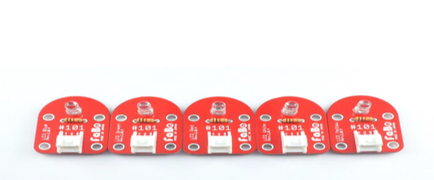
\includegraphics[width=6.473cm,height=3.66cm]{text05-img/text05-img015.png}
\captionof{figure}[LED]{LED}
 &
 回路記号 &

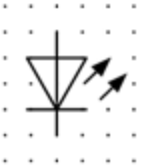
\includegraphics[width=3.985cm,height=4.593cm]{text05-img/text05-img042.png}
\captionof{figure}[LED]{LED}
\\\hline
\end{supertabular}
\end{flushleft}

\bigskip

\clearpage\subsubsection[\ 振動子]{\rmfamily \ 振動子}
\label{bkm:RefHeadingToc25513508239293}
\bigskip

\begin{flushleft}
\tablefirsthead{}
\tablehead{}
\tabletail{}
\tablelasttail{}
\begin{supertabular}{|m{4.2450004cm}|m{6.6260004cm}|}
\hline
 名称 &
\arraybslash 振動子(しんどうし)\\\hline
 接続箇所 &
\arraybslash デジタルコネクタ (3pin)\\\hline
 機能概要 &
\arraybslash 振動モーターでふるえる\\\hline
\end{supertabular}
\end{flushleft}

\bigskip

\begin{flushleft}
\tablefirsthead{}
\tablehead{}
\tabletail{}
\tablelasttail{}
\begin{supertabular}{|m{3.769cm}|m{12.844cm}|}
\hline
 サンプルコードの場所 &
\arraybslash ome/05/digout.hsp\\\hline
 raspiへの入力 &
\arraybslash なし\\\hline
 raspiへの入力方法 &
\arraybslash なし\\\hline
 raspiからの出力 &
\arraybslash
値が1のときふるえ、値が0のとき動かない\\\hline
 raspiからの出力方法 &
\arraybslash \ gpio GPIOの番号, パラメータ\\\hline
\end{supertabular}
\end{flushleft}

\bigskip


\bigskip

\begin{flushleft}
\tablefirsthead{}
\tablehead{}
\tabletail{}
\tablelasttail{}
\begin{supertabular}{|m{3.769cm}|m{12.844cm}|}
\hline
 使い道 &
\arraybslash
先に何かを付けて回転させる。せんぷうきなど。\\\hline
 注意事項 &
\arraybslash
振動している部分に触って怪我をしたり、壊したりしないように注意\\\hline
 補足 &
~
\\\hline
\end{supertabular}
\end{flushleft}

\bigskip

\begin{flushleft}
\tablefirsthead{}
\tablehead{}
\tabletail{}
\tablelasttail{}
\begin{supertabular}{|m{1.0699999cm}|m{6.4680004cm}|m{1.7049999cm}|m{6.9700003cm}|}
\hline
 外観 &
~


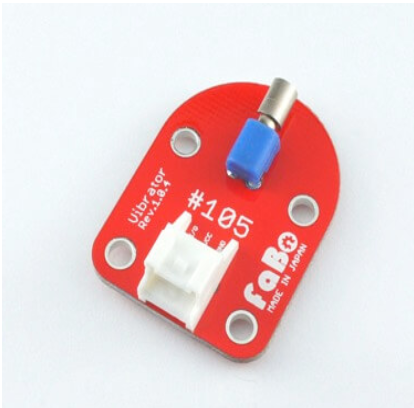
\includegraphics[width=6.473cm,height=6.378cm]{text05-img/text05-img016.png}
\captionof{figure}[振動子]{振動子}
 &
 回路記号 &

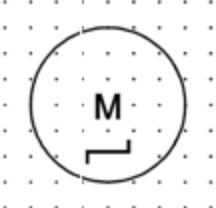
\includegraphics[width=6.387cm,height=6.149cm]{text05-img/text05-img043.png}
\captionof{figure}[振動子]{振動子}
\\\hline
\end{supertabular}
\end{flushleft}

\bigskip

\clearpage\subsection[デジタル入力そうち]{\rmfamily
デジタル入力そうち}
\subsubsection[ボタン]{\rmfamily ボタン}
\label{bkm:RefHeadingToc25515508239293}\begin{flushleft}
\tablefirsthead{}
\tablehead{}
\tabletail{}
\tablelasttail{}
\begin{supertabular}{|m{4.2450004cm}|m{6.6260004cm}|}
\hline
 名称 &
\arraybslash ボタン(ぼたん)\\\hline
 接続箇所 &
\arraybslash デジタルコネクタ (3pin)\\\hline
 機能概要 &
\arraybslash
ボタンが押されているか、押されていないかを調べる\\\hline
\end{supertabular}
\end{flushleft}

\bigskip

\begin{flushleft}
\tablefirsthead{}
\tablehead{}
\tabletail{}
\tablelasttail{}
\begin{supertabular}{|m{3.769cm}|m{12.844cm}|}
\hline
 サンプルコードの場所 &
\arraybslash ome/05/digin.hsp\\\hline
 raspiへの入力 &
\arraybslash
ボタンが押されていると0、押されていないと1の値になる。\\\hline
 raspiへの入力方法 &
\arraybslash val = gpioin(GPIO番号)\\\hline
 raspiからの出力 &
\arraybslash なし\\\hline
 raspiからの出力方法 &
\arraybslash なし\\\hline
\end{supertabular}
\end{flushleft}

\bigskip


\bigskip

\begin{flushleft}
\tablefirsthead{}
\tablehead{}
\tabletail{}
\tablelasttail{}
\begin{supertabular}{|m{3.769cm}|m{12.844cm}|}
\hline
 使い道 &
\arraybslash
ゲームのコントローラーのボタン\\\hline
 注意事項 &
\arraybslash
強く押して壊さないように注意\\\hline
 補足 &
\arraybslash
ボタンを押すことによって、中に入っている金属が繋がり電気が流れます。\\\hline
\end{supertabular}
\end{flushleft}

\bigskip

\begin{flushleft}
\tablefirsthead{}
\tablehead{}
\tabletail{}
\tablelasttail{}
\begin{supertabular}{|m{1.0699999cm}|m{6.4680004cm}|m{1.7049999cm}|m{6.9700003cm}|}
\hline
 外観 &
~


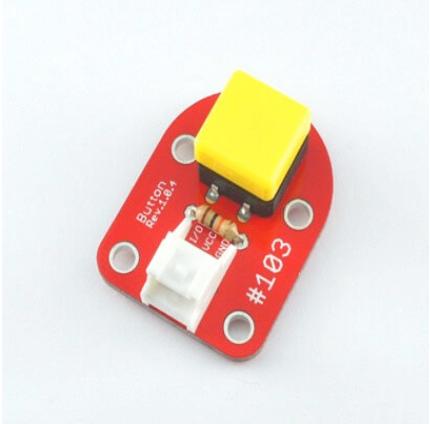
\includegraphics[width=6.473cm,height=6.382cm]{text05-img/text05-img005.png}
\captionof{figure}[ボタン]{ボタン}
 &
 回路記号 &

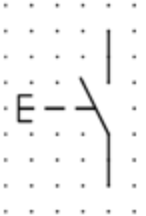
\includegraphics[width=4.463cm,height=6.602cm]{text05-img/text05-img044.png}
\captionof{figure}[ボタン]{ボタン}
\\\hline
\end{supertabular}
\end{flushleft}

\bigskip


\bigskip

\clearpage\subsubsection[\ \ 傾斜センサー]{\rmfamily
\ \ 傾斜センサー}
\label{bkm:RefHeadingToc25517508239293}\begin{flushleft}
\tablefirsthead{}
\tablehead{}
\tabletail{}
\tablelasttail{}
\begin{supertabular}{|m{4.2450004cm}|m{6.6670003cm}|}
\hline
 名称 &
\arraybslash
傾斜センサー(けいしゃせんさー)\\\hline
 接続箇所 &
\arraybslash デジタルコネクタ (3pin)\\\hline
 機能概要 &
\arraybslash
中のボールの転がりで、傾きを検知する\\\hline
\end{supertabular}
\end{flushleft}

\bigskip

\begin{flushleft}
\tablefirsthead{}
\tablehead{}
\tabletail{}
\tablelasttail{}
\begin{supertabular}{|m{3.769cm}|m{12.844cm}|}
\hline
 サンプルコードの場所 &
\arraybslash ome/05/digin.hsp\\\hline
 raspiへの入力 &
\arraybslash
センサーが傾くと1、傾いていないと値の値を入力します\\\hline
 raspiへの入力方法 &
\arraybslash val = gpioin(GPIO番号)\\\hline
 raspiからの出力 &
\arraybslash なし\\\hline
 raspiからの出力方法 &
\arraybslash なし\\\hline
\end{supertabular}
\end{flushleft}

\bigskip

\begin{flushleft}
\tablefirsthead{}
\tablehead{}
\tabletail{}
\tablelasttail{}
\begin{supertabular}{|m{3.769cm}|m{12.844cm}|}
\hline
 使い道 &
\arraybslash ストーブの安全装置\\\hline
 注意事項 &
\arraybslash なし\\\hline
 補足 &
{\centering
黒い箱のなかにボールが入っていて、ボールが転がり端子に触れるとONになります。傾いていないときはOFFになります。\par}

\captionof{figure}[傾斜センサーの内部]{
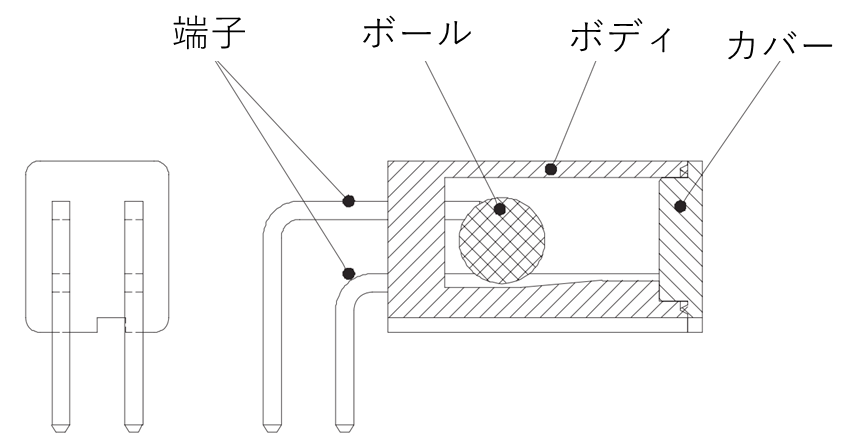
\includegraphics[width=12.85cm,height=6.595cm]{text05-img/text05-img045.png} \newline
傾斜センサーの内部}
\\\hline
\end{supertabular}
\end{flushleft}

\bigskip

\begin{flushleft}
\tablefirsthead{}
\tablehead{}
\tabletail{}
\tablelasttail{}
\begin{supertabular}{|m{1.0699999cm}|m{6.4680004cm}|m{1.7049999cm}|m{6.9700003cm}|}
\hline
\centering 外観 &
\centering \captionof{figure}[傾斜センサー]{
\includegraphics[width=5.773cm,height=6.789cm]{text05-img/text05-img017.png} \newline
傾斜センサー}
 &
\centering 回路記号 &
\centering\arraybslash \captionof{figure}[傾斜センサーの回路図]{
\includegraphics[width=6.061cm,height=4.202cm]{text05-img/text05-img046.png} \newline
傾斜センサーの回路図}
\\\hline
\end{supertabular}
\end{flushleft}

\bigskip

\clearpage\subsubsection[\ スイッチ]{\rmfamily \ スイッチ}
\label{bkm:RefHeadingToc25519508239293}
\bigskip

\begin{flushleft}
\tablefirsthead{}
\tablehead{}
\tabletail{}
\tablelasttail{}
\begin{supertabular}{|m{4.2450004cm}|m{6.6260004cm}|}
\hline
\centering 名称 &
\centering\arraybslash スイッチ(すいっち)\\\hline
\centering 接続箇所 &
\centering\arraybslash デジタルコネクタ (3pin)\\\hline
\centering 機能概要 &
\centering\arraybslash ONとOFFを切りかえる\\\hline
\end{supertabular}
\end{flushleft}

\bigskip

\begin{flushleft}
\tablefirsthead{}
\tablehead{}
\tabletail{}
\tablelasttail{}
\begin{supertabular}{|m{3.769cm}|m{12.844cm}|}
\hline
\centering サンプルコードの場所 &
\centering\arraybslash ome/05/digin.hsp\\\hline
\centering raspiへの入力 &
\centering\arraybslash
右にスライドさせると1、左にスライドさせると0を入力する\\\hline
\centering raspiへの入力方法 &
\centering\arraybslash val = gpioin(GPIO番号)\\\hline
\centering raspiからの出力 &
\centering\arraybslash なし\\\hline
\centering raspiからの出力方法 &
\centering\arraybslash なし\\\hline
\end{supertabular}
\end{flushleft}

\bigskip

\begin{flushleft}
\tablefirsthead{}
\tablehead{}
\tabletail{}
\tablelasttail{}
\begin{supertabular}{|m{3.769cm}|m{12.844cm}|}
\hline
\centering 使い道 &
\centering\arraybslash 照明のスイッチ\\\hline
\centering 注意事項 &
\centering\arraybslash なし\\\hline
\centering 補足 &
\centering\arraybslash
ボタンと違い、人の手を使わなくとも値を保持しておくことができます。\\\hline
\end{supertabular}
\end{flushleft}

\bigskip

\begin{flushleft}
\tablefirsthead{}
\tablehead{}
\tabletail{}
\tablelasttail{}
\begin{supertabular}{|m{1.0699999cm}|m{6.4680004cm}|m{1.7049999cm}|m{6.9700003cm}|}
\hline
\centering 外観 &
\includegraphics[width=5.682cm,height=5.998cm]{text05-img/text05-img018.jpg}\captionof{figure}[スイッチ]{スイッチ}

~
 &
\centering 回路記号 &
\centering\arraybslash \captionof{figure}[スイッチの回路図]{
\includegraphics[width=6.061cm,height=4.202cm]{text05-img/text05-img046.png} \newline
スイッチの回路図}
\\\hline
\end{supertabular}
\end{flushleft}
\subsubsection[]{\rmfamily }
\clearpage\subsubsection[\ リミットスイッチ]{\rmfamily
\ リミットスイッチ}
\label{bkm:RefHeadingToc25709508239293}
\bigskip

\begin{flushleft}
\tablefirsthead{}
\tablehead{}
\tabletail{}
\tablelasttail{}
\begin{supertabular}{|m{4.2450004cm}|m{6.663cm}|}
\hline
\centering 名称 &
\centering\arraybslash
リミットスイッチ(りみっとすいっち)\\\hline
\centering 接続箇所 &
\centering\arraybslash デジタルコネクタ (3pin)\\\hline
\centering 機能概要 &
\centering\arraybslash ONとOFFを検知する\\\hline
\end{supertabular}
\end{flushleft}

\bigskip

\begin{flushleft}
\tablefirsthead{}
\tablehead{}
\tabletail{}
\tablelasttail{}
\begin{supertabular}{|m{3.769cm}|m{12.844cm}|}
\hline
\centering サンプルコードの場所 &
\centering\arraybslash ome/05/digin.hsp\\\hline
\centering raspiへの入力 &
\centering\arraybslash
スイッチが押されていると1、押されていないと0の値になる\\\hline
\centering raspiへの入力方法 &
\centering\arraybslash val = gpioin(GPIO番号)\\\hline
\centering raspiからの出力 &
\centering\arraybslash なし\\\hline
\centering raspiからの出力方法 &
\centering\arraybslash なし\\\hline
\end{supertabular}
\end{flushleft}

\bigskip

\begin{flushleft}
\tablefirsthead{}
\tablehead{}
\tabletail{}
\tablelasttail{}
\begin{supertabular}{|m{3.769cm}|m{12.844cm}|}
\hline
\centering 使い道 &
\centering\arraybslash
ロボットが壁に触れたかどうかわかる。\newline
蓋がしまっているかどうかわかる。\\\hline
\centering 注意事項 &
\centering\arraybslash なし\\\hline
\centering 補足 &
\centering\arraybslash なし\\\hline
\end{supertabular}
\end{flushleft}

\bigskip

\begin{flushleft}
\tablefirsthead{}
\tablehead{}
\tabletail{}
\tablelasttail{}
\begin{supertabular}{|m{1.0699999cm}|m{6.4680004cm}|m{1.7049999cm}|m{6.9700003cm}|}
\hline
\centering 外観 &
\includegraphics[width=4.89cm,height=6.113cm]{text05-img/text05-img019.jpg}\captionof{figure}[リミットスイッチ]{リミットスイッチ}
 &
\centering 回路記号 &
\centering\arraybslash
\captionof{figure}[リミットスイッチの回路図]{
\includegraphics[width=6.976cm,height=2.685cm]{text05-img/text05-img047.png} \newline
リミットスイッチの回路図}
\\\hline
\end{supertabular}
\end{flushleft}
\subsection[]{\rmfamily }
\clearpage\subsection[アナログ入力そうち]{\rmfamily
アナログ入力そうち}
\label{bkm:RefHeadingToc4569508239293}\subsubsection[\ 感圧センサー]{\rmfamily
\ 感圧センサー}
\label{bkm:RefHeadingToc25711508239293}\begin{flushleft}
\tablefirsthead{}
\tablehead{}
\tabletail{}
\tablelasttail{}
\begin{supertabular}{|m{4.2450004cm}|m{6.663cm}|}
\hline
\centering 名称 &
\centering\arraybslash
感圧センサー(かんあつせんさー)\\\hline
\centering 接続箇所 &
\centering\arraybslash アナログコネクタ (3pin)\\\hline
\centering 機能概要 &
\centering\arraybslash 圧力を測定する\\\hline
\end{supertabular}
\end{flushleft}

\bigskip

\begin{flushleft}
\tablefirsthead{}
\tablehead{}
\tabletail{}
\tablelasttail{}
\begin{supertabular}{|m{3.769cm}|m{12.844cm}|}
\hline
\centering サンプルコードの場所 &
\centering\arraybslash ome/05/anain.hsp\\\hline
\centering raspiへの入力 &
\centering\arraybslash
0〜1023の値で圧力を測定します。圧力がかかるほど値が小さくなります。\\\hline
\centering raspiへの入力方法 &
\centering\arraybslash val = spiget(ピン番号,
チャンネル番号)\\\hline
\centering raspiからの出力 &
\centering\arraybslash なし\\\hline
\centering raspiからの出力方法 &
\centering\arraybslash なし\\\hline
\end{supertabular}
\end{flushleft}

\bigskip

\begin{flushleft}
\tablefirsthead{}
\tablehead{}
\tabletail{}
\tablelasttail{}
\begin{supertabular}{|m{3.769cm}|m{12.844cm}|}
\hline
\centering 使い道 &
\centering\arraybslash
圧力を調べる、重さをはかる\\\hline
\centering 注意事項 &
\centering\arraybslash
圧力を感知する部分が壊れやすいです。\\\hline
\centering 補足 &
\centering\arraybslash なし\\\hline
\end{supertabular}
\end{flushleft}

\bigskip

\begin{flushleft}
\tablefirsthead{}
\tablehead{}
\tabletail{}
\tablelasttail{}
\begin{supertabular}{|m{1.0699999cm}|m{6.4680004cm}|m{1.7049999cm}|m{6.9700003cm}|}
\hline
\centering 外観 &
\includegraphics[width=5.194cm,height=5.871cm]{text05-img/text05-img020.jpg}\captionof{figure}[感圧センサー]{感圧センサー}
 &
\centering 回路記号 &
\centering\arraybslash \captionof{figure}[感圧センサーの回路図]{
\includegraphics[width=4.2cm,height=2.997cm]{text05-img/text05-img048.png} \newline
感圧センサーの回路図}
\\\hline
\end{supertabular}
\end{flushleft}
\subsubsection*{\rmfamily }
\clearpage\subsubsection{ボリューム}
\label{bkm:RefHeadingToc25713508239293}\begin{flushleft}
\tablefirsthead{}
\tablehead{}
\tabletail{}
\tablelasttail{}
\begin{supertabular}{|m{4.2450004cm}|m{6.6260004cm}|}
\hline
\centering 名称 &
\centering\arraybslash ボリューム(ぼりゅーむ)\\\hline
\centering 接続箇所 &
\centering\arraybslash アナログコネクタ (3pin)\\\hline
\centering 機能概要 &
\centering\arraybslash つまみの回転量を出力\\\hline
\end{supertabular}
\end{flushleft}

\bigskip

\begin{flushleft}
\tablefirsthead{}
\tablehead{}
\tabletail{}
\tablelasttail{}
\begin{supertabular}{|m{3.769cm}|m{12.844cm}|}
\hline
\centering サンプルコードの場所 &
\centering\arraybslash ome/05/anain.hsp\\\hline
\centering raspiへの入力 &
\centering\arraybslash つまみの回転量 0から1023の値\\\hline
\centering raspiへの入力方法 &
\centering\arraybslash val = spiget(ピン番号,
チャンネル番号)\\\hline
\centering raspiからの出力 &
\centering\arraybslash なし\\\hline
\centering raspiからの出力方法 &
\centering\arraybslash なし\\\hline
\end{supertabular}
\end{flushleft}

\bigskip

\begin{flushleft}
\tablefirsthead{}
\tablehead{}
\tabletail{}
\tablelasttail{}
\begin{supertabular}{|m{3.769cm}|m{12.844cm}|}
\hline
\centering 使い道 &
\centering\arraybslash 音量調整, LEDの明るさ調整,
ゲームのコントローラとして\\\hline
\centering 注意事項 &
\centering\arraybslash
力を入れすぎて壊れないよう注意\\\hline
\centering 補足 &
{\centering
先端のつまみをつまんで回転させると抵抗値が変化しraspberry
piに入力される電圧が変化します。今回使うボリュームは左に回しきったときは変化が小さく、右に回すほど変化が大きくなります(指数関数的)。この設定をAカーブと呼びます
(図\ref{seq:refIllustration15})。これはボリュームがしばしば音量調節に利用され、人間の耳の感度は対数関数的(小さい音ほど敏感で大きい音に関しては鈍感)であることからこのように設定されています。もちろん、ボリュームは音量調節以外にも使用されるため、用途に応じて特性が線形(傾きが一定)なBカーブや対数関数的(傾きが小さくなっていく)なCカーブなどが存在します。\par}

\centering
\captionof{figure}[ボリュームの特性]{
\includegraphics[width=5.537cm,height=3.493cm]{text05-img/text05-img049.jpg} \newline
ボリュームの特性}
\label{seq:refIllustration15}
\centering
\captionof{figure}[ボリュームの仕組み]{
\includegraphics[width=11.668cm,height=4.471cm]{text05-img/text05-img050.png} \newline
ボリュームの仕組み}
\label{seq:refIllustration16}
{\centering
ボリュームには端子が3つ付いており、図\ref{seq:refIllustration16}のように1つに+電源を、1つに-電源をつなげ、もう1つを出力として使用します。+電源から-電源までに帯状の抵抗器が接続されており、その間に出力の端子が接続されています。シャフトを回すことで、出力端子の位置が変化し、結果プラス電源端子{}-出力端子間と\par}

\centering\arraybslash
出力端子-マイナス電源端子間の抵抗値が変化することになります。\\\hline
\end{supertabular}
\end{flushleft}

\bigskip

\begin{flushleft}
\tablefirsthead{}
\tablehead{}
\tabletail{}
\tablelasttail{}
\begin{supertabular}{|m{1.0699999cm}|m{6.4680004cm}|m{1.7049999cm}|m{6.9700003cm}|}
\hline
\centering 外観 &
\centering \captionof{figure}[: ]{ \includegraphics[width=6.858cm,height=5.131cm]{text05-img/text05-img021.jpg} \newline
: }
 &
\centering 回路記号 &
\centering\arraybslash \captionof{figure}[: ]{
\includegraphics[width=1.711cm,height=1.198cm]{text05-img/text05-img051.png} \newline
: }
\\\hline
\end{supertabular}
\end{flushleft}
\clearpage\subsubsection[\ 距離センサー]{\rmfamily
\ 距離センサー}
\label{bkm:RefHeadingToc5917367650265}\begin{flushleft}
\tablefirsthead{}
\tablehead{}
\tabletail{}
\tablelasttail{}
\begin{supertabular}{|m{4.2450004cm}|m{6.6260004cm}|}
\hline
\centering 名称 &
\centering\arraybslash
距離センサー(きょりせんさー)\\\hline
\centering 接続箇所 &
\centering\arraybslash アナログコネクタ (3pin)\\\hline
\centering 機能概要 &
\centering\arraybslash
センサーから障害物までの距離を計測\\\hline
\end{supertabular}
\end{flushleft}

\bigskip

\begin{flushleft}
\tablefirsthead{}
\tablehead{}
\tabletail{}
\tablelasttail{}
\begin{supertabular}{|m{3.769cm}|m{12.844cm}|}
\hline
 サンプルコードの場所 &
\arraybslash ome/05/anain.hsp\\\hline
 raspiへの入力 &
\arraybslash
距離をあらわす0から1023の値。測定可能な距離は10cmから80cm。\\\hline
 raspiへの入力方法 &
\arraybslash val = spiget(ピン番号,
チャンネル番号)\\\hline
 raspiからの出力 &
\arraybslash なし\\\hline
 raspiからの出力方法 &
\arraybslash なし\\\hline
\end{supertabular}
\end{flushleft}

\bigskip

\begin{flushleft}
\tablefirsthead{}
\tablehead{}
\tabletail{}
\tablelasttail{}
\begin{supertabular}{|m{3.769cm}|m{12.844cm}|}
\hline
 使い道 &
\arraybslash
距離計測、障害物センサーとして。\\\hline
 注意事項 &
\arraybslash
レンズを覗き込むと目に影響を及ぼすことがあるため覗き込まないこと。\\\hline
 補足 &
{
入力の単位はセンチメートルではないため、変換が必要です。出力は0から1023で出力されるので、これを数式1
で変換する必要があります。数式\ref{seq:ref0}の
$x$
にセンサーからのデータを代入することでセンチメートルへの変換が可能です。\par}

\begin{minipage}{3.784cm}
{\upshape  $-\frac 1{36}\times \frac{5000}{1023}x+\frac{845} 9$ 数式
{\refstepcounter{qwertyc}\theqwertyc\label{seq:ref0}}}\end{minipage}
三角測量の原理により、ある三角形があったとき一辺の長さとそれに対する角の角度がわかれば三角形が決定します(余弦定理)。距離センサーは光源と受光器で成っています。受光器は光源が反射してきた光の位置を計測することが出来ます。光源と受光器は固定されているので、その間の距離と対する角の角度がわかり、これと三角関数を使うと距離が求まります\\\hline
\end{supertabular}
\end{flushleft}

\bigskip

\begin{flushleft}
\tablefirsthead{}
\tablehead{}
\tabletail{}
\tablelasttail{}
\begin{supertabular}{|m{1.0699999cm}|m{6.4680004cm}|m{1.7049999cm}|m{6.9700003cm}|}
\hline
 外観 &
 \captionof{figure}[: ]{ \includegraphics[width=5.944cm,height=4.42cm]{text05-img/text05-img022.jpg} \newline
: }
 &
 回路記号 &
\arraybslash 回路記号はありません。\\\hline
\end{supertabular}
\end{flushleft}
\subsubsection[]{\rmfamily }
\clearpage\subsubsection[\ 照度センサー]{\rmfamily
\ 照度センサー}
\label{bkm:RefHeadingToc25715508239293}\begin{flushleft}
\tablefirsthead{}
\tablehead{}
\tabletail{}
\tablelasttail{}
\begin{supertabular}{|m{4.2450004cm}|m{6.6260004cm}|}
\hline
 名称 &
\arraybslash
照度センサー(しょうどせんさー)\\\hline
 接続箇所 &
\arraybslash アナログコネクタ (3pin)\\\hline
 機能概要 &
\arraybslash 周辺の明るさの測定\\\hline
\end{supertabular}
\end{flushleft}

\bigskip

\begin{flushleft}
\tablefirsthead{}
\tablehead{}
\tabletail{}
\tablelasttail{}
\begin{supertabular}{|m{3.769cm}|m{12.844cm}|}
\hline
 サンプルコードの場所 &
\arraybslash ome/05/anain.hsp\\\hline
 raspiへの入力 &
\arraybslash
明るさを表す0から1023の値。明るいと値が減り、暗いと値が増える。\\\hline
 raspiへの入力方法 &
\arraybslash val = spiget(ピン番号,
チャンネル番号)\\\hline
 raspiからの出力 &
\arraybslash なし\\\hline
 raspiからの出力方法 &
\arraybslash なし\\\hline
\end{supertabular}
\end{flushleft}

\bigskip

\begin{flushleft}
\tablefirsthead{}
\tablehead{}
\tabletail{}
\tablelasttail{}
\begin{supertabular}{|m{3.769cm}|m{12.844cm}|}
\hline
 使い道 &
\arraybslash
照度計測、カメラの露出調節機能に。\\\hline
 注意事項 &
\arraybslash
材料の硫化カドミウム(CdS)は人体に有害なため、割れたセンサーを素手で触らないこと。\\\hline
 補足 &
\arraybslash なし\\\hline
\end{supertabular}
\end{flushleft}

\bigskip

\begin{flushleft}
\tablefirsthead{}
\tablehead{}
\tabletail{}
\tablelasttail{}
\begin{supertabular}{|m{1.0699999cm}|m{6.4680004cm}|m{1.7049999cm}|m{6.9700003cm}|}
\hline
 外観 &
 \includegraphics[width=5.946cm,height=6.008cm]{text05-img/text05-img023.png}\captionof{figure}[: ]{\newline
: }
 &
 回路記号 &
\arraybslash 
\includegraphics[width=6.976cm,height=3.715cm]{text05-img/text05-img052.png}\captionof{figure}[: ]{\newline
: }
\\\hline
\end{supertabular}
\end{flushleft}

\bigskip

\clearpage\subsection[ゆうきELディスプレイ]{\rmfamily
ゆうきELディスプレイ}
\label{bkm:RefHeadingToc25717508239293}
\bigskip

\begin{flushleft}
\tablefirsthead{}
\tablehead{}
\tabletail{}
\tablelasttail{}
\begin{supertabular}{|m{4.2450004cm}|m{10.569cm}|}
\hline
 名称 &
\arraybslash
有機ELディスプレイ(ゆうきいーえるでぃすぷれい)\\\hline
 接続箇所 &
\arraybslash I2C (4pin)\\\hline
 機能概要 &
\arraybslash 文字の表示\\\hline
\end{supertabular}
\end{flushleft}

\bigskip

\begin{flushleft}
\tablefirsthead{}
\tablehead{}
\tabletail{}
\tablelasttail{}
\begin{supertabular}{|m{3.769cm}|m{12.844cm}|}
\hline
 サンプルコードの場所 &
\arraybslash ome/05/oled.hsp\\\hline
 raspiへの入力 &
\arraybslash なし\\\hline
 raspiへの入力方法 &
\arraybslash なし\\\hline
 raspiからの出力 &
\arraybslash
プログラムで決めた文字や記号を表示する\\\hline
 raspiからの出力方法 &
\arraybslash oled ``表示させたい文字''\\\hline
\end{supertabular}
\end{flushleft}

\bigskip

\begin{flushleft}
\tablefirsthead{}
\tablehead{}
\tabletail{}
\tablelasttail{}
\begin{supertabular}{|m{3.769cm}|m{12.844cm}|}
\hline
 使い道 &
\arraybslash テレビ\\\hline
 注意事項 &
\arraybslash
日本語表示させることはできないので注意\\\hline
 補足 &
\arraybslash なし\\\hline
\end{supertabular}
\end{flushleft}

\bigskip

\begin{flushleft}
\tablefirsthead{}
\tablehead{}
\tabletail{}
\tablelasttail{}
\begin{supertabular}{|m{1.0699999cm}|m{6.4680004cm}|m{1.7049999cm}|m{6.9700003cm}|}
\hline
 外観 &
 \includegraphics[width=5.946cm,height=5.786cm]{text05-img/text05-img024.png}\captionof{figure}[: ]{\newline
: }
 &
 回路記号 &
\arraybslash 回路記号はありません。\\\hline
\end{supertabular}
\end{flushleft}

\bigskip

\clearpage\section[参考文献]{\rmfamily\color{black} 参考文献}
\begin{itemize}
\item \textcolor{black}{樋口龍雄, 川又政征.
MATLAB対応ディジタル信号処理. 森北出版.
2015.}
\end{itemize}
\begin{itemize}
\item \textcolor{black}{日本産業標準調査会.
電気用図記号. 2011. (規格番号 JISC0617)}
\item Fabo, Inc\newline
\url{http://www.fabo.io/}
\item ナルガッキ.
ボリューム、トーンに適したポットのカーブの特徴と違い.
(図\ref{seq:refIllustration15})\newline
\url{https://naru-gakki.com/pot-curve/}\ \ \ \ \ \ \ \ \ \ \ \ \ \ \ \ \ \ \ \ \ \ \ \ \ \ \ \ \ \ \ \ \ \ \ \ \ \ \ \ \ \ \ \ \ \ \ \ \ \ \ \ \ \ \ \ \ \ \ \ \ \ \ \ \ \ \ \ \ \ \ \ \ \ 
\end{itemize}
\end{document}
